\documentclass[]{article}
\usepackage[left=3cm,right=3cm,top=1.5cm,bottom=2cm,includeheadfoot]{geometry} 
\usepackage{babel}
\usepackage{hyperref}
\usepackage{mwe}
\usepackage[markcase=noupper]{scrlayer-scrpage}
\usepackage{amsmath}
\usepackage{amssymb}
\usepackage{multirow}
\usepackage{subcaption}
\usepackage{rotating}

\usepackage{setspace}
\usepackage{graphicx}
\usepackage{forest}
\usepackage{tikz-qtree}

% bibliography natbib
\usepackage[numbers]{natbib}
\bibliographystyle{abbrvnat}
%\setcitestyle{authoryear, open={((},close={))}
\renewcommand{\cite}{\citep}
\newcommand{\titletitle}{Finding Gene Expression Patterns and their Link to Connectivities in Mouse Brains by Exploiting Interaction Networks }


% configure headline

\ihead{Tilman Hinnerichs}
\ohead{Gene Expression Patterns and their Link to Connectivities in Mouse Brains}
%\ohead{Linking Connectivities and Gene Expression Patterns in the Mouse Brain}
\cfoot*{\pagemark}
%opening
\title{\titletitle}
\author{Tilman Hinnerichs}
\date{}
\pagestyle{headings}

% Build subsubsubsection
\usepackage{titlesec}
\usepackage{todonotes}

%Definitions
\newtheorem{mydef}{Definition}
\newtheorem{example}{Example}
\newtheorem{lemma}{Lemma}
\newtheorem{theorem}{Theorem}
\newtheorem{corollary}{Corollary}
\newtheorem{proposition}{Proposition}

\newcommand{\name}{Treasure}
\newcommand{\Github}{https://github.com/neural-data-science-lab/Treasure-Gene-expression-regions}

\newcommand{\HRule}[1]{\rule{\linewidth}{#1}}
\setcounter{tocdepth}{5}
\setcounter{secnumdepth}{5}

%-------------------------------------------------------------------------------
% TITLE PAGE
%-------------------------------------------------------------------------------

\begin{document}
	
\emergencystretch 3em
	
\onehalfspacing
	
\pagenumbering{gobble}
\thispagestyle{empty}
	
\title{ \normalsize \textsc{Diploma thesis}
	\\ [2.0cm]
	\HRule{0.5pt} \\
	\LARGE \textbf{\uppercase{Finding Gene Expression Patterns and their Link to Connectivities in Mouse Brains by Exploiting Interaction Networks}
		\HRule{1pt} \\ [0.5cm]
		\normalsize \vspace*{5\baselineskip}}
	
	{\normalsize
	Tilman Hinnerichs \\
	Matrikelnummer: 4643427 \\ 
	Technische Universität Dresden\vspace{1cm}\\
	External supervisor: Dr. Nico Scherf\\
	Max Planck Institute for Human Cognitive and Brain Sciences\\}
	\author{
		}
	
	\begin{flushleft}
		\normalsize
		\vspace{2cm}
		Supervising professor:\\
		Prof. Dr. rer. med. Ingo Röder\\
		\vspace{0.25cm}
		Advisory professor:\\
		Prof. Dr. Michael Schröder\\
		\vspace{1cm}
		Submitted on August 10, 2022
	\end{flushleft}}
\maketitle

%\section*{Statement of authorship}
%I hereby certify that I have authored this document entitled ``\titletitle'' independently and without undue assistance from third parties. No
%other than the resources and references indicated in this document have been used. I have
%marked both literal and accordingly adopted quotations as such. There were no additional
%persons involved in the intellectual preparation of the present document. I am aware that
%violations of this declaration may lead to subsequent withdrawal of the academic degree.\\
%
%Dresden, 10.08.2022\\
%
%\vspace{0.25cm}
%Tilman Hinnerichs\\
%
%\vspace{0.15cm}
%\hspace{0.6cm}\includegraphics[width=0.25\textwidth]{../../../../Wichtig/digital_sign.png}
%
%\newpage
\begin{abstract}
	Improvements in finding gene expression patterns and their spatial distribution among different tissues help to identify spatial organization and inter-structure relations. Moreover, they help to understand disturbances in embryogenesis and malignant tissue evolution. Multiple studies showed the correlation of gene expression patterns and cognition, behavior and their pathology. However, these approaches are primarily concerned with inter-structure relations but neglect the gravity of inter-gene networks. We thus try to exploit protein-protein interaction networks for finding gene expression patterns and their influence on structural, functional and effective brain connectivity. Violation of such brain wiring is linked to brain disorders and diseases, while spatial gene expression is correlated with all three connectivity types. \\
	Recent advances in sequencing methodology allow for measurement of expression levels for thousands of genes in the respective tissues. We apply graph convolutional neural networks (GCNs) for the three tasks of (1) predicting gene expression from molecular and phenotypical features, (2) learning gene expression patterns over unsupervised dimensionality reduction and (3) predict inter-structure connectivities based on these gene expression patterns. We introduce two metrics for the unsupervised learning task and show that GCNs consistently improve over the non-GCN baseline methods for dimensionality reduction and connectivity prediction. \\
	We find associations of \textit{gene importance} in the networks and neurotransmitter related proteins and thus conclude the significance of gene-gene relations for neural activity patterns. This study may hence leverage advances in understanding of pathogenesis for brain disorders.
\end{abstract}

\newpage

\tableofcontents

\newpage


%\subsection*{To be sorted somewhere}
%\begin{itemize}
%	\item Variability and different interpretations of different graph convolutional neural filters \cite{GCNConv, GENConv2020, feng2022kergnns} etc.
%	
%	
%	\item DeepGOPlus for feature generation \cite{DeepGoPlus}
%	\item discussion of different PPI network databases \cite{STRINGv10}
%	\item discussion of potential databases associating gene expression data with their spatial distribution \cite{hawrylycz_digital_2011}
%	\item discussion of best neural learning/graph convolutional methods \cite{Pytorch, PytorchGeometric}
%	\item how to handle highly imbalanced data, metrics, preprocessing, sampling, modification of loss function \cite{Jeni2013} and optimization over them (with Adam\cite{Adam2014})
%	\item maybe introduction of PhenomeNET for MP/GO for more sophisticated protein representation \cite{PhenomeNET2011, GOoriginal2000, GOrecent2020, MP2009} and derive features from DL2vec \cite{DL2vec2020, Word2vec2013}
%	\item evaluation of \glqq Using ontology embeddings for structural inductive bias in gene expression data analysis\grqq{}\cite{Trebacz2020}
%	\item take some ideas from \citet{Zitnik2017} with title \glqq Predicting multicellular function through multi-layer tissue networks\grqq{}. (OhmNet)
%	\item potentially group results based on InterPro\cite{Interpro2020} families eventually
%	
%	\item choice of model organism?!
%\end{itemize}
%
%
%\newpage

\thispagestyle{empty}
\listoffigures
\newpage
\listoftables
\newpage
\pagenumbering{arabic}

\section{Introduction}
\label{sec:introduction}
Gene expression analysis and their respective spatial patterns are essential for discovering the influence of biological processes within different tissues. Investigation of both pathological and non-pathological transcriptomic motifs may yield novel insights into inter- and intra-cellular pathways and their disturbance genesis. 
More specifically, cancerous tissues may be well defined by their corresponding abnormal expression fingerprint and thus lead to characterization of malignomas and their expected priors and temporal evolution. Similar analyses was applied in embryogenesis, but also adolescent and adult organisms, for disambiguation and further understanding of organ compartments.\\

One of the most complex and least understood organs across all entities in the animal kingdom is the \textit{brain}, combining both information processing and forwarding. Especially the human brain remains one of the most complicated and convoluted structures, but also among the most crucial for better understanding of cognition and behavior. 
The brain is a multi-level system in which high-level activities are determined by low-level, i.e. genetic mechanisms. Hence, decoding the linkage across multiple brain levels utilizing predictive and correlative investigation is one of the most important areas of brain research. Studies across multiple animal species demonstrate the correlation of brain wiring and spatial gene expression organization.\\

While malignant tissue and tumor genesis and evolution is among the most important questions for other tissues, other prevalent pathologies arise in the brain. Therefore, gene expression has been linked to a variety of brain related diseases in humans. More specifically, \citet{twine2011whole} show the correlation of spatial gene expression patterns and their aberrations to Alzheimer's disease. Moreover, other studies have shown circadian patterns of gene expression in human brain and the disruption of those in depressive disorders \cite{li2013circadian}. 

However, as aggregation of gene expression data for human brains remains difficult due to ethical reasons, researchers thus focus on various model organisms, also caused by their reduced complexity. Numerous publications aim to investigate the cognition of vertebrates such as \textit{Drosophila melanogaster} and nematodes such as \textit{Caenorhabditis elegans}, but also species within the same \textit{phylum} as humans like other mammals such as \textit{rodents} like \textit{Mus musculus} \cite{bohland2010clustering} and monkeys like \textit{Macaques} \cite{ValkShapingBrainStructure2020}. As non-\textit{Chordata} animals are less convoluted than mammals, a complete understanding, mapping and investigation may be feasible. On the other hand mammals are closer in behavior and structure to us humans, and thus may yield further understanding of our own organization. \\
One of the most examined model organisms is \textit{Mus musculus}, which is studied and surveyed extensively, and helped to yield numerous insights into our own biological and neurological systems. Moreover, various atlases describing the spatial distribution of mouse brains for gene expression data and cognition were published. We thus decided to analyze the gene expression values from the Allen Mouse Brain Atlas and combine them with various connectivity measures to better understand the underlying brain wiring within mice, to enhance comprehension of our own species. We therefore aim to first understand the sane brain and its circuits before tackling pathological data. Thus, we will only consider \textit{healthy} mouse brains and their respective organization.\\

Terms like \textit{brain wiring} may be stated in multiple ways. We thus follow the definitions of \citet{sporns2016networks} dividing brain connectivities into three sub-categories: (1) \textit{Axonal} or \textit{structural connectivity} links to physical or anatomical associations in form of neural elements and neurons, (2) \textit{functional connectivity} measuring anomalies from statistical independence between spatially remote and distributed neuronal units in their respective neural activity, and (3) \textit{effective connectivity} concerned with the causal effects and relations of brain compartments, i.e. actual collaboration and their dependencies. While we explore the range of related works in Section \ref{sec:relatedwork_conn}, we will motivate the underlying reasoning here. \citet{friston2002dysfunctional} states the so-called ``Disconnection Hypotheses'', and expresses the correlation of pathological cognitive behavior and abnormal alterations of connections. Multiple studies find such correlations across various species on one hand, and the correlation of all three connectivity types and spatial gene expression patterns. Further they may be a prior to the brain network's response to pathological perturbations \cite{fornito2015connectomics}. Determining that prior across all three connectivities is crucial for deciphering brain disorders and behavior. Advancements in bridging the gap from gene expression patterns may help doing so.\\

Such gene expression patterns may be articulated either in inter-structures dependencies, i.e. spatial organization of expressing genes, or in inter-gene relations, i.e. linkage of the transcriptome. Most related approaches focus on the first, which remains the final goal for this task, but neglect the inter-gene relations. These relations are non-trivial to describe, but crucial for further understanding of the associated biological processes. We hypothesize them facilitating further investigations and performance enhancement following the ``guilt by association'' principle \cite{Oliver2000, Gillis2012}.
Protein-protein interaction (PPI) graphs directly describe such links, but reveal information in cellular behavior and its functionality, too. Sub-structures and -graphs may e.g. characterize biological pathway information and model regulatory sub-networks or signaling paths. However, they only describe a two-entity database, but no inherent approach for incorporation to automated feature extraction methods. \\

Advancements in machine learning in form of graph convolutional neural networks (GCNs) may allow us to exploit such graph structures in order to exploit gene-gene relations. Generally, GCNs support the testing of different interpretations of the underlying graph by application of diversified graph convolutional neural filters, used for message passing. GCNs were first formulated in \citet{GCNConv} for supervised and semi-supervised learning, and allow for graph, node and edge representation and classification. Different types of formulations for message passing through the network were proposed such as Chebyshev \cite{ChebConv} and ARMA \cite{ArmaConv} filters, attention mechanisms \cite{GATConv} and random walk-based methods to further explore the node neighborhood \cite{APPNPConv, SAGEConv}. GCNs have two major limitations: (1) The issue of oversmoothing across node features caused by the message passing scheme, and (2) the restraint of hand-crafted combinatorial features of graphs for kernel filters. The limited ability to differentiate between neighboring node representations may be overcome by special feature propagation \cite{GENConv2020}, while subgraph-based filters \citet{feng2022kergnns} may improve expressivity, i.e. homorphism to the Weifeiler-Lehman algorithm \cite{leman1968reduction}. 
GCNs were successfully applied over PPI graphs for prediction of protein functions \cite{Zitnik2017}, drug-target interaction prediction \cite{hinnerichs2021dti} but also gene expression prediction in human tissue \cite{schulte2021integration, wang2021mogonet}.\\ 

Our study of the mouse brain transcriptome may be divided into two parts, describing three successive tasks, with varying assumptions, data and associated hypotheses. 
The first part is concerned with the prediction of gene expression data, whereas we try to predict based on the transcriptome within the second formulation. 
The prediction of gene expression patterns has a long history, which we describe in further detail in Section \ref{sec:relatedwork_geneexp}. Advancing model architectures exploiting different kinds of information may yield deeper insights into other down-stream and regulatory processes, and their corresponding pathology. In our first task, we follow the work of \citet{wang2021mogonet} and \citet{schulte2021integration}, applying graph convolutional neural networks for gene expression prediction, examining the influence of protein-protein interactions, but on spatial mouse brain data.\\

Additionally, we perform two separate learning tasks by representing each mouse brain compartment with its respective gene expression values, and determine the influence of GCNs on the model's expressivity. We do so by applying the same encoding model and therefore compare GCN and non-GCN-based models.
In the second task, we try to first derive brain compartments based on a unsupervised dimensionality reduction formulation. Doing so provides a native measure and intuition of feature and thus gene importance and further facilitates structure-specific down-stream prediction tasks, such as stroke prediction.
We do so by applying various embedding techniques such as PCA \cite{wold1987principal}, t-SNE \cite{van2008visualizing} and UMAP  \cite{mcinnes2018umap} to each brain structure representation. Uniform Manifold Approximation and Projection (UMAP) and its direct descendant Parametric UMAP \cite{sainburg2021parametric} are among the most recent and most successful, current dimensionality reduction techniques. Both are neural network-based approaches, and try to preserve local proximity within domain space in the embedding space. Due to their deep neural network character, they allow for a natural incorporation of the graph convolutional encoding model. 
Third, apply the same encoding model within a Siamese neural network directly trained for the task of connectivity prediction, over all three network types. Again, we hypothesize that while \textit{gene importance} for these were extensively studied for this purpose \cite{bohland2010clustering, ValkShapingBrainStructure2020, takata_flexible_2021, friston2011functional}, the inter-gene relations and patterns were not studied for this purpose.\\

This publication is structured as follows. In Section \ref{sec:relatedwork} we introduce related literature and work and give a brief overview of relevant results and discussions. Section \ref{sec:methods} is concerned with general problem definition, used datasets and their respective preprocessing pipelines, definitions and intuitions the model, specifically strengths and weaknesses of graph convolutional neural filters and the applied set of dimensionality reduction techniques, and eventually the formal definition of applied metrics and evaluation scheme.
In Section \ref{sec:results} we briefly state the results on all experiments and present associated statistics. The discussion Section \ref{sec:discussion} describes and evaluates the impact, legitimacy and limitations of our work, and possible circumvention for the latter. We further describe novelty and contributions of our work. Eventually, Section \ref{sec:conclusion} summarizes all previous chapters and gives an overview on possible, associated future research questions.\\

All implementations and download scripts are available under \href{\Github}{\Github}.


%General thread for introduction and motivation:
%\begin{itemize}
%	\item Gene expression patterns are difficult to analyze in humans $\rightarrow$ take mouse as model organisms
%	\item why do we study sane mice and not a
%	
%%	\item The brain is a multi-level system in which the high-level functions are generated by low-level genetic mechanisms. Thus, elucidating the relationship among multiple brain levels via correlative and predictive analytics is an important area in brain research. Currently, studies in multiple species have indicated that the spatiotemporal gene expression patterns are predictive of brain wiring. Specifically, results on the worm Caenorhabditis elegans have shown that the prediction of neuronal connectivity using gene expression signatures yielded statistically significant results.
%	\item no in-depth analysis of mouse brain genetic patterns and their relation to different connectivity patterns has been made yet
%
%	\item Why are we concerned with gene expression prediction and what could it tell us?
%	\begin{itemize}
%		\item \cite{twine2011whole} show the importance of gene expression patterns, by linking gene expression abberation with increase in Alzheimer's disease
%		\item studies have shown circadian patterns of gene expression in human brain and the disruption of those in depressive disorder \cite{li2013circadian}
%		\item first understand sane brain and its circuits, before tackling pathological data
%	\end{itemize}
%	\item why is finding (low-dimensional) patterns important here?
%
%	\item What is structural and functional connectivity and what are associated hypotheses? 
%	\begin{itemize}
%		\item \cite{fornito2015connectomics} elaborate on the connectomics of brain disorders and its complexity in connectivity. Understanding how brain networks respond to pathological perturbations is crucial for understanding brain disorders and behavior
%	\end{itemize}
%	\item Why is finding a link or to connectivity from gene expression desirable?
%
%
%	\item Why do we think that GCNs could help finding such patterns?
%	\begin{itemize}
%		\item Guilt by association over gene networks \cite{Oliver2000, Gillis2012} in genetic networks
%		
%		\item protein function prediction from PPI networks \cite{Vazquez2003}
%		\item PPI networks show pathways and co-working proteins
%		\item GCNs have been applied successfully to variety of tasks over different types of graphs.		
%	\end{itemize}
%	\item Hypotheses!!!
%	\begin{itemize}
%		\item GCNs help the structure-wise prediction of gene expression values over molecular and phenotypical features. 
%		\item GCNs help prediction of down-stream tasks, which we test in form of dimensionality reduction
%		\item GCNs help predicting connectivities by detecting similarities in patterns within the interaction network
%	\end{itemize}
%
%	\item what are our contributions?
%	\begin{itemize}
%		\item Showed that graph convolution over PPI graphs helps finding patterns in gene expression data
%		\item Contributed an implementation of our method
%		\item contributed an implementation of KerGNN to PyTorch Geometric
%		\item built an open framework for parametric UMAP in torch to integrate non-UMAP graphs
%	\end{itemize}
%	\item what is the outline of this script?
%	\item implementation done in Python, pytorch and Pytorch Geometric and available at Github link
%\end{itemize}
%
%\subsection*{General Introduction of the Research Study}
%
%\subsection*{Research problem or Questions with Sub-Questions}
%
%\subsection*{Reasons or Needs for the Research Study/Motivation for my research}
%
%\subsection*{Definition and explanation of Key Terminology}
%
%\subsection*{Context of Research Study within th Greater Discipline}
%
%\begin{itemize}
%	\item Introduction to mouse brains as model organisms for insights into human brain
%	\item Works on mouse brain in general and potential tasks
%	\item works on gene expression in mouse brains
%	\begin{itemize}
%		\item traditional approaches
%		\item importance of gene expression patterns in mouse brains
%	\end{itemize}
%	\item neural networks for this purpose
%	\begin{itemize}
%		\item how were 
%	\end{itemize}
%	\item gene expression for general tissue
%	
%\end{itemize}

\newpage
\section{Literature overview}
\label{sec:relatedwork}
\subsection{Gene expression databases and prediction}
\label{sec:relatedwork_geneexp}
Research in gene expression prediction and profiling has a long history in bioinformatics and systems biology, but was almost exclusively linked to cancer research. Moreover, with the rise of machine learning, and more specifically (deep) neural networks and its variants, this field became increasingly data reliant. The Human Genome Project \cite{watson1990human}, launched in 1990 and declared finished in 2003 while the first gapless assembly was finished in 2022, also sparked various works in relating these genetic representations to other tissue- and individual-specific properties and traits.\\ 

For comparison of gene expression profiling works there exist multiple prominent variables. Most significantly, the chosen organism is a crucial choice for both data availability and predictive complexity. Second, the chosen tissue is naturally important for the proposed hypotheses, especially with respect to tissue definitive cancer research, and its potential ability to generalize without transfer learning. Gene expression pattern analysis approaches frequently focus on tissues like \textit{mamma}, i.e. the (primarily female) breast, \cite{herschkowitz2007identification}, liver \cite{flores2002patterns}, and skeletal muscle \cite{lecker2004multiple} for exploration of diseases like cancer and atrophy, respectively, in humans. 

However, the nervous system is often investigated separately as it bears different molecular processes and structure, anatomy and cell life cycles, whereas brain and spinal cord are even based in a separate nutritional circuit for mammals. Moreover, gene expression determination in the human brain may almost certainly remain an deadly intervention for most brain tissues, hence allowing only for careful extraction of specific tissues in living organisms. This disallows for \textit{in-vivo} extraction of vital brain regions and structures, e.g. the brainstem. Furthermore, the human brain's gene expression patterns are varied and diversified \cite{ramasamy2014genetic}, aligning with its anatomical and embryogenesis complexity, and its compartments are exceptionally and deeply connected and collaborative \cite{fornito2015connectomics}. Both also hold for \textit{invertebrates}, i.e. insects. Thus, full genetic profiles of expression are mandatory for a full understanding of the mammalian and invertebrate brain and primary nervous system. By the strong intervention of the tissue extraction, full genome atlases are fit together from various experiments on multiple individuals.

The human brain is among the most intricate and complicated networks we do know of, and is far from being fully understood. Additionally, full transcriptomic atlases of human brains are difficult to collect while raising decisive privacy concerns. Yet, there were multiple efforts and projects with rather small sample sizes. A detailed elaboration on dataset and organism choice, and their respective properties may be found in Section \ref{sec:datasets}. \\

However, there have been works on numerous works for other tissues and other organisms. \citet{modencode2010identification} correlate activity patterns in the regulatory network within \textit{Drosophila}, proposing their model ``modENCODE'' for identification of functional elements. As this work was published back in \citeyear{modencode2010identification}, the approach relies purely on statistical correlation and covariance. \citet{chikina2009global} follow a similar approach in \textit{C. elegans} predicting tissue-specific gene expression in \citeyear{noble2006support} utilizing support-vector machines (SVM)\cite{noble2006support}. 

More modern, data-oriented machine learning models such as (deep) neural networks (NN) were applied successfully to similar problems. \citet{aromolaran2020essential} achieved to predict essential genes based on their respective sequence and functional features profiting off NNs, while transcriptomic interaction prediction was done based on functional gene data using deep learning in \citet{yang2019predicting} in \textit{Drosophila} over different tissues. 

Within humans, as mentioned previously, gene expression was primarily used for cancer and disease research. \citet{schulte2021integration} and \citet{wang2021mogonet} were the first to apply graph convolutional neural networks to the task of gene expression prediction within humans. While \citet{schulte2021integration} was applied on data from The Cancer Genome Atlas (TCGA)\cite{tomczak2015review} across multiple tissues, \citet{wang2021mogonet}'s MOGONET is proposed as a general framework for gene expression prediction with example computations on ROSMAP dataset and TCGA. Both approaches implement the original formulation of graph convolutional neural networks (GCNs)\cite{GCNConv}, which we will discuss in more detail in Section \ref{sec:graphconv}, over protein-protein interaction networks and accomplish outstanding performances and both measure biomarker importance for prediction in order to leverage explainability. The authors thereby exploit the ``guilt by association'' principle \cite{Oliver2000, Gillis2012} over gene networks, adding background knowledge such as biological interaction and pathways.

Crucial for almost all classification tasks in machine learning is the choice of entity representation. In the mentioned works molecular \cite{schulte2021integration, modencode2010identification, noble2006support} and phenotypical \cite{wang2021mogonet, chikina2009global} features were used for expression prediction, but never both combined. The combination of phenotypical and molecular features over GCNs was proven to raise predictive performance in drug-target interaction prediction \cite{hinnerichs2021dti} but remains an open challenge for this very task.


\subsection{Finding spatial patterns in gene expression in mice brains}
\label{sec:relatedwork_micebrains}
In this subsection we will constrain the issue of gene expression analysis to both ``spatial patterns'', mammals and the tissues of the brain, which we study in this work. The term \textit{spatial patterns} is rather vague and allows for various interpretations, both discrete and continuous, which will form the classes for the following literature review.\\

\citet{pavlidis_analysis_2001} is the first first review paper on regional variation in genetic expression in mouse brain, up to our knowledge.  
\citet{zapala2005adult} is also among the earliest works, showing that local structures beared ``transcriptional imprint'' that coincide with the embryological origin of the examined regions. However, they only were able to identify up to 24 neural tissues. They further conclude that this may be important for functional collaboration within the adult mouse brain. The authors measure pairwise correlation and show the existence of clusters over a heatmap. \\

The Allen Institute Brain Atlas (AIBA) is a collection of various atlases such as Allen Mouse Brain Atlas (AMBA)\cite{MouseBrainAtlas, daigle2018suite}, the Allen Mouse Brain Connectivity Atlas (AMBCA) \cite{oh2014mesoscale, harris2019hierarchical} and the Allen Mouse Brain Common Coordinate Framework (CCFv3) \cite{wang2020allen} to name only the ones related to adult mouse brains. As it was the first coherent collection of spatially resolved expression values, mapping 2D expression images consistently to 3D coordinates, the AMBA has sparked a range of publications. Within \citet{MouseBrainAtlas}, the Allen Institute also published the ``Allen Reference Atlas''(ARA) proposing a number morphological and histologically induced sub-regions of the brain and hence a precisely defined parcelation. Moreover, they propose the ARA \textit{ontology}, a semantic hierarchy, providing a hierarchical cluster of all sub-structures and map them back to their coordinates with the CCF. 


\citet{bohland2010clustering} advance clustering of such expressions under usage of singular value decomposition (SVD) within mice, combined with an extensive analysis of similarities to neuroanatomy.
Likewise, \citet{takata_flexible_2021} propose a flexible annotation atlas of the mouse brain, introducing a flexible ontology construction framework which may be used on the transcriptomic data such as the AMBA, leveraging anatomic structure and axonal projection data. Here, FAA focuses on consistent and reproducible regions-of-interest (ROIs) definition for other downstream tasks such as resting-state functional connectivity annotation. Further, this ontology may be seen as a pattern within mouse brain, while it may only detect connected structures. 

The authors of \citet{ValkShapingBrainStructure2020} analyze structural covariance of cortical thickness within primate brains, namely macaques, and its correlation to each cortical layers transcriptome. Further, transcriptomic variation was related to a continuum of functions by mapping them to the brain anatomy, inducing a \textit{continuous}, functional parcelation of the primates brain. Further, this study suggests a relation of functional and transcriptomic links. Similarly, \citet{zeng_deep_2015} propose a range of deep learning methods for capturing spatiality of gene expression within the mouse brain. A notable addition is the work of \citet{kelly_graphsim_2020}, presenting an R package for simulating gene expression from graph structures over general biological pathways, that may be and was applied to (mammalian) brains prospectively. 

While also focused on mouse brains, \citet{Partel2020} submits a novel database based on their own \textit{in-situ} sequencing data, and a consecutive spatial gene expression analysis pipeline, and relates the results to tissue morphology and hence indirectly to the AMBA. Similarly to our proposed approach, brain parcelations are given as $n$-dimensional, continuous embeddings, representing closeness in gene expression space.  Due to the similarity in the pipeline especially in their visualization utilizing UMAP, we will use the generated images of this work for a brief comparison in Section \ref{sec:results}.

Up until now, GCNs were not applied to this issue.

\subsection{Structural, functional and effective connectivity prediction}
\label{sec:relatedwork_conn}
In this section we will examine related work on brain connectivity prediction from transcriptomic data. We hereby separate axonal and functional connectivity due to their differing associated hypotheses.\\

The relation of gene expression patterns and \textit{structural} connectivity was studied numerous times over various model organisms, especially \textit{C. elegans}, \textit{Mus musculus}, but also humans. We will categorize existing literature with respect to the underlying organism.

\citet{kaufman2006gene} and \citet{varadan2006computational} were among the earlier works on this research field, followed by \citet{arnatkevic̆iute2018hub}, showing the relation of axonal connectivity and gene expression within \textit{C. elegans}. 
Further, that relation was shown by \citet{rubinov2015wiring}, \citet{fakhry2015global} and \citet{fulcher2016transcriptional} for the mouse brain, while \citet{parkes2017transcriptional} and \citet{goel2014spatial} proved a correlation within human brains.

\citet{fakhry2015high} is among the earlier works focusing on the predictive power across different mouse brain regions. They applied computational, but non-machine learning based models for axonal connectivity prediction in adult mouse brains. Similarly, \citet{roberti2019exploiting} uses transcriptomic information to anatomical connectivity patterns and gene expression of neurons using (shallow) neural networks. This yields a 85\% accuracy in prediction of unconnected and connected regions. Both shall serve as a baseline performance in chapter \ref{sec:results}. 
Only recently, \citet{wang2022network} proposed a novel network-based method integrating molecular-based gene association networks such as protein-protein interaction networks with brain connectome data. They further link these gene expression patterns to four brain diseases, including Alzheimer’s disease, Parkinson’s disease, major depressive disorder and autism.\\

The correlation of \textit{functional} connectivities and transcriptomic data is much more complex in nature than the previous task. We will again classify approaches by their respective model organism.

\citet{whitfield2003gene} were one of the first to link transcriptomic data with behavior and hence functional patterns in individual honey bees back in \citeyear{whitfield2003gene}. The authors show that changes in the messenger RNA were connected to behavior and how changes to RNA directly influenced the other.
\citet{rankin2002gene} first developed the idea of combining behavioral analyses of \textit{C. elegans} with their genetics. Further, \citet{sun2021temporal} only recently described the distinct functional states and the corresponding distinct molecular states within the transcriptome. While honey bees and nematodes are rather simple model organisms, enabling both full transcriptomic analyses of the organisms, and their bearing and actions. However, ``behavior'' may be ambiguous and vague for such taxonomically distant animals, from the viewpoint of humans, and may only be linked to very basic meta-tasks such as basic routing, orientation and basic social interaction. 

Research on humans further indicates correlation of transcriptomic patterns and ``neural dynamics'', concluded from e.g. functional magnetic resonance imaging (fMRI) data \cite{richiardi2015correlated, diez2018neurogenetic, vertes2016gene} or electrocorticography \cite{betzel2019structural}. We refer to \citet{fulcher2021overcoming} for an extensive overview on the link to axonal and functional connectivity (FC). Further, \citet{Zerbi2021} propose a computational model calibrated over 16 autistic mouse models, that reveals a range of functional connectivity subclasses and -types, based on spatial gene expression.\\

Third, we study the relation of \textit{effective connectivity} and genetic expression patterns. While effective differs from functional connectivity \cite{bauer2018effective}, there is only few studies on the influence of gene expression on causal relations. The rather point-wise studies such as \citet{tan2012effective} show that disturbances in e.g. \textit{COMT}, \textit{AKT1} and \textit{DRD2} are related to variation in effective connectivity. Moreover \citet{hamida2018increased} showed that \textit{Gpr88}-knockout is related to changes to effective connectivity in the corticolimbic system. While these works only minorly motivate experiments towards this relation, one of the most well-renowned researcher on effective connectivity, Karl J. Friston, wrote in \citet{friston2002dysfunctional} on ``The Disconnection Hypothesis''. It states that pathological cognitive behavior, is expressed in abnormal, especially \textit{effective}, connections. These however, are determined by (1) structural plasticity, i.e. neurogenesis and gene expression, (2) synaptic plasticity, i.e. functional connectivity, which is in return linked to the transcriptome (see above paragraph on FC). \citet{friston2011functional} further provides a splendid overview over the relation of functional and effective connectivity. \citet{lepperod2018inferring} run a first computational model for describing effective connectivities in brains.


\newpage
\section{Materials and methods}
\label{sec:methods}
In this study, we utilized and incorporated various approaches from other works and applied them to diverse datasets. The following section will give a brief overview over all modules of the proposed models, while the entire computational methods will be presented and described in the results section (Section \ref{sec:results}). We further introduce the goals and scopes of our respective research questions and on our evaluation metrics for this purpose.  

\subsection{Problem description}
\label{sec:probdesc}
Here we give a brief introduction to each of the three tackled issues and further summarize data properties, challenges and goals of each problem in this section and Section \ref{sec:datasets}. 
\subsubsection{Spatial gene expression prediction}
\label{sec:probdesc_geneexp}
The issue of spatial gene expression prediction is concerned with the following problem: Within a given structure or at a specific coordinate, and for a given gene, we want to determine whether the latter is expressed or not. While there are also ways to \textit{quantify} the expression within a region, we only care about the \textit{quality}, i.e. whether the is expressed or not. We treat all structure-gene pairs without a known expression as negatives, thus handling the dataset in a closed-world manner, and accordingly formulate the problem as a binary classification task. Naturally, as shown in Section \ref{sec:relatedwork_micebrains}, mammalian brains show a high correlation of gene expression and neuroanatomic sub-structures, suggesting importance of nearby and adjacent structures to the considered one. While spatial prediction and conditionals are hard to infuse into models, we will therefore start by predicting gene expression within single structures, constructing train and validation set over genes, or train from related or proximate regions.

\subsubsection{Preserving dimensionality reduction in brains}
\label{sec:probdesc_dimpres}
The second studied issue is the task of finding a dimensionality reduction approach conserving specific properties. Here, all regions or 3D-voxels are associated with a vector embedding of fixed dimensionality $n$, representing each section with the features of choice. As we are concerned with the influence and patterns of gene expression we will only use and consider embeddings of transcriptome for this task. The eventual task is to find a mapping $f_{\text{emb}}:\mathbb{R}^n \rightarrow \mathbb{R}^k$ with $k<n$ reducing each structure's representation dimensionality to $k$, such that the relative, pairwise distances are preserved. Hence, if two sections share similar expressions, they should be described similarly in $\mathbb{R}^k$, invariant to spatial distance. As we seek to visualize such embeddings for quality assessment of the embeddings and characterization of marked regions, a mapping into color-space, i.e. choosing $k\in\{1,2,3\}$, appears natural.

\subsubsection{Structural, functional and effective connectivity prediction}
\label{sec:probdesc_connpred}
Eventually, we want to forecast the brain's connectome in our third formulation: Given two structures we want to predict whether there is a connection either of axonal or functional or both types. Therefore, similarly to the question of dimensionality, regions and voxels, respectively, are represented by their expression characteristics in vector space. Likewise to other works, introduced and explained in Section \ref{sec:results}, and to the issue described in \ref{sec:probdesc_geneexp}, our analysis is invariant to the eventual ``strength'' of the connection, but focuses on the quality of connectivity. Hence, we define a cut-off threshold converting the issue to a binary classification task, whereas non-positive and unknown links are treated as negatives.


\subsection*{Assumptions of study method and study design with implied }

\subsection{Datasets and preprocessing}
\label{sec:datasets}
As human brains are among the most complex in structure and connectivity within nature, a full transcriptomic atlas may be very valuable for the research community and our experiments in this work. However, full transcriptomic atlases of homo sapiens are ethically difficult to gather. Additionally, as a valuable, public genetic atlas of deceased relatives may provide highly critical information about the remaining, living ones, such as genetic diseases, genetic markers for correlating with addiction and other social behavior, or ancestry in general, this raises tremendous privacy concerns. As we aim to investigate transcriptomic patterns in the brain and their relation to structural and functional connectivity as a generalized, organism-invariant methodology, we also want our experiments to be as understandable and replicable as possible. 
However, there have been multiple initiatives towards collaborative and open human brain data, such as the Allen Human Brain Atlas (AHBA) \cite{hawrylycz_digital_2011} also published by the Allen Institute and the Human Brain Atlas (HBA) \cite{roland1994human}. While both are almost complete, e.g. AHBA considers over $20000$ genes, these were collected from just 6 human individuals. In combination with the Human Connectome Project (HCP) \cite{van2013wu} this atlas provides a valuable, matched data resource. As rodents, and more specifically mice, are more simplistic and well studied in behavior and due to their taxonomic proximity to humans serve as model organisms for diverse genetic, social and medical experiments, we opted for mice as the study organism. The ultimate goal still shall be the further understanding of brains of our species.

Furthermore, immense effort was put into enormous projects and databases for model invertebrates, namely \textit{Drosophila} (specifically \textit{Drosophila melanogaster}, also called \textit{fruit fly}) and \textit{Caenorhabditis elegans} (short: \textit{``C. elegans''}, colloquially also called \textit{roundworm}) with the two projects ``Virtual Fly Brain'' \cite{milyaev2012virtual} (\href{https://virtualflybrain.org/}{https://virtualflybrain.org/}) and ``Wormbase'' \cite{lee2003building, davis2022wormbase} (\href{https://wormbase.org}{https://wormbase.org}), respectively. Yet, we wanted to stay within the same taxonomic phylum leading our choice towards mouse brains.\\

We further use five different graphs in our setup, which shall be described and our choice motivated in the following sections:
\begin{enumerate}
	\item Structure -- gene expression data and the corresponding structure ontology/hierarchy, 
	\item Protein-protein interaction graph,
	\item Structural connectivity and axonal projection data, 
	\item Functional connectivity data, and
	\item Effective connectivity data.
\end{enumerate}

We provide visualizations and plots for each graph to provide a better intuition respectively. Links to all datasets and download scripts are available in the \href{\Github}{\Github} Github repository.

\subsubsection{Spatial gene expression values in mouse brains}
\label{sec:geneexp_data}

The AMBA\cite{MouseBrainAtlas} is a genome-wise and comprehensive, digital 3D-map of spatial gene expression of the adult mouse central nervous system (CNS). AMBA utilizes \textit{in situ} hybridization (ISH) for expression measurement and is publicly and freely available. 
In literature, there are several approaches, compromising sequencing depth, accuracy, throughput and spatial resolution. Generally, one can identify two classes of gene expression measurement while preserving spatial information. The first approach is to store spacial coordinates first, followed by a the sequencing of single-cell RNA. \citet{achim2015high} and \citet{chen2017spatial} propose the mapping and the Geo-seq protocol for this method. The second method includes the usage of ``barcodes'', decoded in the tissue sample, while running a parallel analysis of numerous mRNAs \cite{ke2013situ, moffitt2016high}. Here, AMBA and \citet{Partel2020}'s dataset are constructed using the first and the latter method, respectively. Sample extraction is very invasive and hence samples are collected from multiple individuals. Please see \citet{ng2007neuroinformatics} for more information and an overview on applied 3D reconstruction and registration of ISH images.\\

In AMBA, over $17000$ genes were measured in voxels in resolutions of $10\mu m$, $25\mu m$, $50\mu m$ or $100\mu m$. An ``average brain'', i.e. averaging expression intensities of each voxel among all genes, is shown in Figure \ref{fig:average_cor} and \ref{fig:average_sag} as coronal and sagittal cross-sections.
The most important supportive dataset for AMBA is the Common Coordinate Framework Version 3 (CCFv3)\cite{wang2020allen} structuring  and mapping all brain voxels into identifiable sub-structures, based on their morphology. Unfortunately, functional connectivity (FC) measurement is often measured with respect to regions-of-interest (ROIs) that may coincide with these structures. Therefore, full brain FC datasets on voxel level may not be publicly available in the same resolution. Hence, for a full integration of all datasets, we will use the CCFv3 grouped voxel for structures, thus redefining all three problem descriptions from voxel to structure level, i.e. a set of voxels. A visualization of these structures based on the CCFv3 annotation volume is depicted in Figure \ref{fig:ano_cor} and \ref{fig:ano_sag}.\\


\begin{figure}
	\begin{subfigure}{.43\textwidth}
		\centering
		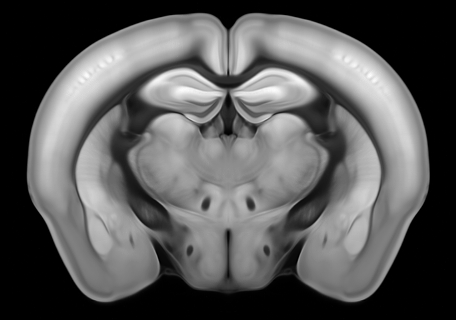
\includegraphics[width=.9\linewidth]{figures/avgt_coronal.png}
		\caption{Average coronal}
		\label{fig:average_cor}
	\end{subfigure}
	\begin{subfigure}{.3\textwidth}
		\centering
		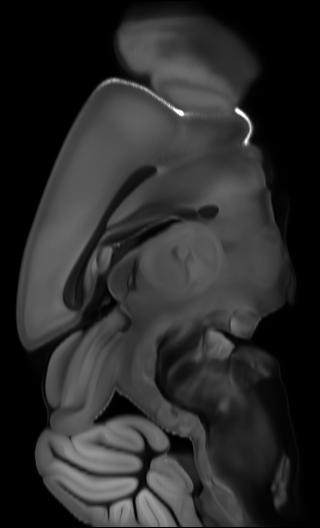
\includegraphics[width=.9\linewidth, angle=270]{figures/avgt_sagittal.png}
		\caption{Average sagittal}
		\label{fig:average_sag}
	\end{subfigure}\\
	\begin{subfigure}{.43\textwidth}
		\centering
		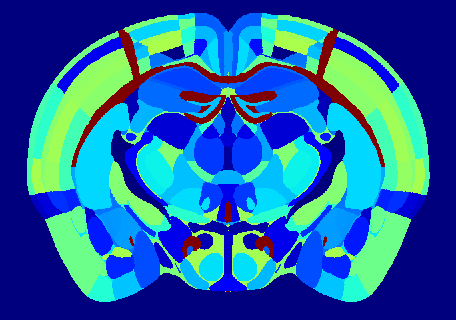
\includegraphics[width=.9\linewidth]{figures/ano_coronal.png}
		\caption{Annotation coronal}
		\label{fig:ano_cor}
	\end{subfigure}	
	\begin{subfigure}{.3\textwidth}
		\centering
		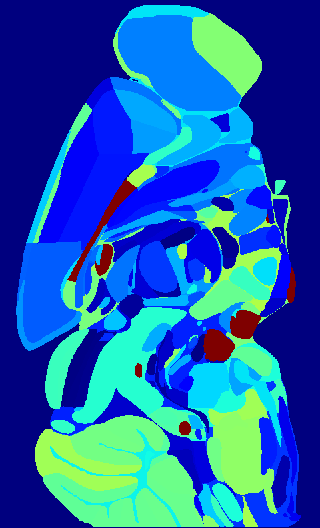
\includegraphics[width=.9\linewidth, angle=270]{figures/ano_sagittal.png}
		\caption{Annotation sagittal}
		\label{fig:ano_sag}
	\end{subfigure}\\

	\begin{subfigure}{0.9\textwidth}
		\centering
		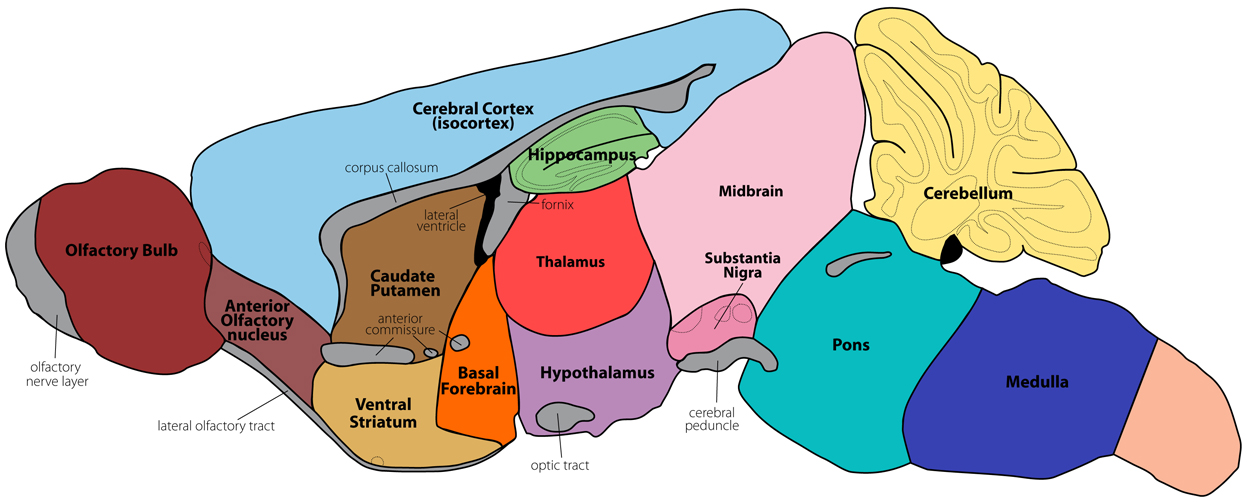
\includegraphics[width=.8\linewidth]{figures/ADULT_ATLAS.jpg}
		\caption{Mouse brain anatomy }
		\label{fig:mousebrain_anatomy}
	\end{subfigure}
	\caption[Average, annotation and anatomy atlas]{(a)-(b): Coronal and sagittal view on the ``average brain'', an averaged map of all gene expression values gathered from AMBA; (c)-(d): Coronal and sagittal view on the annotation atlas, partitioning the reference brain into $\approx900$ sub-structures; (e) Mouse brain anatomy image from the \href{http://www.gensat.org/}{gensat project} at Rockefeller University, image is licensed under Creative Commons}
	\label{fig:CCF_images}
\end{figure}

Expression values in AMBA are provided per structure as expression densities, intensities and energies. Let $g$ be the considered gene, $d$ the considered division or substructure, $P_{g,d}$ be the set of pixels within an ISH image and $P_{g,d,e}$ the set of expressing pixels, displaying expression of $g$ in $d$. Both $P_{g,d}$ and $P_{g,d,e}$ are given as measured expression intensities for the respective pixels. Thus, the three measurements are defined as shown in Table \ref{tab:expr_values}.

\begin{table}
	\renewcommand{\arraystretch}{3}
	\begin{tabular}{llp{8cm}}
		Metric name&Formula&Description\\
		\hline
		Expression density&$E_d(g,d):=\frac{|P_{g,d,e}|}{|P_{g,d}|}$&sum of expressing pixels / sum of all pixels in division\\
		Expression intensity&$E_i(g,d):=\frac{\sum_{p_e\in P_{g,d,e}} p_e}{|P_{g,d,e}|}$&sum of expressing pixel intensity / sum of expressing pixels\\
		Expression energy&$E_e(g,d):=\frac{\sum_{p_e\in P_{g,d,e}} p_e}{|P_{g,d}|}$&sum of expressing pixel intensity / sum of all pixels in division\\
	\end{tabular}

	\caption[Formulas and descriptions for the calculation of the three expression values provided by AMBA]{Formulas and descriptions for the calculation of the three expression values provided by AMBA. The respective descriptions are provided by the official \href{http://help.brain-map.org/download/attachments/2818169/InformaticsDataProcessing.pdf?version=1&modificationDate=1319667590884&api=v2}{Allen Mouse Brain Documentation}, which we note as a reference for further information on these metrics.}
	\label{tab:expr_values}
\end{table}

As expression energy provides an in-division normalization within itself, it is invariant to structure size but dependent on the actually measured intensities, it appears to be the natural choice. Expression energy was further used by all previously mentioned studies over AMBA as ground-truth; we will hence do likewise, and thus use expression value and expression energy interchangeably.

We perform a gene-set enrichment analysis (GSEA) on the expression values. GSEA is a method facilitating recognition of classes that are expressed frequently, and thus may be over-represented in the expression data. We hereby follow the works of \citet{subramanian2007gsea} and \citet{kuleshov2016enrichr} for this purpose, and integrate them into our preprocessing pipeline.

With $S$ the set of structures and $G$ the set of genes, we are now able to construct a matrix $M_{GE}\in \mathbb{R}^{S\times G}$. For simplicity, we will only consider structures with at least one non-zero gene expression value and genes that have a non-zero expression energy in at least one structure. This leaves us with $|S|=843$ structures and $|G|=16679$ genes. Note further, that the measured pixel-wise intensities are not normalized and hence the matrix entries, i.e. expression energies, may not be within the interval $[0,1]$. Hence, we will first normalize the matrix. 

However, the briefly put process of normalization remains non-trivial, not within its computational complexity, but within its neuro-biological implications and constraints. More specifically, there may be ``effective'' and ``ineffective'' genes. ``Effective genes'' may have a high impact on other downstream processes with even a few low expression intensities on one side, while ``ineffective'' genes have low impact albeit high expression intensities and high spread among the considered substructure. Summing up, the expression entries in $M_{GE}$ may not be proportional for its actual importance. 

An example may be genes describing and piloting cell proliferation. As cell division is naturally lowered in brains, in comparison to e.g. bone marrow, due to the density of neural cells, those genes may not be expressed as much. A significant increase may hence indicate a functionally deviant purpose or even pathological, i.e. cancerous, tissues, but works on low expression levels thus representing an ``effective'' gene. On the other hand, genes managing nutritional supply, may be highly expressed in all cells at all times, over-ruling the above ``effective gene'' in its expression intensities, hence constituting an ``ineffective'' gene.

Thus, there exist three different normalization schemes for this matrix: 
\begin{enumerate}
	\item A global normalization by dividing all matrix values by its global maximum, 
	\item a row-wise or per-structure normalization scheme, and
	\item a column-wise or per-gene normalization.
\end{enumerate}

While the global normalization remains the most common, it potentially leads to even lower values for ``effective'' and preserves over-represented and exaggerated expression energies for ``ineffective'' genes.
Further per-structure, i.e. row-wise, normalization allows for highlighting of expression values that are significantly lower or higher among a single structure. Unfortunately, a row-wise normalization scheme will not break the above bias, but migrates the issue from the global to a structure-level scale. The third normalization scheme helps us to identify values associated with a specific gene, which are highly expressed, significantly lower or higher among the samples, i.e. \textit{relative} expression intensities. This scheme helps us solving the issue of invariance to effectiveness of genes and allows for a fair representation of the transcriptome. The overall distribution of all all normalization schemes are depicted in Figure \ref{fig:global_hist} to \ref{fig:col_perc}.\\

\begin{figure}
	\centering
	\begin{subfigure}{.45\textwidth}
		\centering
		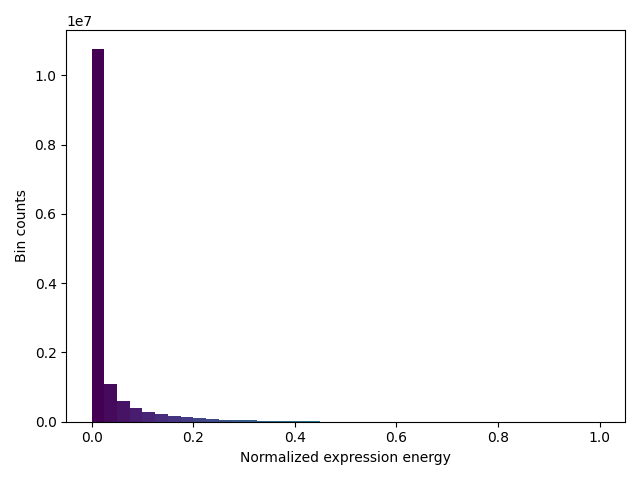
\includegraphics[width=.9\linewidth]{plotted_figures/global_normal_ge_data_histo.png}
		\caption{Histogram, global norm}
		\label{fig:global_hist}
	\end{subfigure}
	\begin{subfigure}{.45\textwidth}
		\centering
		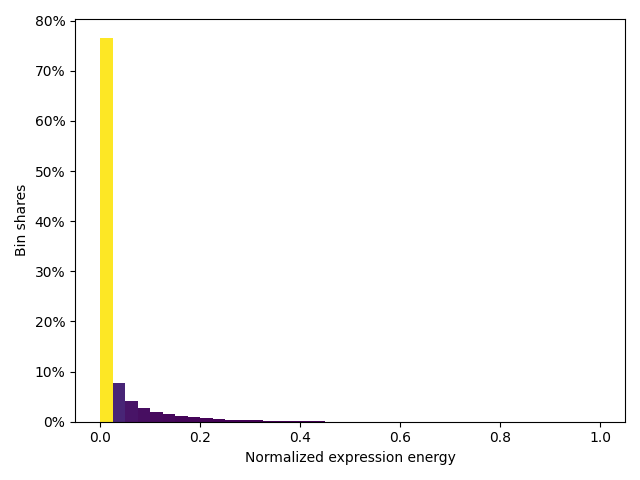
\includegraphics[width=.9\linewidth]{plotted_figures/global_percent_ge_data_histo.png}
		\caption{Bin shares, global norm}
		\label{fig:global_perc}
	\end{subfigure}\\
	\begin{subfigure}{.45\textwidth}
		\centering
		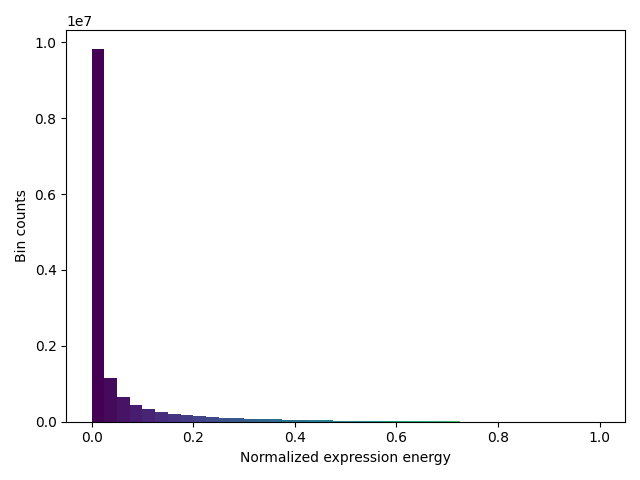
\includegraphics[width=.9\linewidth]{plotted_figures/row_normal_ge_data_histo.png}
		\caption{Histogram, row-wise norm}
		\label{fig:row_hist}
	\end{subfigure}
	\begin{subfigure}{.45\textwidth}
		\centering
		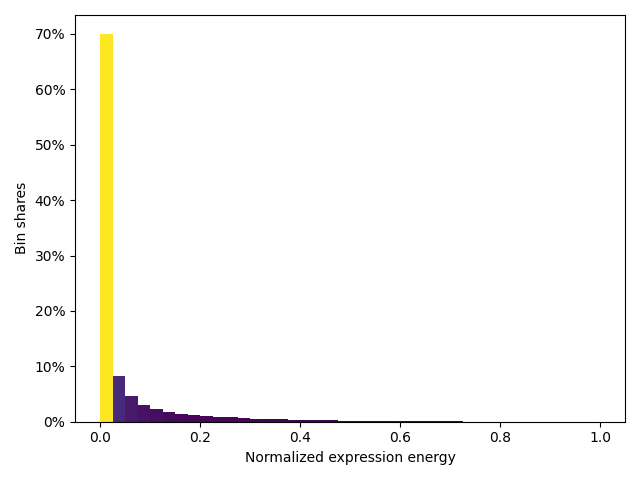
\includegraphics[width=.9\linewidth]{plotted_figures/row_percent_ge_data_histo.png}
		\caption{Bin shares, row-wise norm}
		\label{fig:row_perc}
	\end{subfigure}\\
	\begin{subfigure}{.45\textwidth}
		\centering
		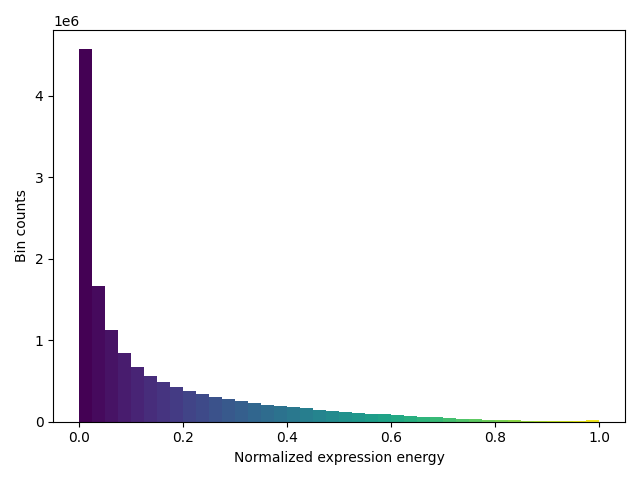
\includegraphics[width=.9\linewidth]{plotted_figures/column_normal_ge_data_histo.png}
		\caption{Histogram, column-wise norm}
		\label{fig:col_hist}
	\end{subfigure}
	\begin{subfigure}{.45\textwidth}
		\centering
		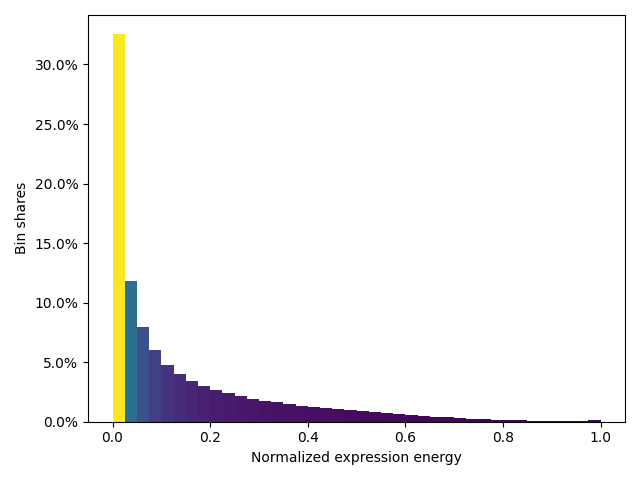
\includegraphics[width=.9\linewidth]{plotted_figures/column_percent_ge_data_histo.png}
		\caption{Bin shares, column-wise norm}
		\label{fig:col_perc}
	\end{subfigure}

	\caption[Distributions of gene expression values for the respective normalization schemes]{This figure shows the corresponding distributions of gene expression values for the respective normalization schemes, i.e. global, column-wise and row-wise, each associated with differing biologic interpretations. The expression matrix is determined by $|S|=843$ structures and $|G|=16679$ corresponding genes and the pairwise spatial gene expression values.\\ \ref{fig:global_hist}, \ref{fig:row_hist} and \ref{fig:col_hist}: Color-coded distribution of normalized expression energies; color describes the individual expression values. Note that values are on different scales i.e. $10^7$ for \ref{fig:global_hist} and \ref{fig:row_hist}, and $10^6$ for \ref{fig:col_hist}.\\ 
	\ref{fig:global_perc}, \ref{fig:row_perc} and \ref{fig:col_perc}: 
	Color-coded proportional distribution of expression energies. While showing the same distribution, colors describe the several shares of each bin. Note the different scales. We clearly see a shift of the average for the column-wise normalization in comparison to the other two approaches.}
	\label{fig:ge_hists}
\end{figure}


Especially for our binary classification task of gene expression prediction (see Section \ref{sec:probdesc_geneexp}), we need a mapping of those entries to $\{0,1\}$. Moreover, neural networks prefer inputs in the interval $[0,1]$ as we want to use $M_{GE}$ as input for the problems described in Sections \ref{sec:probdesc_dimpres} and \ref{sec:probdesc_connpred}. Thus, we threshold the resulting normalized expression energies, by applying a fixed cut-off threshold $t\in[0,1]$. We experiment with various expression thresholds as described in results Section \ref{sec:results}.

\subsubsection{Protein-protein interaction graph}
As shortly sketched in the introduction (see Section \ref{sec:introduction}), we want to apply graph convolutional neural networks over protein-protein interaction (PPI) graphs and identify patterns within. However, there are numerous databases for PPI graphs publicly and freely available.
Common sources are CPDB\cite{lo2009cpdb}, iRefIndex\cite{razick2008irefindex}, MultiNet\cite{sengupta2023multinet} and STRING\cite{STRINGv10}. Due to our experience with the database and its success in other related tasks \cite{schulte2021integration, wang2021mogonet, hinnerichs2021dti}, we will use STRING (Version 10) as ground truth data. As STRING provide probabilities and hence confidence scores for each interaction, we re-use the recommended threshold of $0.7$ in order to retrieve only high-confidence interactions. STRING database contains $300,000$ interactions between over $20,000$ genes gathered from other databases and literature for \textit{Mus musculus}. An example interaction graph for \textit{Kdm7a}, an histone demethylase required for brain development, and its interactors is shown in Figure \ref{fig:PPI_graph}.

\begin{figure}
	\centering
	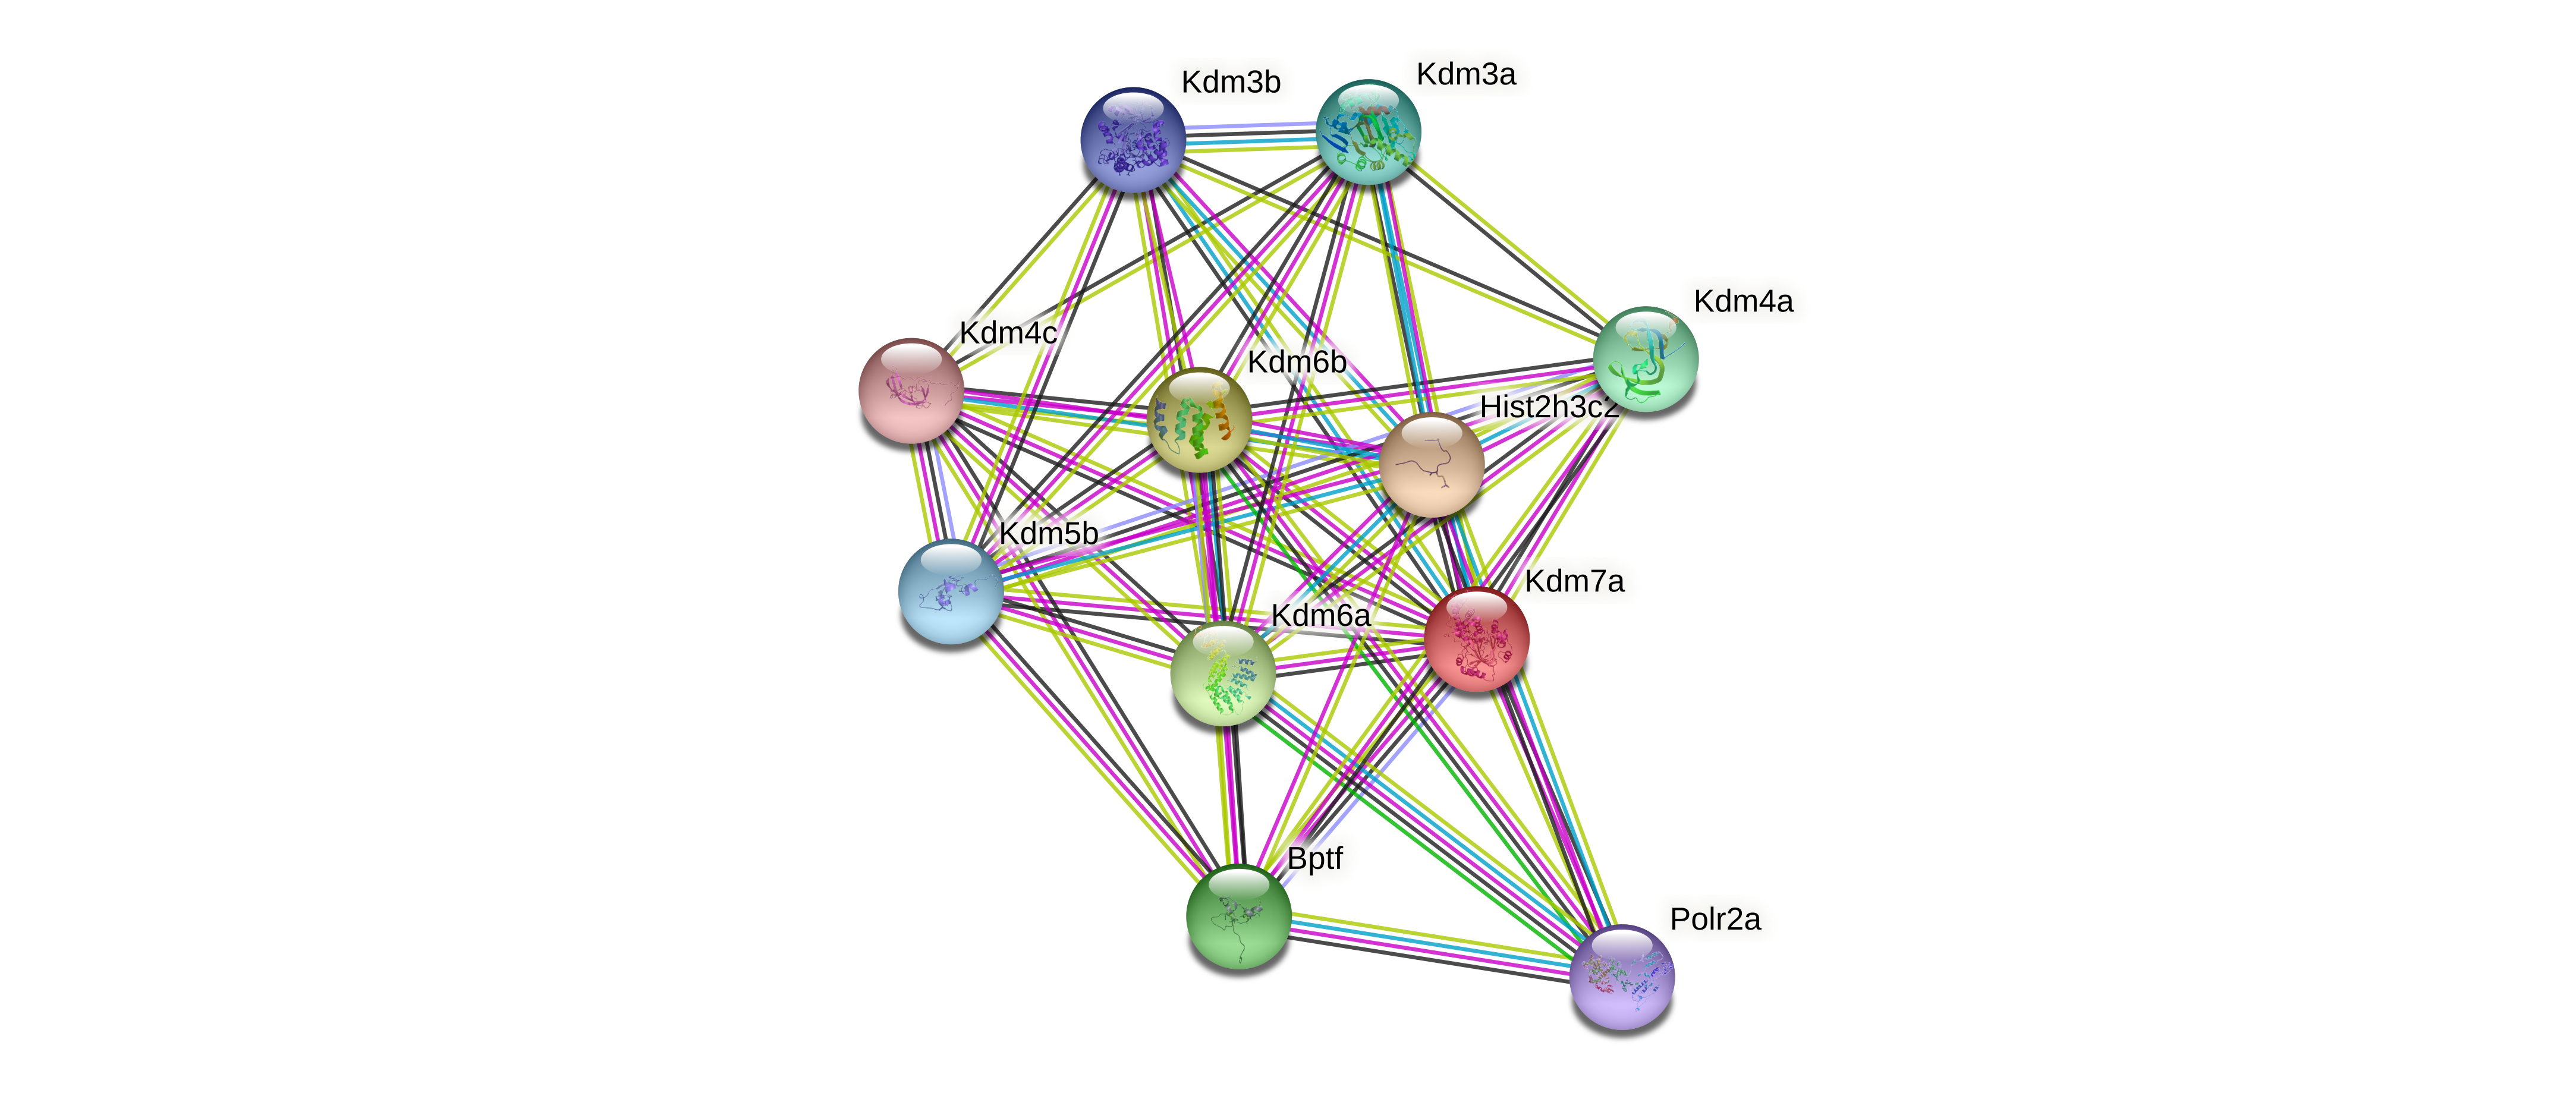
\includegraphics[width=1.\linewidth]{figures/string_hires_image.png}
	\caption[Protein-protein interaction graph for \textit{Kdm7a}]{Protein-protein interaction graph for \textit{Kdm7a}, an histone demethylase required for brain development, that is closely related to e.g. \textit{Hist2h3c2}, a protein playing central role in transcription regulation and thus proliferation activity indicating e.g. malign tumors. For more information about \textit{Kdm7a} and the used color encoding for vertices and edges, please see \href{https://string-db.org/network/10090.ENSMUSP00000002305}{string-db.org/10090.ENSMUSP00000002305}}
	\label{fig:PPI_graph}
\end{figure}

\subsubsection{Connectivity data}
Understanding neural circuits and the wiring within our brains remains an unsolved, yet fundamental task to better understand the processes of cognition. In history, there were multiple approaches to measure such brain wiring schemes. We follow the classification of ``Networks of the Brain''\cite{sporns2016networks}, distinguishing three different brain connectivities:
\begin{enumerate}
	\item Structural connectivity,
	\item Functional connectivity, and 
	\item Effective connectivity.
\end{enumerate}

The following definitions and descriptions are summarized from \citet[pp. 37-40]{sporns2016networks} as it forms the most fundamental and influential standard literature up to this date. Please see this book for further information and more in-depth analysis of this topic and their cognitive and neurological implications.\\

\textit{Structural connectivity} hereby links to physical or anatomical connections in form of linking neural elements, i.e. neurons. While this wiring measure may be relatively static on shorter time scales, ``local'' structural connectivity within regions may be dynamic or plastic over hours, days and months, due to our learning process. This is described in more detail in Section \ref{sec:struc_conn}.

\textit{Functional connectivity} (FC) tries to measure the deviation from statistical independence between distributed and often spatially remote neuronal units \cite{friston1993functional, friston1994statistical}. This data may be recorded from different sources measuring neuronal activity as elaborated further in Section \ref{sec:fun_conn}. Unlike structural connectivity, FC is highly time dependent. However, an observed statistical dependence between two nodes does not allow the inference of a causal interaction between them.

The third type of connectivity is \textit{effective connectivity}, describing the \textit{causal} effects between neural elements as detailed in \citet{friston1994functional} and \citet{friston2000attentional}. It models the actual collaboration of and dependencies between structures as noted in \ref{sec:eff_conn}.\\

\paragraph{Structural connectome data}\mbox{}\\
\label{sec:struc_conn}

We chose the AMBA partly with respect to its neat integration with the Allen Mouse Brain Connectivity Atlas (AMBCA)\cite{oh2014mesoscale}, published by the Allen institute, as a publicly available source for axonal connectivity data. The Allen Mouse Brain Connectivity Atlas is a high-resolution map of neuronal connections in the adult mouse brain, obtained from EGFP-expressing (enhanced green fluorescent protein) vectors following structural connections. As with AMBA, AMBCA tracing images were mapped back to 3D reference space using the CCF(v3) coordinates. Likewise, we are again able to group voxels to structures, parcelating the mouse brain and organized by the CCF ontology. All data was downloaded over the AllenSDK API. For a better understanding we provide a visualization of the measured EGFP data and the associated masks in Figure \ref{fig:struc_conn}.

Let $S$ be the set of structures, then $M_{\text{struc}}\in\mathbb{R}^{|S|\times|S|}$ denotes the structural connectivity matrix. We normalize all injections by their respective origin intensity projection. Second, we threshold the intensities with $t=0.1$ as the connectivity weight distribution is quite similar to AMBA (see Figure \ref{fig:ge_hists}) and eventually symmetrize the matrix. We eventually obtain $|S|=147$ structures and $\sum_{m\in M_{\text{struc}} }m=2624$ functional connections between them, depicted in Figure \ref{fig:struc_conn_vis}.


\begin{figure}
	\centering
	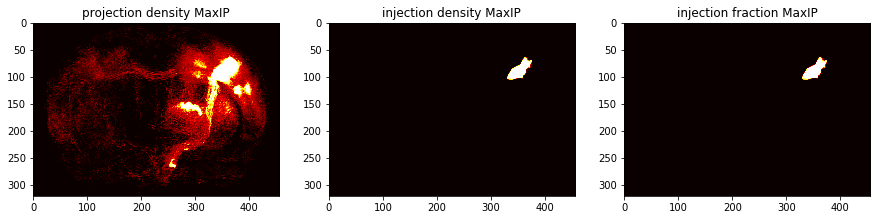
\includegraphics[width=1.\linewidth]{figures/projection_data_visualization.png}
	\caption[Raw axonal projection data derived from fluorescent proteins]{Raw axonal projection data derived from fluorescent proteins in form maximum injection projection (MaxIP) and its corresponding masks; image derived from the AMBCA pipeline. For further information please see the AMBCA documentation}
	\label{fig:struc_conn}
\end{figure} 

\paragraph{Functional connectivity data} \mbox{}\\
\label{sec:fun_conn}

The functional connectivity data was rather difficult to obtain in comparison to all other data sources. While previously described data sources are either published by the same institute or inherently provide a wide range of mappings to other databases, there are very few datasets of functional connectivity data publicly and freely available. Moreover, these rare datasets should be related to non-pathological, adult mouse brains, further diminishing resulting numbers. 

Functional connectivity may be measured using different data sources such as electrocorticography, functional magnetic resonance imaging (fMRI) or others. In most studies of this kind the latter is utilized as ground truth and thus shall be both used here and described briefly.
fMRI is a non-invasive way of detecting joint neural activity the brain. The most frequent approach is measurement of blood oxygen-level dependent signal (BOLD signal), capturing the relative levels of hemoglobin-bound oxygen in the blood. The underlying assumption presumes a correlation of used oxygen and neural activity within some given region creating a unique signal. Observation of oxygen usage hence forms an indirect and delayed measurement. Moreover, we observe all regions at the same time, while acquiring BOLD signals in response to various tasks. A temporally proximate similar characteristic signal within two regions may indicate a collaboration of those two regions for that specific task. 
However in this publication, we will focus on resting-state fMRI (rs-fMRI), where no specific task is given. This is due to the over-expression of motoric collaborations and exploration of the \textit{default mode network} \cite{sporns2016networks}. Therefore it is more reliable in the investigation of the brains hierarchy and functional organization. Hence, the additional constraint of rs-fMRI was added to the list of requirements to the dataset.\\

Nonetheless, we were eventually able to obtain resting-state, functional connectivities from AIDAmri \cite{AIDAmri2019}, publishing both their pipeline for Atlas-based Imaging Data Analysis (AIDA) and the associated dataset containing raw functional MRI data. The authors further capture the brains of 7 individuals as resting-state fMRI prior and after a stroke inducing intervention. Their follow-up software AIDAconnect (not published as a paper, please see \href{https://github.com/aswendtlab/AIDAconnect}{github.com/aswendtlab/AIDAconnect} for more information) first maps the AIDAmri data to CCF regions and second measures the associated change in both structural and functional connectivities pre and post stroke. One contribution of this work was to make this pipeline usable and provide \textit{working} scripts following their approach. We would like to thank the AswendtLab (\href{https://neurologie.uk-koeln.de/forschung/ag-neuroimaging-neuroengineering/}{Website}\footnote{neurologie.uk-koeln.de/forschung/ag-neuroimaging-neuroengineering}) for their support and help in order to get their pipeline running. 
While the authors capture axonal projections in AIDAmri, too, they measure far less structures than AMBCA on a smaller sample size, hence leading to our preference of AMBCA for this very study. \\

Let $n$ be the number of observed individuals, then $M'_{\text{func}}\in\mathbb{R}^{n\times|S|\times|S|}$ denotes the functional connectivity matrix. We threshold the pair-wise connectivity by $t=0.5$ obtaining a binary matrix. In order to combine the matrices over all individuals, we follow ``The Handbook of Functional Connectivity'' \cite{nieto2020handbook} by averaging the respective connectivities, defined by 
\begin{equation}
	M_{\text{func}}:= \left(M_{\text{func}}\right)_{i,j} = \left(\left(\frac{1}{n}\sum_{k\in [n]}M'_{\text{func}, k,i,j}\right) > t_{\text{func}}\right)_{i,j}
\end{equation}

with $>:\mathbb{R}\times\mathbb{R}\rightarrow \{0,1\} $ and $t_{\text{func}}:=0.5$. We symmetrize the resulting matrix. This leaves us with $|S|=49$ structures and $\sum_{m\in M_{\text{func}} }m=278$ connections between them. A visualization is shown in Figure \ref{fig:func_conn_vis}.


\paragraph{Effective connectivity} \mbox{}\\
\label{sec:eff_conn}

The third considered connection type is \textit{effective connectivity} describing the causal relationship between different structures. In general, effective connectivity may be derived from various neural activity data likewise to functional connectivity, i.e. fMRI data over BOLD signals or electrocorticography. As already processed and available, we use the raw BOLD signals from AIDAmri \cite{AIDAmri2019}. 
In the literature there are multiple approaches of measuring causality between signals, still constituting an active research topic. We follow the approach of \textit{instrumental variables} described in \citet{angrist2009mostly} for econometrics and famously elaborated in detail in \citet{pearl2009causality}.\\

Let $n$ be the number of individuals, then $M'_{eff}\in\mathbb{R}^{n\times|S|\times|S|}$ denotes the effective connectivity matrix. Our pipeline returns the respective pairwise beta values of each pairwise beta regression of structure related signals, which are stored in $M'_{eff}$. Beta values may be interpreted similarly to covariance matrices, whereas their magnitude and quality is more expressive. As we are only interested in the interaction itself, but not the corresponding inhibition or activation, we calculate the absolute values and normalize for each individual. Likewise to our functional connectivity preprocessing, we average the causal connections along all individuals and symmetrize the resulting matrix. This may be summarized in the following equations:
\begin{align*}
	m_{max}:=& \max \left(\left|M'_{\text{eff}}\right|\right)\\
	t_{\text{eff}}:=& 0.1\\
	M_{\text{eff}}:=& \left(M_{\text{eff}}\right)_{i,j} \\
	=& \left(\left(\frac{1}{n}\sum_{k\in [n]}\frac{\left|M'_{\text{eff}, k,i,j}\right|}{m_{max}} \right) > t_{\text{eff}} \right)_{i,j}
\end{align*}
with $>:\mathbb{R}\times\mathbb{R}\rightarrow \{0,1\} $. 
This results in $|S|=49$ structures and $\sum_{m\in M_{\text{eff}} }m=492$ causal connections between them. A visualization of measured \textit{effective connectivities} is shown in Figure \ref{fig:eff_conn_vis}.

\begin{figure}
	\centering
	\begin{subfigure}{.3\textwidth}
		\centering
		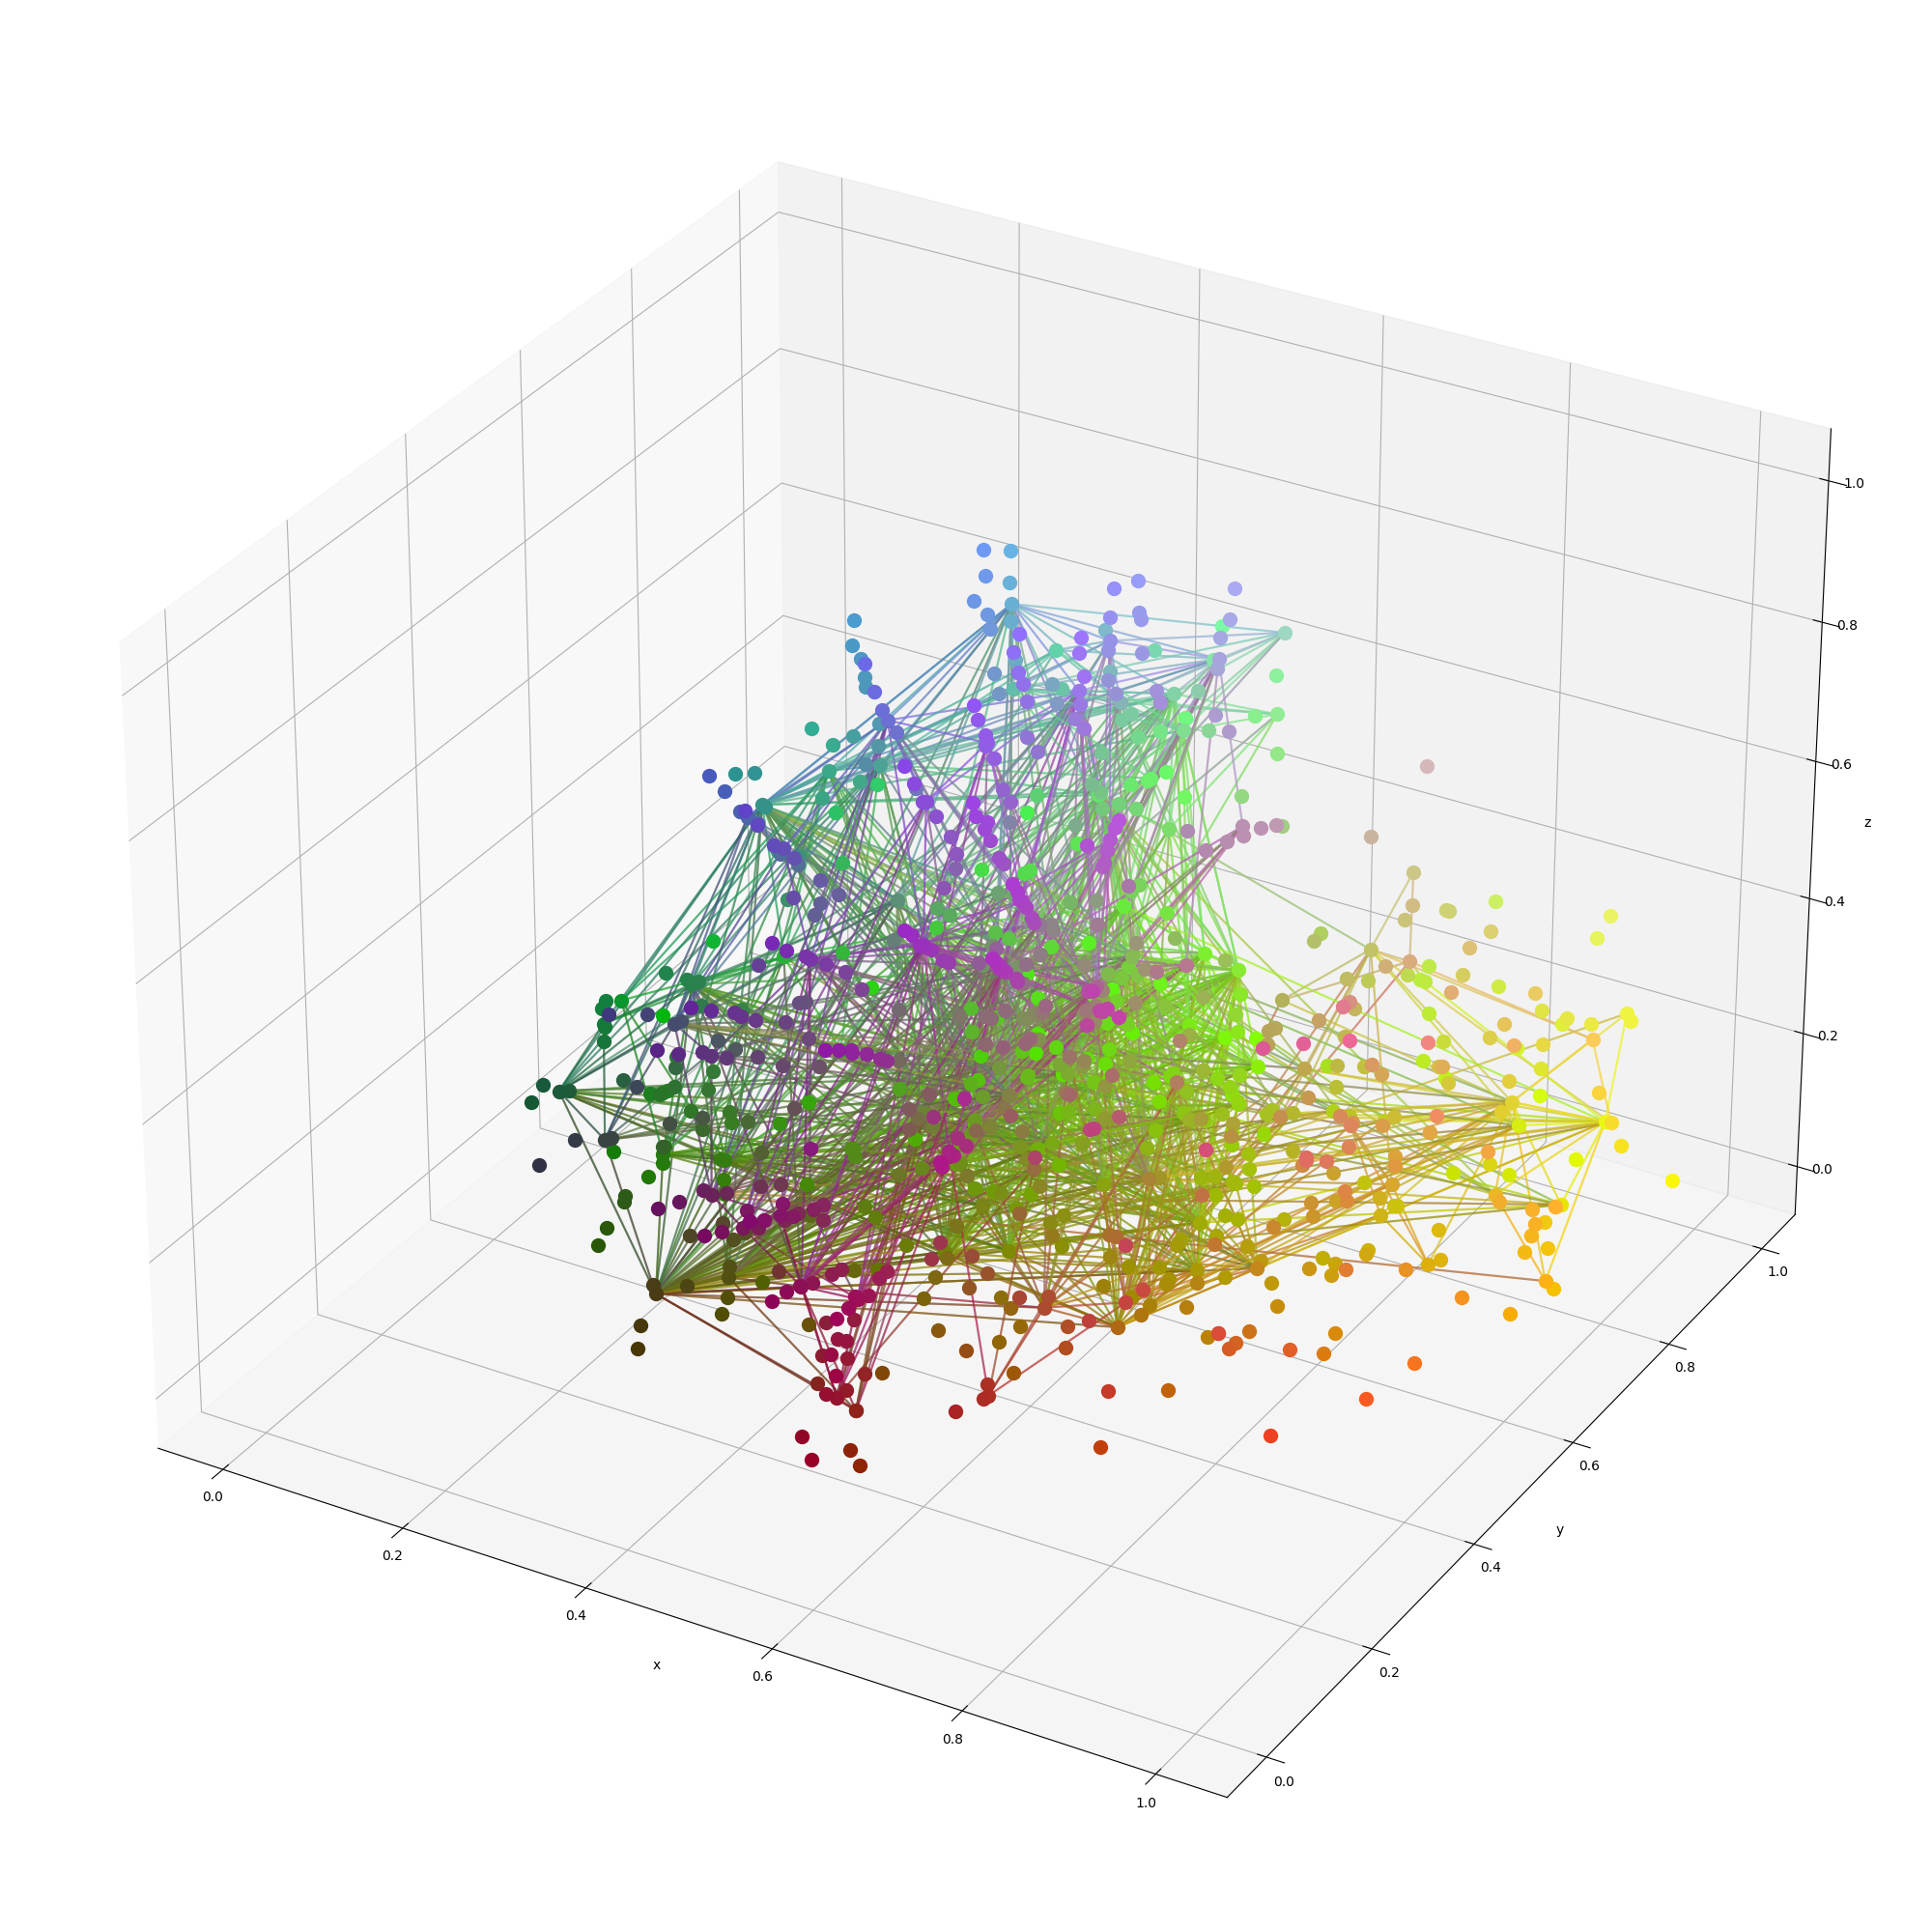
\includegraphics[width=.9\linewidth]{plotted_figures/struc_3d_conn_plot.png}
		\caption{Structural connectivity}
		\label{fig:struc_conn_vis}
	\end{subfigure}
	\begin{subfigure}{.3\textwidth}
		\centering
		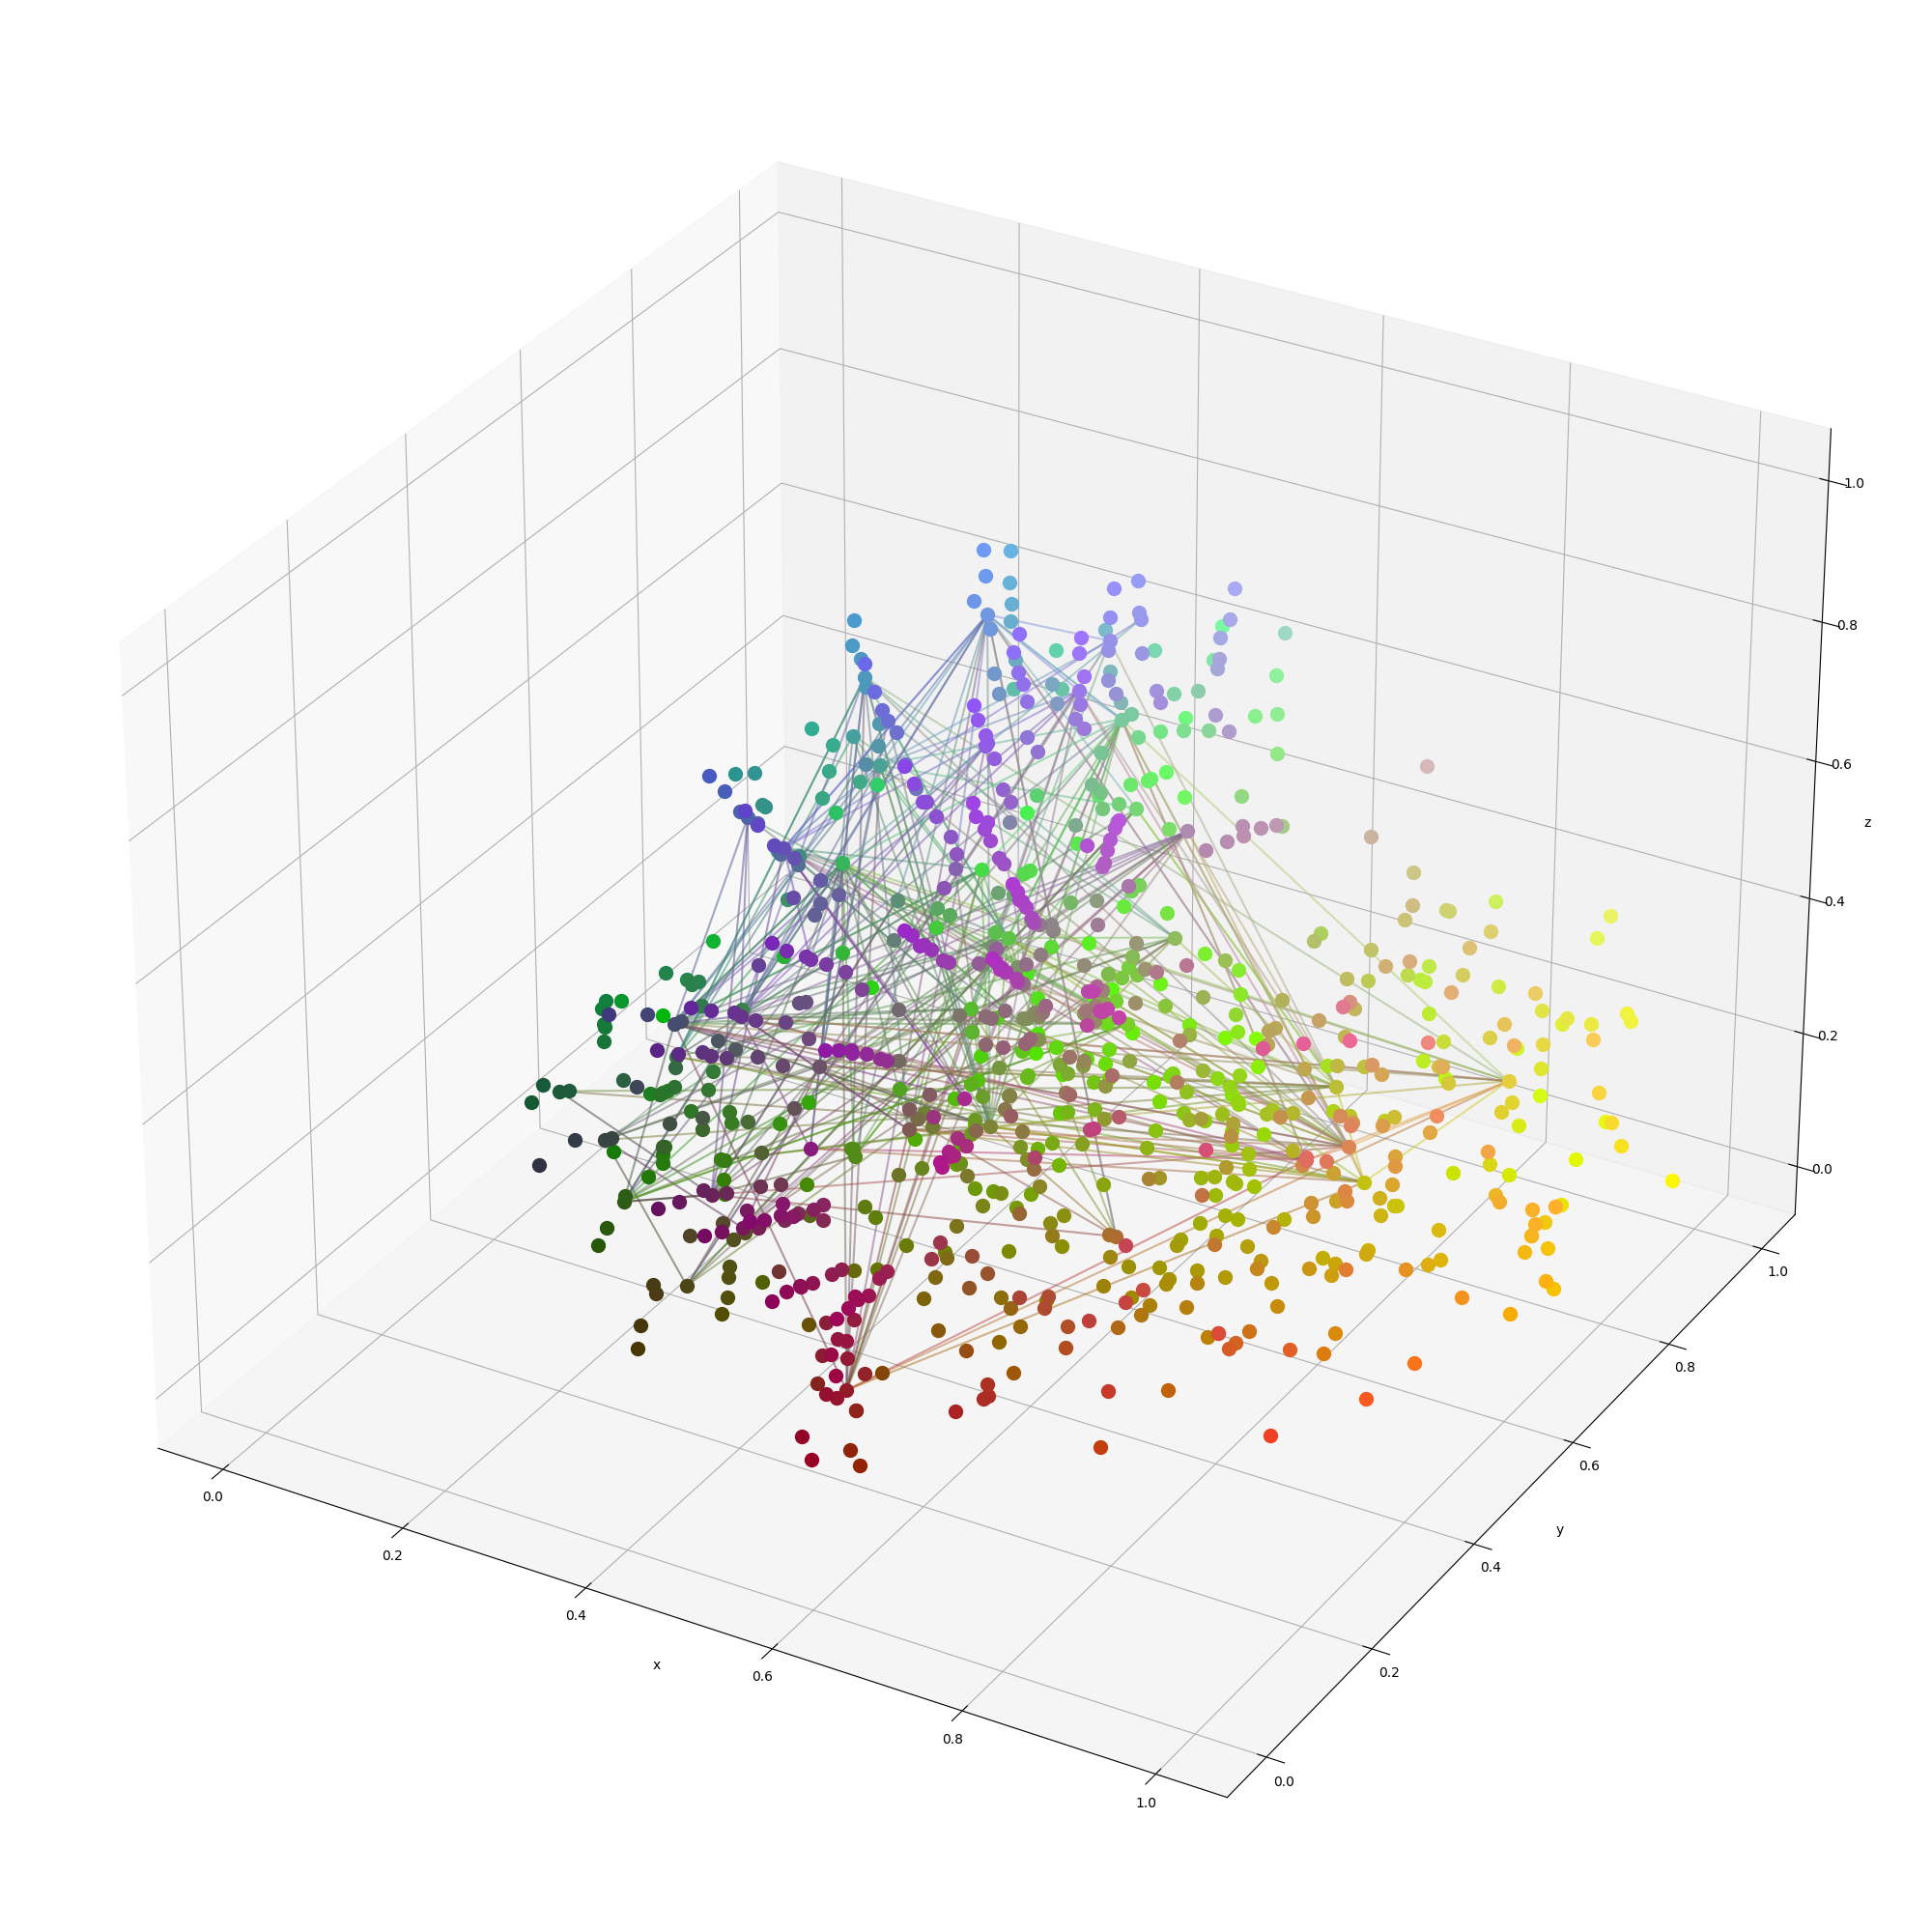
\includegraphics[width=.9\linewidth]{plotted_figures/func_3d_conn_plot.png}
		\caption{Functional connectivity}
		\label{fig:func_conn_vis}
	\end{subfigure}
	\begin{subfigure}{.3\textwidth}
		\centering
		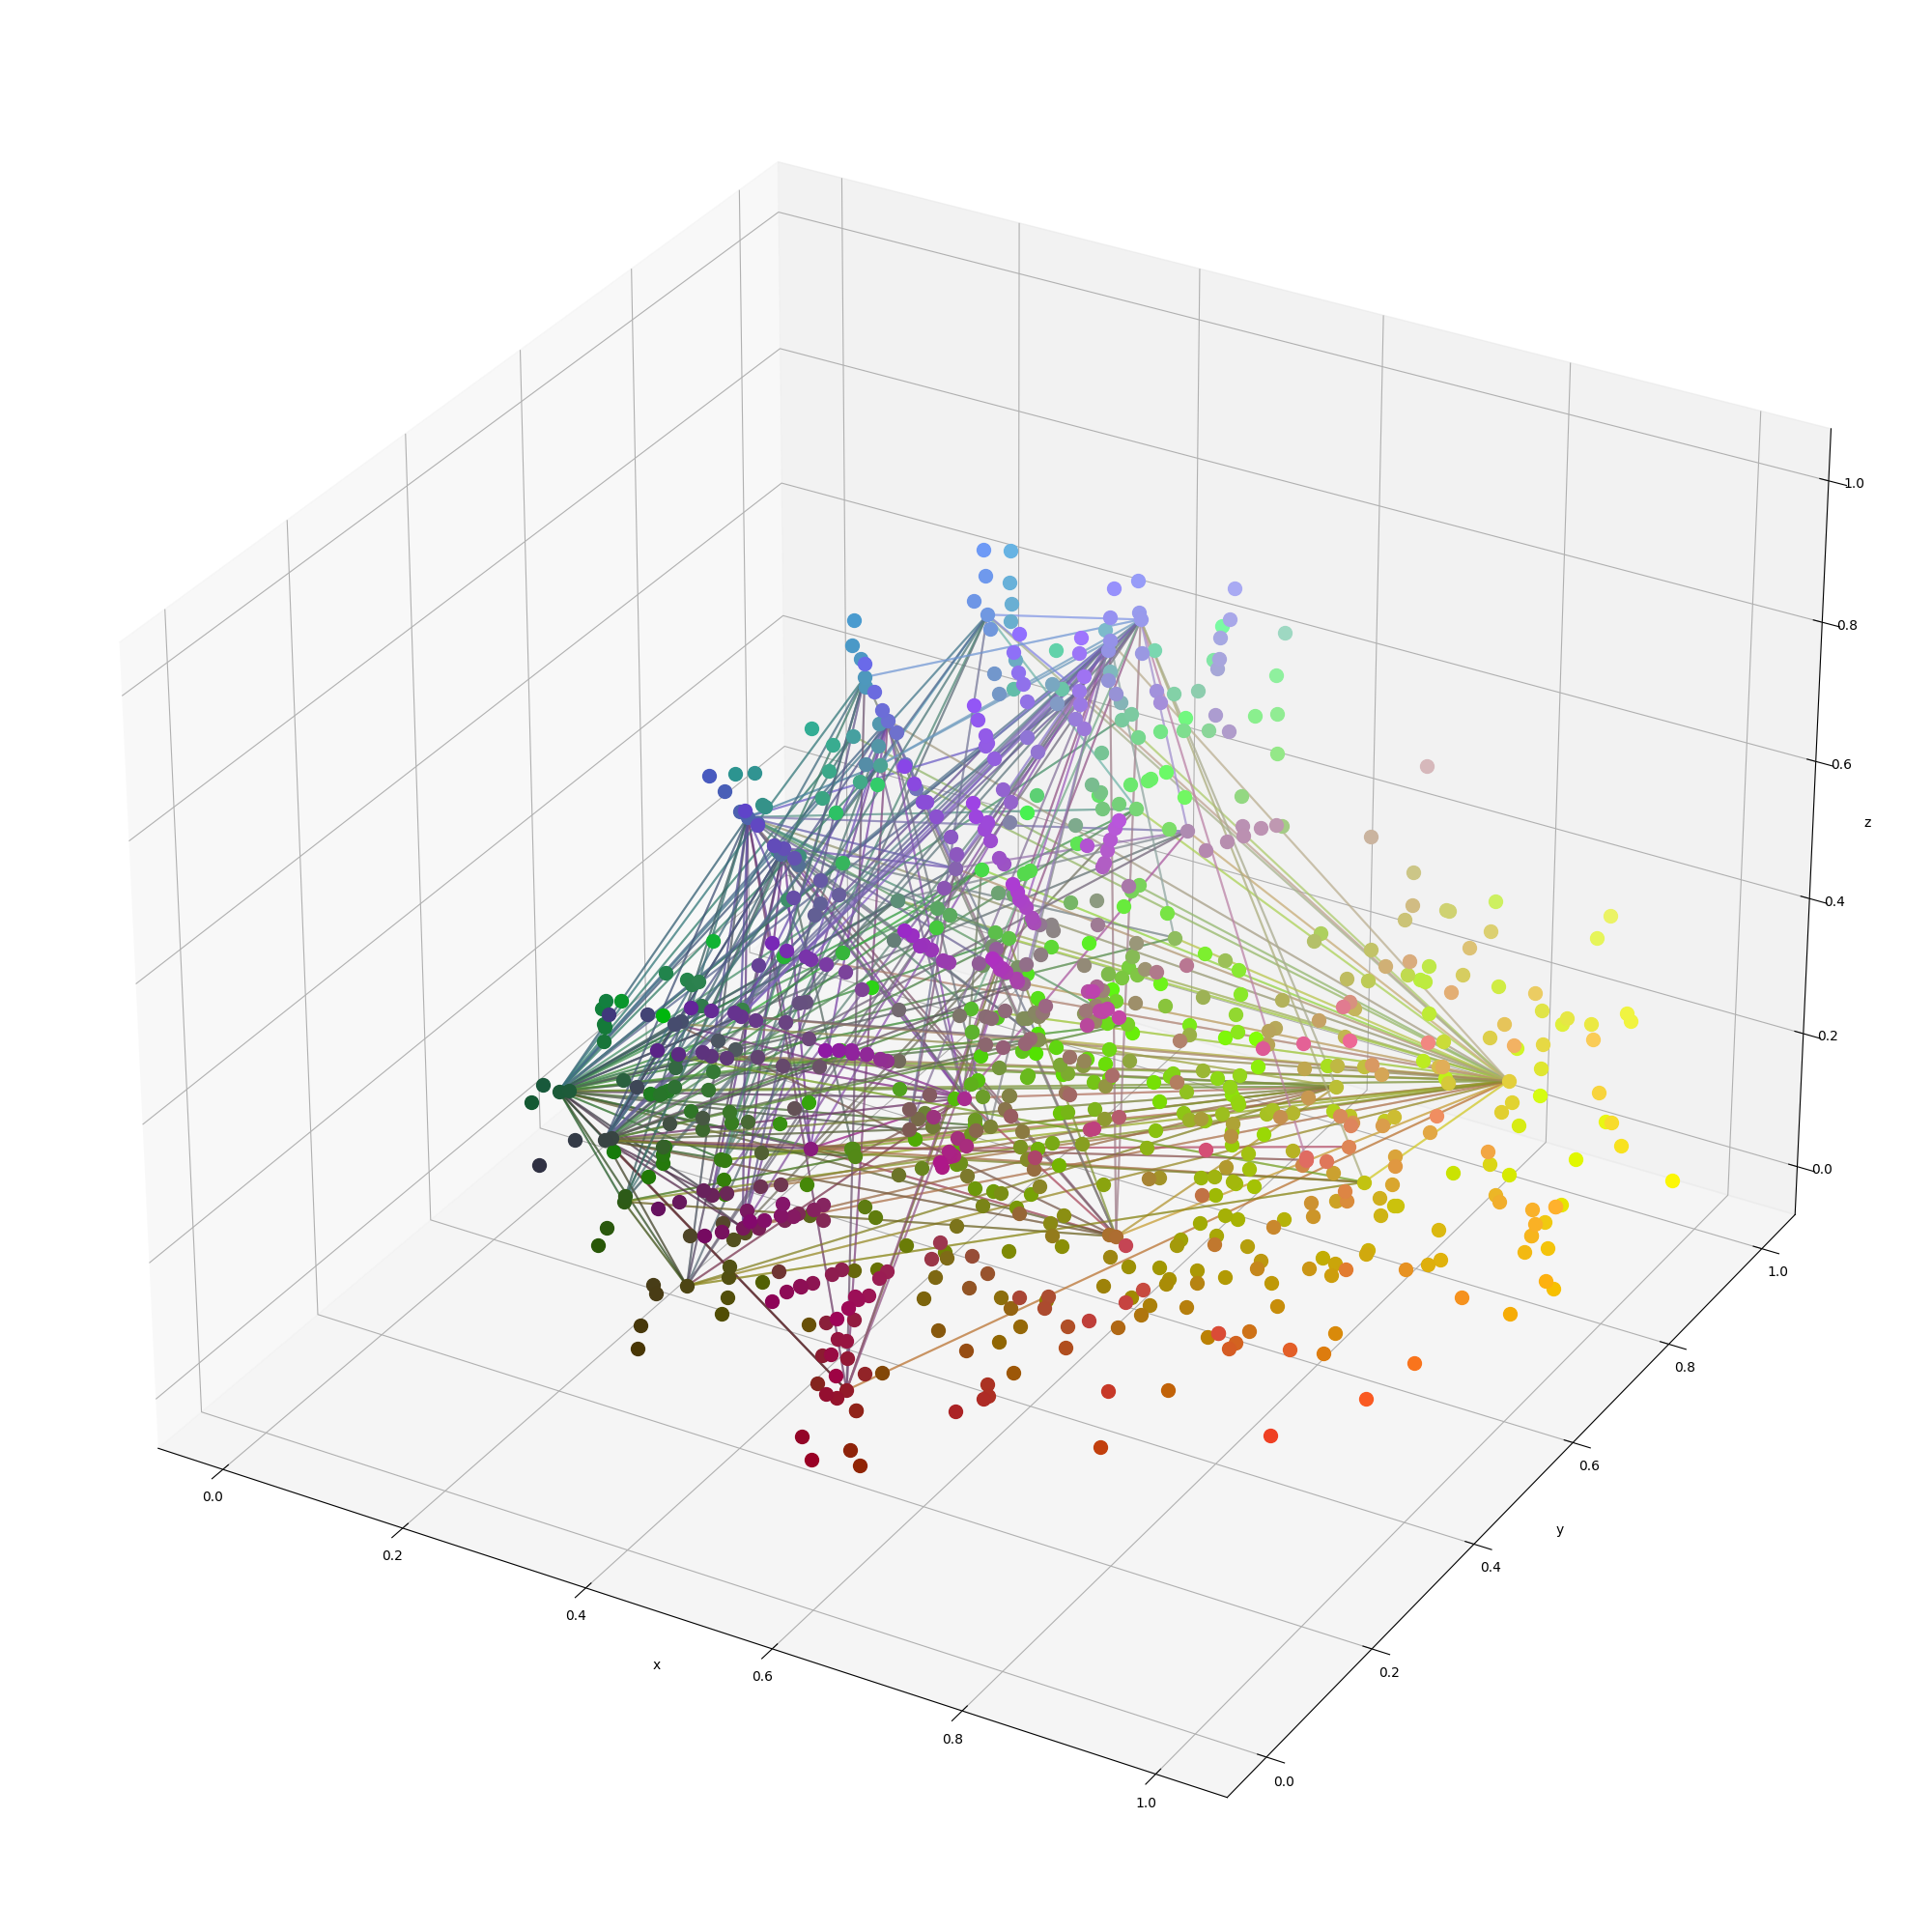
\includegraphics[width=.9\linewidth]{plotted_figures/eff_3d_conn_plot.png}
		\caption{Effective connectivity}
		\label{fig:eff_conn_vis}
	\end{subfigure}

	\caption[3-dimensional visualizations of mouse brain connectivities]{3-dimensional visualizations of mouse brain connectivities. All structures are represented by their respective center of gravity in 3D coordinates, which also describes each nodes color coding; connectivities are colored by their respective center of mass mapped into color space, too, for better visualization of depth. Statistics on this visualizations are stated in Table \ref{tab:conn_overview}.}
	\label{fig:conn_vis}
\end{figure}

\begin{table}
	\centering
	\begin{tabular}{lll}
		Connectivity type&Number of present structures&Number of links\\
		\hline
		Structural connectivity&147&2624\\
		Functional connectivity&49&278\\
		Effective connectivity&49&492\\
	\end{tabular}
	\caption[Overview on sizes of respective connectivity datasets]{Overview on sizes of respective connectivity datasets}
	\label{tab:conn_overview}
\end{table}

\subsection{Model}
\label{sec:modeldesc}

\subsubsection{Feature generation and protein representation}
\label{sec:feature_gen}
For the prediction gene expression values in the first task (see Section \ref{sec:probdesc_geneexp}), we need embeddings of each gene potentially representing its role in downstream tasks. Hence, we decided to exploit protein-function data based on both bottom-up, i.e. founded on molecular properties and associations, and top-down, i.e. starting from observable characteristics, in form of molecular and phenotypical background data. For the bottom-up representations we utilize the DeepGOPlus \cite{DeepGoPlus} embeddings, that are based on a prediction of protein-functions based on their corresponding amino-acid sequence. For top-down and phenotypical features, we use DL2vec \cite{DL2vec2020} over PhenomeNET\cite{PhenomeNET2011} an aggregation of various ontologies such as Gene Ontology (GO) \cite{GOoriginal2000, GOrecent2020}, Mammalian Phenotype Ontology (MPO) \cite{MP2009} and Uberon \cite{mungall2012uberon}, a multi-species anatomy ontology. DL2vec hereby formulates random walks over these ontologies, interpreted as knowledge graphs, and embeds them under usage of Word2Vec \cite{Word2vec2013}. 

For the other two tasks (see Section \ref{sec:probdesc_dimpres} and Section \ref{sec:probdesc_connpred}), we will use the raw gene expression values parsed from AMBA to represent each substructure.

\subsubsection{Graph convolutional neural networks}
\label{sec:graphconv}
Graphs are one of the most expressive and common data structures for structured data. Especially in bio- and neuroinformatics, pairwise relations like in protein-protein interaction graphs, molecular graphs, biomedical ontologies, and biochemical knowledge graphs are widely spread. Considering graphs we distinguish between various types that allow application of differing algorithms. Especially with respect to the four graphs mentioned in Section \ref{sec:datasets}, we will provide a brief classification.\\

\begin{mydef}[Homogeneous Graph]
	A (homogeneous) graph $G$ is given by as tuple $G:=(V,E)$ with $V$ the set of vertices and $E$ the set of edges. A graph $G$ is called
	\begin{itemize}
		\item  \textbf{directed} if $E\subseteq V\times V$, and
		\item \textbf{undirected} if $E\in 2^V$.
	\end{itemize}
\end{mydef}

Variations of graphs are defined in Table \ref{tab:graph_types}.\\


\begin{table}
	\centering
	\renewcommand{\arraystretch}{2.1}
	\begin{tabular}{lll}
		Graph type&Definition&\\
		\hline1.9
		(Undirected) Hypergraph&$G_H=(V,E)$&with $E\subseteq\mathcal{P}(V)\backslash\emptyset$\\
		Weighted graph&$G=(V,E,w)$& with $w:E\rightarrow \mathbb{R}$\\
		Node labeled graph&$G=(V,E,x)$&with $x:V\rightarrow\mathbb{R}^n$\\
		Heterogeneous graph&$G=(V,E,l)$&with $l:V\cup E\rightarrow L$ and labeling space $L$\\
	\end{tabular}

 	\caption{Definitions of different, used graph types}
 	\label{tab:graph_types}

\end{table}


With these formulations we are able to both classify all previously described graphs, but also formulate constraints on graphs for the upcoming definitions. While the structure--gene expression in combination with the associated CCFv3 ontology is an edge and node labeled, heterogeneous graph, the PPI graph from STRING, and all three connectivity graphs are edge-weighted, homogeneous ones. However, after our thresholding process all weights are reduced to the binary space $\{0,1\}$.\\

Graph convolutional neural networks are a geometric generalization of convolutional neural networks (CNN) commonly used over images, in order to learn generalizable kernels incorporating and learning to highlight local features. A stack of CNNs trained on cat and dog images, was shown to learn general features, such as ear and snout shapes. 
However, CNN filters have fixed geometric relations, i.e. we may always name and point at the element ``right of'' our current element within an image. Such orders among neighbors do not exist within graphs, and are even counterproductive, taking the order-invariance of the graph nature. Further, the number of neighbors for an element may not be constant in a graph, while they traditionally are within 2D- and 3D-images. Within a potential formulation of GCNs we would like to keep certain properties of CNNs, namely the ability to exploit locality, correlation of filter sizes and the considered neighborhood, learnable weights and node invariance. \\

We distinguish several tasks for GNNs based on the respective classification. Here classification may also be used for representation learning by increasing the dimensionality of the mapping image to the desired representation space dimension. 
\begin{enumerate}
	\item Graph classification - classifying a given, entire graph,
	\item node classification -  given a graph with incomplete node features, predict the labels of the missing ones, and
	\item link prediction - given a graph with incomplete adjacency matrix, predict the the missing links.
\end{enumerate}
In our formulated tasks, we are performing node classification in the gene expression example (see Section \ref{sec:probdesc_geneexp}), and graph classification in the sub-tasks described in Sections \ref{sec:probdesc_dimpres} and \ref{sec:probdesc_connpred}.

For naming convention identifying each layer type, we follow the notation of PyTorch Geometric \cite{PytorchGeometric}.

\paragraph{Graph convolutional neural layers (GCNConv)}\mbox{}\\
\label{sec:GCNConv}

The first formulation of GCNs was introduced by \citet{GCNConv} and assumes the following two properties of a graph.

\begin{enumerate}
	\item A \textit{homogeneous} graph $G=(V,E)$, with $|V|=N$ and $E$ summarized by the adjacency matrix $A\in\mathbb{B}^{N\times N}$
	\item Node features, defined by a node labeling $x:V\rightarrow\mathbb{R}^D$ with feature dimensionality $D$ summarized in the feature matrix $X\in\mathbb{R}^{N\times D}$
\end{enumerate}

We will use the protein-protein interaction (PPI) graph as underlying structure, while adding the representations reported in Section \ref{sec:feature_gen}. The PPI dataset
is represented by a graph $G=(V,E)$, where each protein is represented
by a vertex $v\in V$, and each edge $e\in E\subseteq V\times V$
represents an interaction between two proteins.\\ 

A GCN layer is defined by an update rule. Let $H^{(l)}\in\mathbb{R}^{N\times D}$ the current node representation at layer $l$, then the update rule is defined by.

\begin{equation}
	H^{(l+1)}:=f\left(H^{(l)}, A\right) \text{ with } H^{(0)}:=X
\end{equation}

The crucial step is encoded in the function $f$ and may consist of the following three sub-steps.
\begin{enumerate}
	\item Applying learnable weight matrix
	\item Propagate/aggregate features to/from neighbors using a message passing scheme, and
	\item Application of an activation function
\end{enumerate}
summarized by 
\begin{equation}
	f\left( H^{(l)},A \right) :=\sigma \left( AH^{(l)}\mathbf{\Theta}^{(l)} \right)
\end{equation}
with weight matrix $\mathbf{\Theta}^{(l)}$ of layer $l$, and $\sigma$ a non-linear activation function, e.g. \textsc{ReLU}. Here features are propagated by simple multiplication of the adjacency matrix. We will formulate more sophisticated aggregation kernels later in this chapter.\\

For comparison, CNNs we preserve so called \textit{translational invariance}, i.e. the same filter may pick up the same features from an object regardless of the position of the object within the image. We generalize this property for graphs with invariance of order among neighbors, called \textit{permutational invariance}. Further this formulation allows for locality exploitation.\\


The second crucial contribution of \citet{GCNConv} is a ``kernel trick'' allowing for vital speedup of feature propagation. The authors reformulate the aggregation in the following way. 

\begin{equation}
	H^{(l+1)} = \widehat{D}^{-1/2} \widehat{A}
	\widehat{D}^{-1/2} H^{(l)} \mathbf{\Theta}
\end{equation}
with $\hat{A} = A + I$ denoting the
adjacency matrix with added self-loops for each vertex, $D$ described by $\widehat{D}_{ii} = \sum_{j=0} \widehat{A}_{ij}$, a diagonal
matrix displaying the degree of each node, and $\Theta$ denotes the
learnable weight matrix for a given graph $G=(V,E)$.
Note that $\hat{A}$ is formulated such that nodes are also directly influenced by their own previous representation.
Naturally, the number of graph convolutional layers stacked equals the radius of
relevant nodes for each vertex within the graph.

The update rule for the respective nodes is given by a message passing scheme
formalized by
\begin{equation}
	\mathbf{h^{(l)}}_i = \mathbf{\Theta}^T \sum^{N}_{j}
	\frac{1}{\sqrt{\hat{d}_j \hat{d}_i}} \mathbf{h^{(l)}}_j
\end{equation}
where both $\hat{d}_i, \hat{d}_j$ are dependent on the edge weights
$e_{ij}$ of the graph. With simple, single-valued edge weights such as
$e_{ij}=1 \text{ }\forall (i,j)\in E$, all $\hat{d}_i$ reduce to
$d_i$, i.e., the degree of each vertex $i$. We denote this type of
graph convolutional neural layers by \textsc{GCNConv}.

In this initial formulation of a \textsc{GCNConv} the node-wise update
step is defined by the sum over all neighboring node representations. This leads to the effect of \textit{over-smoothing}, i.e. over-softening of strong signals, especially in highly connected, non-sparse graphs. Further this makes the stacking of multiple layers nearly impossible to achieve feasibility due to fading signals.\\

\paragraph{Graph attention networks (GATConv)}\mbox{}\\
\label{sec:GATConv}

A second approach to graph and geometric deep learning are graph attention networks (GAT), introduced in \citet{chorowski2015attention}. Likewise to GCNs, GATs may be formulated with the following steps:

\begin{enumerate}
	\item Application of a learnable weight matrix,
	\item an attention mechanism,
	\item a activation function to combine the attention values, and 
	\item the aggregation function.
\end{enumerate}
The crucial difference to plain GCNs lies within the second step, i.e. the graph attention mechanism. We therefore compute the pair-wise importance of node $j$'s representation to node $i$'s for all pairs $i,j$. We do so by concatenation of embeddings followed by the dot-product with a learnable weight vector with an eventual application of LeakyReLU. This process is summarized by
\begin{align}
	z^{(l)}_i:=& \text{ }\Theta^{(l)}h^{(l)}_i\\
	e^{(l)}_{ij}:=&\text{ LeakyReLU}\left( {a^{(l)}}^T \cdot \left( z^{(l)}_i \circ z^{(l)}_j \right) \right)
\end{align}

with learnable vector $a$ and edge weight $e_{ij}$, and allows for inclusion of a shared attentional mechanism $a$. The resulting pair-wise coefficients measuring the mutual importance are summarized for node $i$ among all possible neighbors $j$ using a softmax function.

\begin{equation}
	\alpha^{(l)}_{ij}=\frac{\exp\left( e^{(l)}_{ij} \right)}{\sum_{k\in\mathcal{N}(i)}\exp\left( e^{(l)}_{ik} \right) }
\end{equation}
The aggregation is then formulated as a weighted sum with above coefficients.
\begin{equation}
	h^{(l+1)}_i := \sigma\left( \sum_{j\in\mathcal{N}(i)} \alpha^{(l)}_{ij} z^{(l)} _j \right)
\end{equation}
We are further able to generalize this approach by so called \textit{multi-head attention} allowing for multiple attention vectors $a$, which are then summarized within the aggregation function by averaging over all heads. Similarly, to GCNConv we denote a single layer of GAT as \textsc{GATConv}.\\

\paragraph{Training deeper graph convolutional neural networks (GENConv)}\mbox{}\\
\label{sec:GENConv}

The propagation formulation of GCNs may be adjusted to other message passing schemes, as it suffers from the issues described in Section \ref{sec:GCNConv}. As the considered radius of influence is determined by the number of used GCNConv layers, but multiple layers hinder the network to pick up any signal. Thus, we
can rearrange the order of activation function $\sigma$, edge weight $e$, aggregation function
$\mathrm{AGG}$, and linear neural layer $\mathrm{MLP}$ with this
formulation as proposed by \cite{GENConv2020}:
\begin{equation}
	\mathbf{x}_i^{\prime} = \mathrm{MLP} \left( \mathbf{x}_i +
	\mathrm{AGG} \left( \left\{
	\mathrm{\sigma} \left( \mathbf{x}_j + \mathbf{e}_{ji} \right) +\epsilon
	: j \in \mathcal{N}(i) \right\} \right)
	\right)
\end{equation}
where we only consider
$\sigma \in \{\mathrm{ReLU}, \mathrm{LeakyReLU}\}$. We denote this layer type as \textsc{GENConv}.  While the reordering is
mainly important for numerical stability, this alteration also addresses
the vanishing gradient problem for deeper convolutional networks
\cite{GENConv2020}. Additionally, we can also generalize the
aggregation function to allow different weighting functions such as
learnable $\mathrm{SoftMax}$ or $\mathrm{Power}$ for the incoming
signals for each vertex, substituting the averaging step in
\textsc{GCNConv}. Hence, while \textsc{GCNConv} suffers from both
vanishing gradients and signal fading for large scale and highly
connected graphs, each propagation step in \textsc{GENConv} emphasizes
signals with values close to $0$ and $1$, and thus emphasizes strong negative and positive signals. The same convolutional
filter and weight matrix are applied to and learned for all nodes
simultaneously. 
We further employ another mechanism to avoid redundancy and fading
signals in stacked graph convolutional networks, using residual
connections and a normalization scheme \cite{DeepGCN2019, GENConv2020}, introducing residual blocks for graph convolution. The residual
blocks are reusable and may be stacked multiple times, allowing construction of even deeper graph convolutional neural networks. These residual blocks are composed of graph convolutional layer among other functions and hence allow for substitution of arbitrary graph layers as displayed in Figure \ref{fig:ResGraphBlock}.\\

\begin{figure}
	\centering
	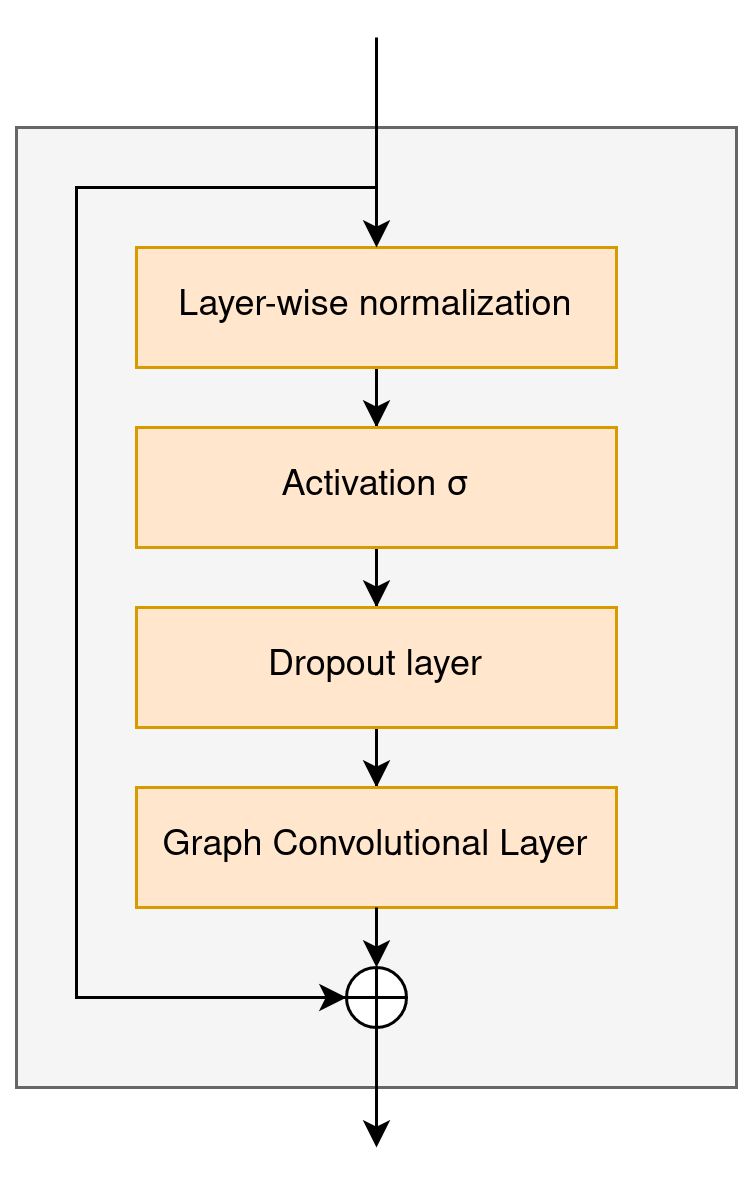
\includegraphics[width=.3\textwidth]{figures/GCN_residual_block.png}
	\caption[Residual graph convolutional blocks allowing for deeper neural networks]{Residual graph convolutional blocks allowing for deeper neural networks were proposed in \citet{DeepGCN2019} and \cite{GENConv2020}}
	\label{fig:ResGraphBlock}
\end{figure}

\paragraph{Graph kernels going beyond the Weisfeiler-Leman algorithm (KerGNN)}\mbox{}\\
\label{sec:KerGNN}

The fourth graph learning formulation, we present is \textsc{KerGNN} \cite{feng2022kergnns}. Recent studies \cite{xu2018powerful, morris2019weisfeiler} show that graph neural networks based on message passing are less expressive and powerful as the Weisfeiler-Leman (WL) algorithm \cite{leman1968reduction} and the associated WL kernel definition \cite{shervashidze2009efficient}. The WL algorithm hereby describes an isomorphism test, providing a necessary but no sufficient test for non-isomorphism, which message passing may not supersede and outperform. Thus, \citet{feng2022kergnns} provides a novel framework learning both hidden graphs combined with subgraph sampling to overcome this limitation, gaining additional expressive power. In comparison to message passing neural networks (MPNNs) which only consider \textit{subtrees}, KerGNN considers the entire induced subgraph of the respective nodes neighborhood. \\

Let $G=(V,E)$ be some graph, $\phi_{[l]}$ be the family of feature maps for each layer and $v\in V$ an arbitrary vertex. Further let $G_v=(V_v, E_v)$ be the induced neighborhood subgraph and $\phi_0$ the feature map at layer $0$ describing neighborhood mappings $\{ \phi_0(u):u\in V \}$. Then the prospective layer of the  representation $\phi_{1,i}$ depended on the $i$-th graph filter $H_i^{(l)}$ with trainable adjacency matrix $A_i^{(l)}$ is defined by

\begin{equation}
	\phi_{1,i}(v) := K\left(G_v, H_i^{(l)}\right)
\end{equation}

with random walk kernel $K(\cdot, \cdot)$ (see \citet{feng2022kergnns} for implementation details). Combined with a readout layer this may be leveraged for full graph representation learning. As we need to generate a low dimensional representations for the complete PPI graph with node features, this is naturally valuable. The readout layer is defined as a function $\Phi$ among all intermediate KerGNN layer embeddings $\phi_l$ given by 

\begin{equation}
	\label{equ:KerGNN}
	\Phi(G):= \text{concat}\left( \sum_{v\in V(G)} \phi_l(v) \text{ }\middle|\text{ } l=0,1,\dots, L \right)
\end{equation} 

with $L$ the number of stacked KerGNN layers. The authors show moreover, that this formulation is more powerful than the WL kernel and WL algorithm given a \textit{sufficient} number of stacked KerGNN layers. This draws again connections to CNNs giving a permutation invariant relation of neighbors of node $v\in V$, which e.g. GCNs are not able to derive. 


\subsubsection{Dimensionality reduction techniques}
\label{sec:dim_red}

The underlying task was briefly described in Section \ref{sec:probdesc_dimpres} with respect to gene expression. However, this task may also be formulated in a general. Here, we want to find a mapping $f_\text{emb}:\mathbb{R}^n\rightarrow \mathbb{R}^k$ with $k<n$ in order to transform data in high-dimensional space $\mathbb{R}^n$ into lower dimensionality of space co-domain $\mathbb{R}^k$, preserving \textit{meaningful properties} of the mapping's domain. The term \textit{meaningful properties} is intentionally held vague as this may refer to both domain-specific but also space specific notions. This often refers to pair-wise linkage of entities.

In domain space, e.g. biomedicine, this may refer to external graphs, such as known biological or neurological interactions and biomedical correlations between embedded entities. Space specific features rather try to preserve spatial properties of the underlying space model, e.g. euclidean space. This may be expressed in terms of maintaining local proximity, e.g. in auto-encoders \cite{ng2011sparse} or t-SNE \cite{van2008visualizing}, or retaining cluster boundaries, e.g. in support vector machines (SVMs) \cite{noble2006support}. The co-domain $\mathbb{R}^k$ of $f_\text{emb}$ is termed \textit{latent space} with latent dimensionality $k$.
In order to better understand the yielded latent space, we choose $k<4$ for a downstream, bijective mapping into color space for visualization. For our analysis we will only consider $k=3$. Note that we consider only unsupervised learning methods, as no ground truth is given for gene expression patterns and their relations.\\

We will briefly introduce all utilized dimensionality embedding methods and their respective assumptions and properties. PCA and t-SNE are not neural network-based, while UMAP and Parametric UMAP are.

\paragraph{Principal component analysis (PCA)}\mbox{}\\
\label{sec:pca}


Principal component analysis (PCA) \cite{abdi2010principal, wold1987principal} is among the most successful and simplest dimensionality reduction techniques. PCA tries to capture the data's underlying variance in space. Variance here both creates uncertainty and makes the target harder to explain and predict, but also gives a measure for importance of features. More specifically, features with no variance contain no information for the eventual embedding, similar to entropy in information theory. PCA yields a set of principal components, i.e. vectors forming a basis of the domain space, ranked by their respective variance in descending order. 

Finding such principal components is done successively for each component. This may be formulated as a linear regression problem fitting a straight line trough the data. The prospective, next components are found likewise in embedding space, after removing all data correlated to the first component, i.e. the second components must be orthogonal to the first one (or generally all preceding ones). In order to embed our domain space into three dimensions as described above, we compute the first three principal components forming a basis of the domain space. Naturally, we then express every embedding, representing entities, as coordinates of that basis. Moreover, we linearly normalize each coefficient by the respective maximum and minimum values. This is feasible as we only consider euclidean spaces, preserving the respective bases.

\paragraph{t-SNE}\mbox{}\\
\label{sec:tsne}

t-Distributed Stochastic Neighbor Embedding (t-SNE) \cite{van2008visualizing} is a generalization of Stochastic Neighbor Embedding (SNE), and often used as a direct competitor for PCA. However, as PCA only performs linear regression to build the linear basis of the respective domain space, its incapable to capture \textit{non-linear} correlations, i.e. cannot separate data that may not be separated by a plane in respective dimensionality. This issue is addressed by t-SNE and used for visualization of complex manifolds and spaces such as image representation space returned by CNNs. \\

SNE measures similarity of data points by measuring their pair-wise conditional probability describing membership to the same cluster in the supervised and neighborhood in the unsupervised learning case, and likewise for t-SNE. After construction of distributions in domain, i.e. high-dimensional, space, t-SNE's algorithm constructs similar probability distributions for in the target co-domain, i.e. low-dimensional, space minimizing the Kullback-Leibler divergence \cite{hershey2007approximating} of two points with respect to their euclidean distance in the domain space. Kullback-Leibler divergence measures pairwise divergence of two given (uni-modal) distributions $P,Q$ and is defined as relative entropy from $Q$ to $P$ by
\begin{equation}
	\label{equ:KL_div}
	D_{KL} (P||Q) := \int_{-\infty}^\infty p(x)\log \left(\frac{p(x)}{q(x)}\right)
\end{equation}
for continuous spaces, where $p$ and $q$ denote the probability densities of $P$ and $Q$, respectively.

\begin{figure}
	\centering
	\begin{subfigure}{1.\textwidth}
		\centering
		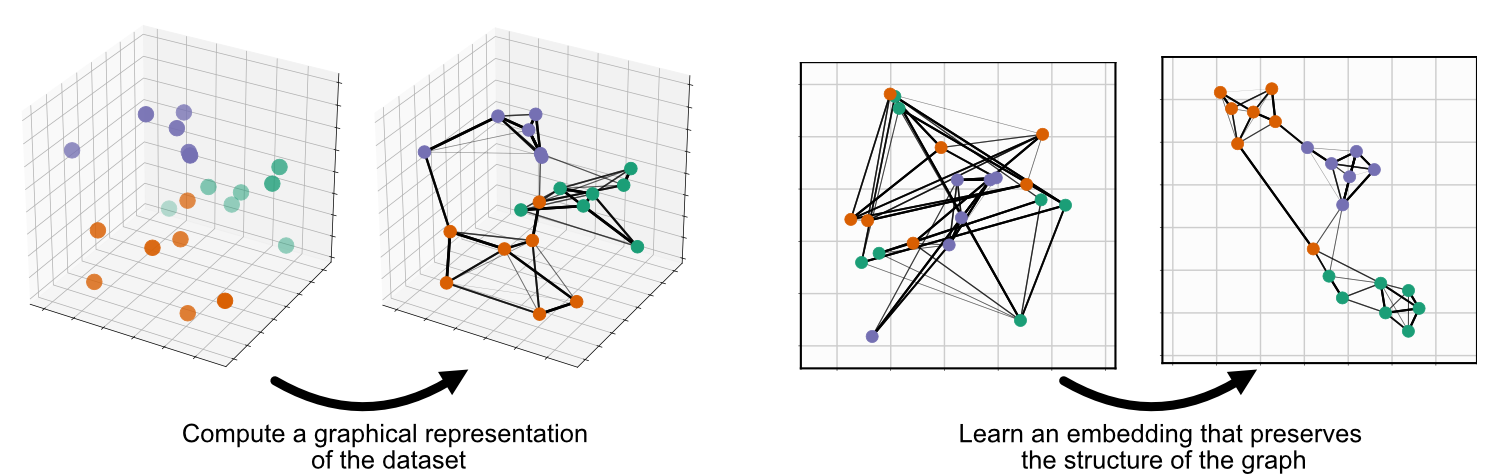
\includegraphics[width=.90\linewidth]{figures/umap-only.png}
		\caption{UMAP pipeline}
		\label{fig:umap_vis}
	\end{subfigure}\\
	\begin{subfigure}{1.\textwidth}
		\centering
		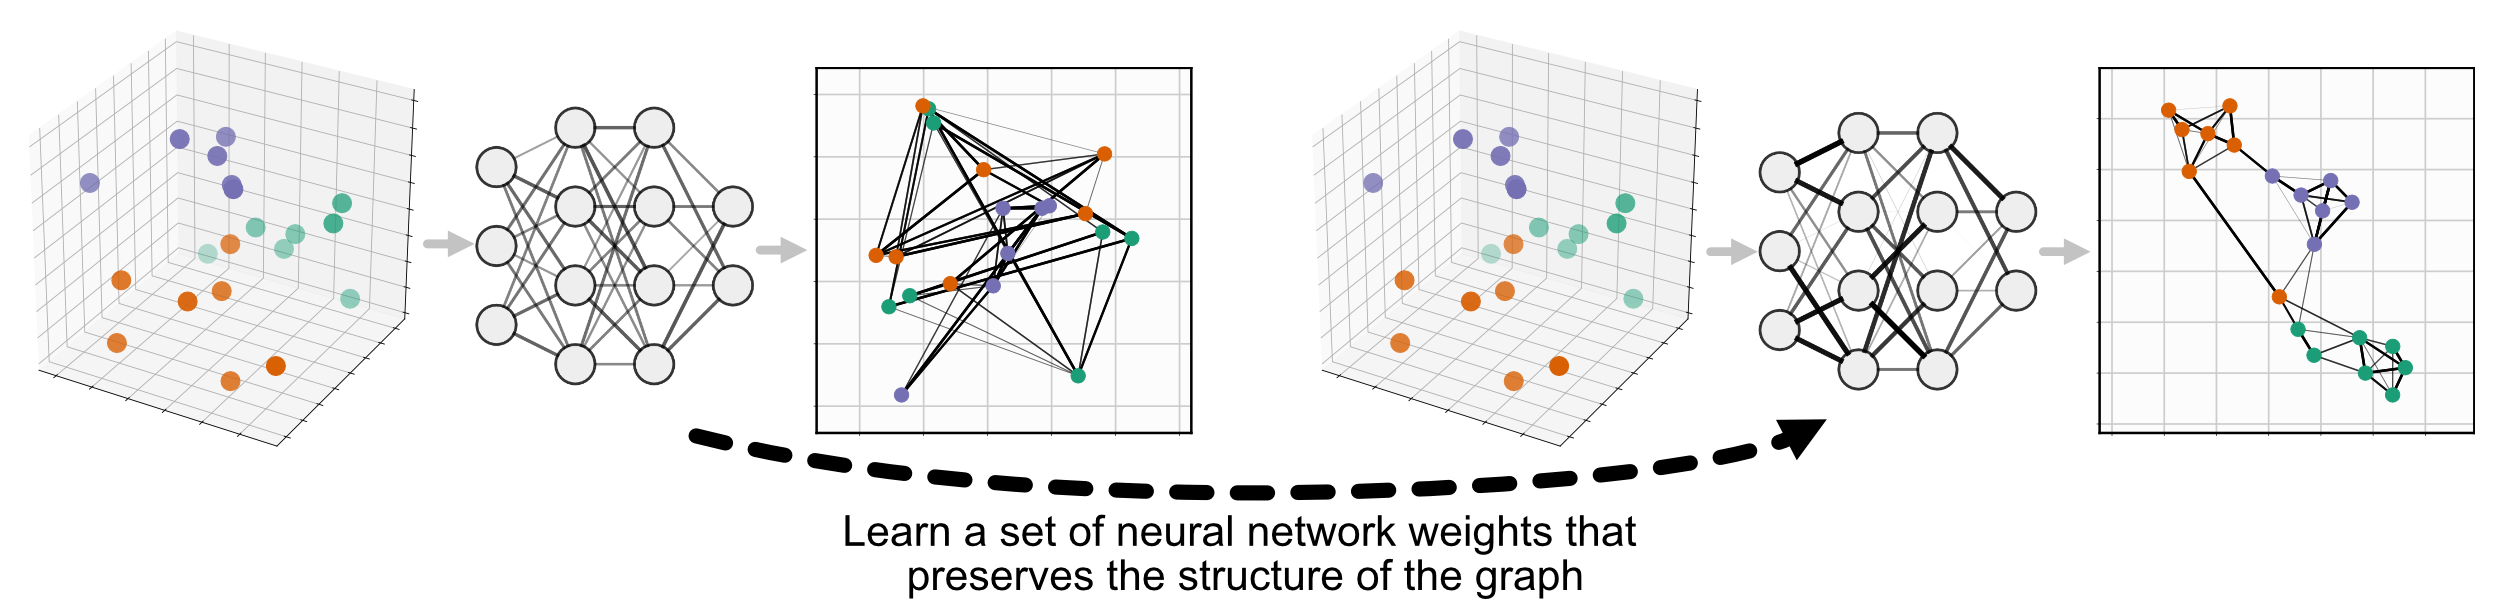
\includegraphics[width=0.90\linewidth]{figures/pumap-only.png}
		\caption{Parametric UMAP pipeline}
		\label{fig:para_umap_vis}
	\end{subfigure}
	
	\caption[Visualization of UMAP's and Parametric UMAP's respective workflows]{Visualization of UMAP's and Parametric UMAP's respective workflows. Images are taken from the \href{https://umap-learn.readthedocs.io/en/latest/parametric_umap.html}{PyPi \texttt{umap} library docs}(see \url{umap-learn.readthedocs.io}) and the papers \citet{mcinnes2018umap} and \citet{sainburg2021parametric}. The library is built and maintained by the UMAP and Parametric UMAP authors.}
	\label{fig:umap_visualizations}
\end{figure}

\paragraph{UMAP}\mbox{}\\
\label{sec:umap}

Uniform manifold approximation and projection (UMAP) \cite{mcinnes2018umap} is constructed based on and as a direct competitor of t-SNE. Likewise to t-SNE, UMAP tries to preserve the pair-wise distances, but changes the metric for distances. As described in Section \ref{sec:tsne}, embeddings are correlated with distributions and hence a distance measure over probability distributions, i.e. density functions for continuous variables as in our case, was introduced reusing the Kullback-Leibler divergence. UMAP interprets the data as samples of a an underlying manifold over Riemannian geometry-based in algebraic topology. Riemannian manifolds are embedded as a generalization of euclidean space, requiring and preserving euclidean properties only locally. More specifically, euclidean distance measures may be applied only locally. Hence, UMAP conserves euclidean distances within the fuzzy simplical complex, i.e. a ``neighborhood subgraph''.
The UMAP algorithm first computes a graphical representation of the dataset determined by an ablation of k-nearest neighbors, and learns the corresponding embeddings in a second step. \\

While this idea is very simple and na\"ive, it allows for both incorporation of neural networks for embeddings and analysis of the domain space's manifold. This approach has shown great results for a variety of tasks, which we will not cite in detail here, and especially a significant improvement over PCA and t-SNE.
A visualization of UMAP from the PyPi library umap is shown in Figure \ref{fig:umap_vis}.
A great visualization of UMAP and its expressive power especially in comparison to t-SNE is given at the \href{https://pair-code.github.io/understanding-umap/}{Google PAIR website}\footnote{https://pair-code.github.io/understanding-umap/} with loads of examples. Moreover, see \href{https://umap-learn.readthedocs.io/en/latest/performance.html}{umap-learn}'s comparison of UMAP with various other embedding methods with respect to runtime and embedding quality.

\paragraph{Parametric UMAP}\mbox{}\\
\label{sec:paraumap}

The fourth presented dimensionality reduction method is Parametric UMAP \cite{sainburg2021parametric}, that forms a direct successor of UMAP, not only by name. Developed in the same research group, UMAP learns a low-dimensional embedding of the underlying neighborhood graph in its second step, as described in Section \ref{sec:umap}. Within Parametric UMAP, this second step is substituted by neural network learning the correlation and relation of data and embeddings. This trick makes the method applicable to arbitrary deep learning applications, and enhances performance. The workflow of Parametric UMAP is shown in Figure \ref{fig:para_umap_vis}.

\subsubsection{Hyperparameter tuning}
\label{sec:hyperparameter_tuning}
As for the two classification tasks, namely gene expression prediction (see Section \ref{sec:probdesc_geneexp}) and connectivity prediction (see Section \ref{sec:probdesc_connpred}), positive links are scattered and few, training and testing datasets are highly imbalanced. Exact number may be seen in the respective dataset description sections.
The values

\begin{align}
	\label{equ:loss_weight}
	w_\text{geneexp}:=&\frac{|S| \cdot |G|}{\#positives} > 10 \text{, and}\\
	\label{equ:loss_weight_conn}
	w_\text{connpred}:=&\frac{|S| \cdot |S|}{\#positives} > 5
\end{align}

describing imbalances within the gene expression and connectivity prediction dataset hence need a suitable compensation in the respective loss functions and the evaluation metrics. Thus, we formulate a weighted version of the binary cross-entropy described by

\begin{equation}
	l(x,y):= -w\cdot\left( y\cdot \log x + (1-y)\cdot\log(1-x) \right)
\end{equation}

for given prediction $x$, ground truth $y$, and weights $w$ as described in Equations \ref{equ:loss_weight} and \ref{equ:loss_weight_conn}, respectively. The losses are averaged among all predictions in the training set on which we apply the \textit{Adam} optimizer \cite{Adam2014}, guided by an early stopping scheme. For both prediction tasks we run a 5-fold cross validation for statistical robustness.\\

We determine the optimal hyperparameters by a manual grid search among the search space, guided by the corresponding AUROC scores among the validation set. We further optimize the layer types, model depth and learning rate by a manual grid search, too.\\

For the task of dimensionality reduction, we do not have access to underlying ground truth caused by the exploratory, and unsupervised nature. Corresponding loss functions are determined by each reduction method.
Thus, optimal hyperparameters of each embedding method are determined likewise by a manual grid search.

\subsection{Evaluation and metrics}
\label{sec:evalmetrics}

As mentioned, both classification datasets are highly imbalanced, while the dataset for dimensionality prediction is not bound to ground truth for evaluation. Therefor, we will treat these two problem classes separately.\\

The classification tasks already follow the guidance of the customized and adjusted loss function. However, we need other metrics for evaluation of the observed predictions. We hence use the area under receiver operating characteristic curve (AUROC) on training and validation split data.
The AUROC score is calculated by determining true positive rates at various false positive rate thresholds and use trapezoidal approximations to estimate the are under the curve. We use the widely used and open-source implementation of \verb*|scikit-learn| for that matter. We further choose the AUROC score as primary metric over measures like the area under precision recall curve (AUPRC) as AUPRC is sensitive to imbalanced datasets \cite{jeni2013facing}.\\

For evaluation of respective embeddings in the dimensionality reduction task, we use a custom metric based on similarity of embeddings for proximate and \textit{related} sub-structures. We propose \textsc{EmbSim}, a structure dependent similarity measure for embeddings. 

Let $S'$ be the set of all structures in the brain, and $f_{\text{emb}}:S\rightarrow \mathbb{R}^k ,S\subseteq S'$ be the learned embedding function, where $k$ is set to $k=3$ if not stated otherwise. We are hereby only interested in the set of structures $S\subseteq S'$ that have a an associated embedding, i.e. gene expressions values are given for all $s\in S$ but not for all $s'\in S'$. 
Further, let $s_1, s_2$ be two structures, whose embedding similarity we are trying to determine. We compute this similarity by the pair-wise cosine similarity defined by 

\begin{equation}
	sim_\text{cos}(x_1,x_2):=\frac{x_1\cdot x_2}{\max\left( ||x_1||_2 \cdot ||x_2||_2,\epsilon \right)}
\end{equation}

for embeddings $x_1, x_2$. As we only operate within the space $[0,1]$, we normalize $f_{\text{emb}}(S)$ by their maximum and minimum value along each dimension. 

\begin{equation}
	\label{equ:norm}
	norm_S(s) = \left( norm_{S,i}'(s) \right)_i
\end{equation}

and

\begin{equation}
	norm_{S,i}'(s)=\frac{f_{\text{emb},i}(s) - \min\left(f_{\text{emb},i}(S) \right)}{\max\left(f_{\text{emb},i}(S) \right) - \min\left(f_{\text{emb},i}(S) \right)} \text{,  }s\in S
\end{equation}

with $f_{\text{emb},i}$ the $i$-th dimension of $f_{\text{emb}}$. As this is only a linear transformation, this preserves the assumptions of all considered reduction methodologies.

Second, we weight these pairwise similarities by their relation, measured by the Resnik similarity \cite{resnik1995using} $sim_\text{Resnik}:S\times S\rightarrow \mathbb{R}$, a semantic similarity measure, measuring the pairwise maximum information gain in the taxonomy of the closest common ancestor. We describe proximate and related sub-structures and their pairwise anatomical proximity, via the structure ontology of CCFv3.
We further normalize these similarities by their maximum value among all structure pairs in the ontology. This measure gives us an assessment of importance of similarities for two structures. If two entities are close in the taxonomy want the metric to emphasize the correct similarity more than for distant and un-related structures.\\

Eventually, we combine these two values weighting the similarities obtained from the cosine similarity by their corresponding Resnik similarity, normalized by the sum of weights. With 

\begin{align}
	P_{\text{cos}}:=&\left( \sum_{(t_1,t_2)\in S\times S}sim_\text{cos} (norm_S(t_1), norm_S(t_2)) \right)\\
	P_{\text{Resnik}}:=&\left( \sum_{(t_1,t_2)\in S\times S}sim_\text{Resnik} (norm_S(t_1), norm_S(t_2)) \right) \cdot \frac{1}{|S|^2}
\end{align}

we can eventually define \textsc{EmbSim} by

\begin{equation}
	\label{equ:embsim}
	\textsc{EmbSim}(s_1,s_2):= \frac{sim_\text{cos}(norm_S(s_1), norm_S(s_1)) \cdot sim_\text{Resnik}(norm_S(s_1), norm_S(s_2))}{ P_{\text{Resnik}}}
\end{equation}

and \textsc{EmbVar} by

\begin{equation}
	\label{equ:embvar}
	\textsc{EmbVar}(s_1,s_2):= \frac{\textsc{EmbSim}(s_1, s_2)}{ P_{\text{cos}} }
\end{equation}

Unfortunately, \textsc{EmbSim} may be trivially bloated by constant embeddings, maximizing the pairwise similarity. 
Hence, \textsc{EmbVar} is a direct extension of \textsc{EmbSim} additionally penalizing overly-similar or even constant embeddings. We will do an extensive analysis of these measures within Section \ref{sec:results_dimred}.\\
Second, we compare the resulting colored brain images manually, and compare them via visual features. Notably this is prone to subjectiveness.
Further, for comparison of various neural network-based models fused to UMAP and Parametric UMAP, we will use the associated UMAP loss, which is invariant to model formulation but dependent on structure selection.


\newpage
\section{Results}
\label{sec:results}
In this section we briefly describe the executed experiments and report their respective results. All implementations were done in Python and are available together with the download scripts in the \href{https://github.com/neural-data-science-lab/Treasure-Gene-expression-regions}{Github repository} \footnote{\texttt{https://github.com/neural-data-science-lab/Treasure-Gene-expression-regions}}. We further applied PyTorch \cite{Pytorch} for construction of all neural network-based models and PyTorch Geometric \cite{PytorchGeometric} for all graph learning methods. All experiments are were computed with $150$ GiB of memory and two Nvidia Tesla V100 (Volta architecture). For more information on libraries, their versions and data availability, please see the mentioned Github repository.

\subsection{Gene expression prediction}
\label{sec:results_genexp}
We originally started from the per-section prediction in order to paste its performance and results to other \textit{related} structures within in the mouse brain. One approach here is to score the models ability to genearlize from one sub-structure to \textit{related} structures via ``transfer learning''. Transfer learning was successfully applied especially in image classification and learning, and describes the re-purposing of property extraction methods, trained on one domain to the target domain, re-learning the final classification layers and steps. As features in images are fairly similar, mainly described by edges, vertices, and smaller shapes, the frequently utilized prelearned convolutional neural network (CNN) filters may be to other images. This saves both computing time, resources and energy, but also makes few-shot and zero-shot learning, i.e. learning and predicting based on very few examples in comparison to the amount of the model's parameters, feasible. Further this may yield additional insights into inter-domain relations and similarity. Filters learned on e.g. dog images, may be suitable for transfer learning towards predicting cat images, due to their phenotypical and anatomical resemblance, but less appropriate and practical for returning valuable features for e.g. optical character recognition from a document. By this performance gap for the two transfer learning tasks, we may assume that cats are more similar to dogs, while letters are rather dissimilar to dogs in their set of descriptive features. \\

We hence follow a likewise approach for mouse brains divisions. First, we will predict gene expression from molecular and phenotypical features described in Section \ref{sec:feature_gen} pursuing the frameworks described in \citet{schulte2021integration} and \citet{wang2021mogonet}'s MOGONET for human tissues. Both use \textsc{GCNConv} layers for their respective forecasts, hereby achieving tremendous performances. Second, we will try to see how generalizable these filters are for mouse brain tissues and their transcriptome from one structure to proximate ones.\\

For the first setup we anticipate the gene expression within a single structure, based on the non-structure dependent meta-information, given by the protein's representations. We thus run three different setups: (1) Molecular representations, (2) phenotypical features, and (3) both combined. We thus run five different neural network compositions described by their respective graph convolutional neural layer type. We will apply all layers described in Section \ref{sec:graphconv} and a non-graph convolutional composition as baseline method described by ``flat''. Here flat NNs, include linear layers similar to the learnable weight matrix of graph convolutional neural layers, but omitting the message passing over the graph. Sections are randomly sampled from \textit{Frontal lobe}, \textit{Parietal lobe}, \textit{Occipital lobe} and \textit{Temporal lobe} (see Figure \ref{fig:mousebrain_anatomy}). The results are available in Table \ref{tab:geneexp_pred} and are based on five different sub-structures in the \textit{transcriptomic smooth}, i.e. very similar in gene expression patters, \textit{Frontal lobe}. Results within the other tissues are similarly poor. Unfortunately, due to the specificity of the tissue and approach, we found no other works as baseline for this very task within mouse brain tissue.

\begin{table}
	\centering
	\renewcommand{\arraystretch}{1.5}
	\begin{tabular}{|l|l|llll|}
		\hline
		Feature type&Flat&\multicolumn{4}{|c}{Graph Convolutional Layers}\\
		&&\multicolumn{1}{|l}{\textsc{GCNConv}}&\textsc{GATConv}&\textsc{GENConv}&\textsc{KerGNN}\\
		\hline
		Molecular features&0.65&0.64&0.63&0.63&0.64\\
		Phenotypical features&0.68&0.66&0.64&0.66&0.67\\
		Molecular + phenotypical features &0.67&0.65&0.66&0.67&0.68\\
		\hline
	\end{tabular}

	\caption[AUROC scores for singular structures within the \textit{Frontal lobe}]{AUROC scores for singular structures within the \textit{Frontal lobe}; Forecasted with different graph convolutional neural layer types over three feature setups averaged among different substructures. Molecular features from DeepGOPlus \cite{DeepGoPlus} and phenotypical features from DL2vec \cite{DL2vec2020} over PhenomeNET \cite{PhenomeNET2011}. }
	\label{tab:geneexp_pred}
\end{table}

In our experiments we generally observe a similar, but poor performance across all feature types, with a slight improvement of semantic phenotypical features over the molecular representations. Additionally, all tested graph convolutional layers and kernel types do not improve the eventual performance of this task. Contrary, GCNs over molecular features seem to worsen the predictive performance. This may be founded in the very node specific nature of our molecular representations, which may not propagate over the network. Eventually, we observe no correspondence to the learning behavior reported in \citet{schulte2021integration} and \citet{wang2021mogonet}.\\

As described, we further test the graph convolutional neural filters in a transfer learning scenario. We thus learn the filters on different \textit{related} sub-structures within the mouse brain and validate on the target structure. Likewise to the first sub-task, we analyze results for sub-structures in different compartments of the brain: \textit{Frontal lobe}, \textit{Parietal lobe}, \textit{Occipital lobe } and \textit{Temporal lobe}.
For a given structure, we define \textit{related} divisions as ``siblings'' and ``cousins'', i.e. structures connected by paths \verb*|hasParent|$^n \circ$ \verb*|hasChild|$^n$ with $n\leq2$, within the structure ontology described by the Allen Mouse Brain Common Coordinate Framework (CCFv3). 
Results for this second step are not displayed in a separate table, but may be described here in detail. Due to the high similarity between neighboring structures, results in training and validation-phase were highly similar. For $n=1$, i.e. transfer learning from sibling structures, high correlation of adjacent divisions leads to leak from training to validation datasets. This leads to arbitrary performance, determined by the networks ability to memorize the past samples, and the number of siblings in the ontology. This holds across all observed across all brain compartments.
These results are fairly different, when concerning $n=2$, i.e. cousin structures, where results were only determined by the number of neighbors. For smaller sets of relatives, especially seen in the temporal and frontal lobe, very similar behavior as for $n=1$ was observed. However, for larger sets the results tended crucially towards outcomes shown in Table \ref{tab:geneexp_pred}. This may be due to the diminishing transcriptomic similarity for larger distances within the structure ontology and the varying parcelation across brain compartments within this ontology. \\

We thus conclude that GCNs may not be able to exploit protein-protein interaction networks for gene expression prediction. This may be caused in the complicated structure and complex nature of gene expression. We elaborate further on this matter in Section \ref{sec:discussion}. Due to negative outcomes within this task and the poor performances measured among all tested feature types, we move from the prediction of gene expression towards showing the influence of transcriptomic patterns for down-stream tasks. 


\subsection{Dimensionality reduction and its combination with different graphs structures}
\label{sec:results_dimred}

In this second section we want to show and demonstrate the results of our experiments on dimensionality reduction. This section is divided into two subsections. First, we show the validity of \textsc{EmbSim} (see Section \ref{sec:evalmetrics} and Equation \ref{equ:embsim}), followed by the results of our application of graph convolutional neural networks.

\subsubsection{On the validity of \textsc{EmbSim} and \textsc{EmbVar}}
\label{sec:results_embsim}

The formulation of \textsc{EmbSim} contains various thoughts. First, we want to achieve so called \textit{sample invariance}, i.e. a metric that is invariant to the amount and selection of samples within the ontology. As our different datasets, especially in the task of connectivity prediction, only contain data on a rather small-scale subset of structures, we want to formulate a measure allowing for cross-subset comparison of embedding similarities. 
Second, we want to penalize overly-similar embeddings. Most intuitive measures, such as the sum of cosine similarities fail to address this issue. An embedding mapping all entities to the same embedding, e.g. $(0,0,0)^T$, is optimal for this kind of measurement as it maximizes the pairwise similarity and minimizes mutual distances. However, to cope with both issues and get a sufficient understanding of the underlying data, we will need both methods. Third, we naturally want our metric to correlate with our natural understanding of a \textit{good embedding}, i.e. similar embeddings for structures with similar gene expression values.\\

First, we show the sample invariance of \textsc{EmbSim}. We assume three different toy taxonomies and ontologies, describing the sample issue, all shown in Figure \ref{fig:trees}. Let $a_i $  and $b_j$ be entities of respective classes. Further, let $sim_\text{cos}(a_i, a_j)=1$ and $sim_\text{cos}(b_i, b_j)=1$ for all pairs $i,j$, describing maximum similarity within classes. However, we further assume $sim_\text{cos}(a_i, b_j)=0$ for all $i,j$. Then the smoothness functions yield the following results:\\

{
\centering
\renewcommand{\arraystretch}{1.5}
\hspace{3cm}\begin{tabular}{l|ll}
	Tree type& \textsc{EmbSim} & \textsc{EmbVar}\\
	\hline
	Balanced $5\times 5$ tree&0.89&0.94\\
	Unbalanced $2\times 8$ tree&0.91&1.00\\
	Unbalanced $1\times 4$ tree&0.91&1.00\\
\end{tabular}
}\\

As shown, both measures are invariant to sample size comparing the $2\times 8$ and $1\times 4$ trees, if and only if samples are drawn from the same distribution. However, \textsc{EmbVar} heavily drops functioning when prompted with varying number of samples, caused by the added normalization term. This may be crucial for our purpose, as number of structures are significantly decreased in the connectivity prediction example. Additionally, we see better consistency in \textsc{EmbSim} for these examples, correctly dissecting the clusters and computing persistent smoothness values. Thus, \textsc{EmbSim} is sufficient and superior when comparing embeddings over the same set of sub-structures, but also when considering different subsets.\\

\begin{figure}
	\centering
	\begin{subfigure}{1.\textwidth}
		\centering
		\begin{tikzpicture}
			\tikzset{edge from parent/.style={draw,edge from parent path={(\tikzparentnode.south)-- +(0,-8pt)-| (\tikzchildnode)}}}
			\Tree [.Root
			[.A
			[.$a_1$ ] [.$a_2$ ] [.$a_3$ ] [.$a_4$ ] [.$a_5$ ]
			]
			[.B [.$b_1$ ] [.$b_2$ ] [.$b_3$ ] [.$b_4$ ] [.$b_5$ ] ] ]
		\end{tikzpicture}
		\caption{Balanced $5\times 5$ tree}
		\label{fig:tree_balanced}
	\end{subfigure}\\
	
	\begin{subfigure}{1.\textwidth}
		\centering
		\begin{tikzpicture}
			\tikzset{edge from parent/.style={draw,edge from parent path={(\tikzparentnode.south)-- +(0,-8pt)-| (\tikzchildnode)}}}
			\Tree [.Root
			[.A
			[.$a_1$ ] [.$a_2$ ]
			]
			[.B [.$b_1$ ] [.$b_2$ ] [.$b_3$ ] [.$b_4$ ] [.$b_5$ ] [.$b_6$ ] [.$b_7$ ] [.$b_8$ ] ] ]
		\end{tikzpicture}
		\label{fig:tree_unbalanced}
		\caption{Unbalanced $2\times 8$ tree}
	\end{subfigure}	\\
	\begin{subfigure}{1.\textwidth}
		\centering
		\begin{tikzpicture}
			\tikzset{edge from parent/.style={draw,edge from parent path={(\tikzparentnode.south)-- +(0,-8pt)-| (\tikzchildnode)}}}
			\Tree [.Root
			[.A
			[.$a_1$ ]
			]
			[.B [.$b_1$ ] [.$b_2$ ] [.$b_3$ ] [.$b_4$ ] ] ]
		\end{tikzpicture}
		\label{fig:tree_unbalanced_reduced}
		\caption{Unbalanced $1\times 4$ tree}
	\end{subfigure}	

	\caption{Different toy examples ontologies for testing the validity, strengths and weaknesses of \textsc{EmbSim} and \textsc{EmbVar} in terms of structure sub-sampling}
	\label{fig:trees}
\end{figure}


In the second issue of penalizing overly similar embeddings we less considered with the choice of sub-structures, but with the properties of embeddings. Therefore, we introduce three, na\"ive baseline functions that shall serve as comparison to overcome, and proof the third point. Functions are given by their respective probability functions $p(x)$ shown in Figure \ref{fig:baseline_distributions}:

\begin{align}
	p_\text{uni}(x):=&\begin{cases}
		1 & \text{ if }x\in [0,1]\\
		0& \text{otherwise}
	\end{cases}&\\
	p_\text{dirac}(x):= &\begin{cases}
		\infty & \text{ if }x=0.3\\
		0& \text{otherwise}
	\end{cases} &\int_{-\infty}^{\infty}p_\text{dirac}(x)=1\\
	p_\text{gauss}(x):=&\frac{1}{{\sigma \sqrt {2\pi } }}e^{-\frac{(x-\mu)^2}{2\sigma^2}} &\text{ with }\mu:=0.3, \sigma=0.05
\end{align}

For all three functions, $\int_{-\infty}^{\infty}p(x)=1$ holds by their respective definitions. \\

Further, all three are to be seen as distributions for sampling of the structure's respective embeddings, that naturally do not correlate with the corresponding division's properties. Applied smoothness metrics results are shown in Table \ref{tab:dim_red_results}. Let us consider $p_\text{dirac}$ and $p_\text{gauss}$ initially, constituting baseline distributions. Per definition, the vectors sampled from $p_\text{dirac}$ are constant and thus have a mutual cosine similarity of $1$ over all possible pairs. However, as described in Section \ref{sec:evalmetrics}, we normalize all embeddings by their respective maximum and minimum values in among each coordinate with $norm_S$ (see Equation \ref{equ:norm}). As this leads to a division by 0 error, \textsc{EmbSim} and \textsc{EmbVar} are consistently not computable for these cases. 
However, $p_{gauss}$ is a more sturdy adversary for the smoothness metrics. While $p_\text{gauss}(x)>0$ across the entire domain of $x$, the distribution may not be be adjusted by $norm_S$ and hence approximately reduced to $p_\text{uni}$. The results table Table \ref{tab:dim_red_results} shows clearly, that \textsc{EmbSim} struggles to penalize the overly similar embeddings of this very distribution. On the other hand, \textsc{EmbVar} behaves nicely, showing a clear gap of smoothness in comparison to \textit{reasonable} distributions like PCA. Hence, \textsc{EmbVar} is clearly superior in penalizing overly smooth embeddings functions.\\

Third, we want the smoothness metrics to correlate with our natural understanding of good embeddings. As described in \citet{ValkShapingBrainStructure2020} and \citet{Partel2020} gene expression patterns are very similar across the frontal lobe and the \textit{Precentral gyrus}. Used distributions generate the brain colorings displayed in Figure \ref{fig:baseline_distributions}, which do not coincide with our neurological background knowledge, e.g. transcriptomic similarity in the \textit{Cerebellum} and \textit{Isocortex} (see Figure \ref{fig:mousebrain_anatomy}). We will provide the computed visualization of the \textit{proper} embedding methods later in this chapter for comparison. However, \textsc{EmbVar} weighs the smoothness of the image even higher than the generated representations from principal component analysis (PCA). This is caused by the normalization by the sum across all similarities. As random embeddings are very dissimilar, they are not penalized and even rewarded for their spread usage of the representation space. Fortunately, \textsc{EmbSim} nicely shows a significant gap between the PCA generated and uniformly sampled vectors.\\

As we see from our toy examples, \textsc{EmbSim} and \textsc{EmbVar} have differing strengths in terms of measuring, but also struggle crucially with simple and na\"ive baseline methods. To summarize, \textsc{EmbSim} differs precisely between non-similar and similar embeddings with respect to our similarity measure, but struggles to penalize overly akin and alike embeddings from semantically \textit{better} mappings. This issue is resolved by \textsc{EmbVar}, which in return fails to properly penalize overly dissimilar embedding. Thus we conclude that only both metrics combined may be sufficient to properly judge improvement over other embedding functions.

\begin{figure}
		
	\begin{subfigure}{0.3\textwidth}
		\centering
		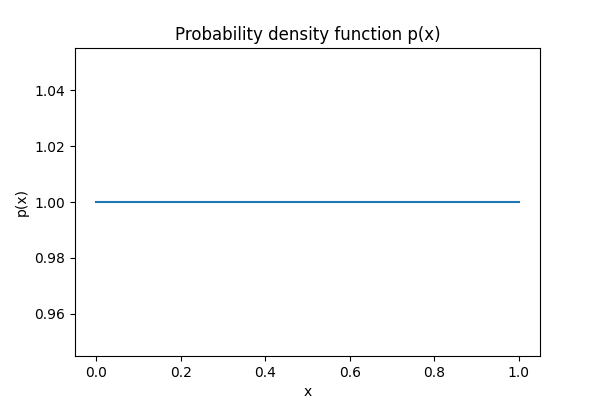
\includegraphics[width=1.1\linewidth]{plotted_figures/random_density_function.png}
		\caption{Uniform distribution $p_\text{uni}$}
		\label{fig:random_distribution}
	\end{subfigure}
	\begin{subfigure}{0.3\textwidth}
		\centering
		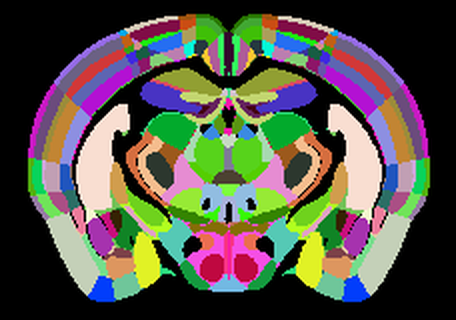
\includegraphics[width=0.95\linewidth]{../results/random_ano_coronal_50_res_slice_1.png}
		\caption{}
	\end{subfigure}
	\begin{subfigure}{0.3\textwidth}
		\centering
		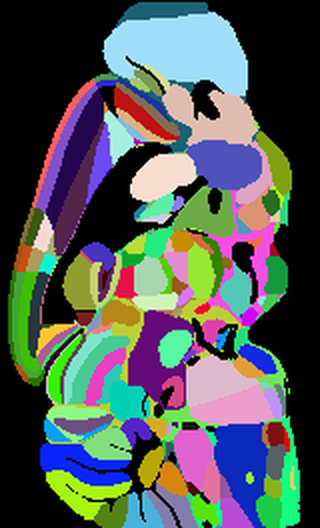
\includegraphics[width=.67\linewidth, angle=270]{../results/random_ano_sagittal_50_res_slice_1.png}
		\caption{}
	\end{subfigure}\\

	\begin{subfigure}{0.3\textwidth}
		\centering
		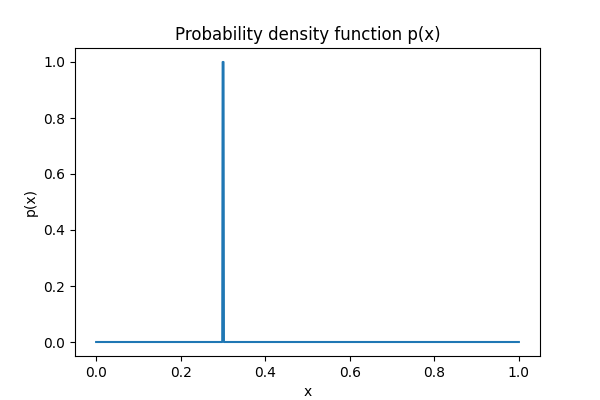
\includegraphics[width=1.1\linewidth]{plotted_figures/constant_density_function.png}
		\caption{Dirac distribution $p_\text{dirac}$}
		\label{fig:dirac_distribution}
	\end{subfigure}
	\begin{subfigure}{0.3\textwidth}
		\centering
		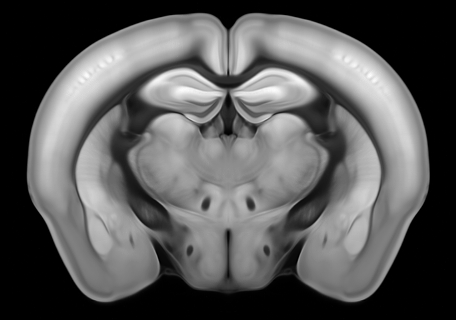
\includegraphics[width=0.95\linewidth]{figures/avgt_coronal.png}
		\caption{}
	\end{subfigure}
	\begin{subfigure}{0.3\textwidth}
		\centering
		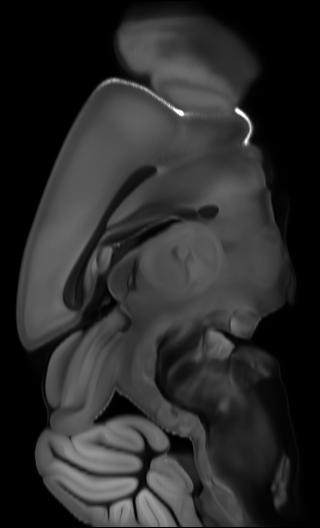
\includegraphics[width=.67\linewidth, angle=270]{figures/avgt_sagittal.png}
		\caption{}
	\end{subfigure}\\

	\begin{subfigure}{0.3\textwidth}
		\centering
		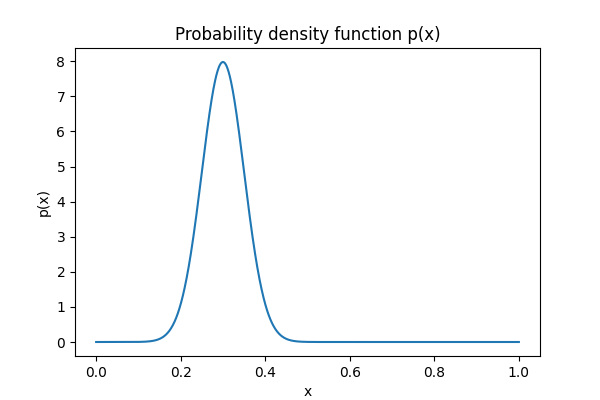
\includegraphics[width=1.1\linewidth]{plotted_figures/small_noise_density_function.png}
		\caption{Gaussian distribution $p_\text{gauss}$}
		\label{fig:gauss_distribution}
	\end{subfigure}
	\begin{subfigure}{0.3\textwidth}
		\centering
		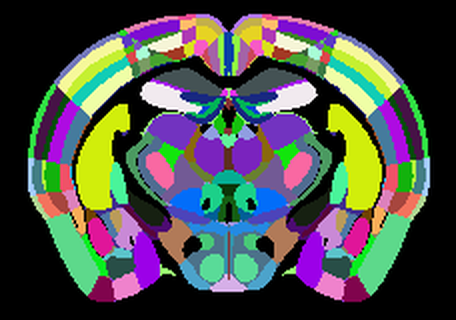
\includegraphics[width=0.95\linewidth]{../results/random_noise__ano_coronal_50_res_slice_1.png}
		\caption{}
	\end{subfigure}
	\begin{subfigure}{0.3\textwidth}
		\centering
		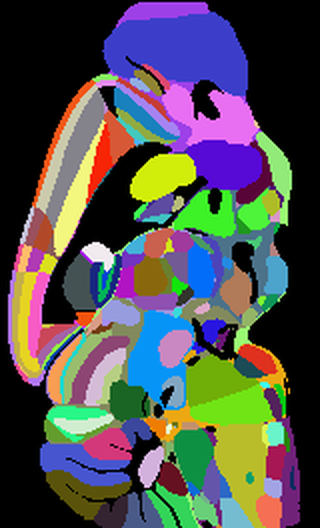
\includegraphics[width=.67\linewidth, angle=270]{../results/random_noise__ano_sagittal_50_res_slice_1.png}
		\caption{}
	\end{subfigure}\\
	\caption[Baseline functions from Section \ref{sec:results_embsim}]{Baseline functions from Section \ref{sec:results_embsim} and the corresponding colored brain structures, coronal and sagittal cross-section. (a) - (c): Uniform distribution $p_\text{uni}$; (d) - (f): Constant values with respect to Dirac distribution $p_\text{dirac}$ with peak at $t=0.3$, note that brain coloring for constant colors is not possible due to coordinate-wise normalization of embeddings, thus these images are placeholders; (g) - (i): Values sampled from Gaussian distribution $p_\text{gauss}$ with $\mu=0.3, \sigma=0.05$}
	\label{fig:baseline_distributions}
\end{figure}

\begin{table}
	\centering
	\renewcommand{\arraystretch}{1.5}
	\begin{tabular}{|l|llll|}
		\hline
		Dimensionality reduction&Uniform $p_\text{uni}$ &Constant $p_\text{dirac}$&Gaussian $p_\text{gauss}$&PCA\\
		\hline
		\textsc{EmbSim}&0.79& -- & 0.94&0.96\\
		\textsc{EmbVar}&0.99& -- & 0.91 & 1.01\\ 
		\hline
		
	\end{tabular}

	\caption{\textsc{EmbSim} and \textsc{EmbVar} scores for baseline functions, i.e. uniform, dirac and gaussian distribution, and PCA }
	\label{tab:dim_red_results}
\end{table}

\subsubsection{Enhancing neural embedding methods with GCNs}
\label{sec:results_dim_GCN}
In this section we will examine in more detail the results of our dimensionality reduction experiments. 
Thus, we first investigate the overall similarity of gene expression values across the mouse brain, measured by \textsc{EmbSim} and \textsc{EmbVar} based on the raw expression values as baseline method to overcome. We combine this with a study on the most expressive genes and the corresponding normalization scheme (see Section \ref{sec:geneexp_data}). Afterwards, we  analyze the influence of GCNs over PPI graphs on the performance and expressivity of the dimensionality reduction approaches.\\

Please note that the majority of these results are image-driven. As printed versions likely will not capture the entire color depth and nuances shown, please refer to the digital version of this script for more insights.\\

Our data preparation scheme allows for testing of different ways of representing omics data. We hence evaluated various ways to normalize gene expression values, as these normalizations capture varying biological information. Generally, there are the four possible normalization schemes possible, the three introduced and explained in Section \ref{sec:geneexp_data} and no normalization, which makes the features infeasible for the neural network-based approaches, e.g. UMAP and Parametric UMAP.
Further, we survey the behavior of dimensionality reduction methods, based on different subsets of genes. We therefor rank the genes based on their respective sum of expressions across all structures, with respect to each normalization scheme. We then select the $N\in \{20, 100, 1000, 16679\}$ most expressed genes and prune each sub-structure representation down to these genes. For a better overview we will only display the results PCA and UMAP here, but all reduction embeddings behave likewise. Results are depicted in Table \ref{tab:gen_red_baseline}. Experiments were repeated 5 times for the non-deterministic approach UMAP and averaged over all results.\\

\begin{table}
	\centering
	\renewcommand{\arraystretch}{1.2}
	
	\begin{tabular}{|ll|l|l|l|l|l|l|}
		\hline
		&&\multicolumn{2}{c|}{Raw gene expr. }&\multicolumn{2}{c|}{PCA}&\multicolumn{2}{c|}{UMAP}\\
		$N$&$norm$&\textsc{EmbSim}&\textsc{EmbVar}&\textsc{EmbSim}&\textsc{EmbVar}&\textsc{EmbSim}&\textsc{EmbVar}\\
		\hline
		\multirow{4}{*}{$20$}&none&0.91&0.99&0.94&1.00&0.96&0.99\\
		&row&0.91&0.99&0.91&1.00&0.98&0.99\\
		&column&0.94&1.00&0.95&1.00&0.95&0.99\\
		&global&0.91&0.99&0.94&0.99&0.97&1.00\\
		\hline
		\multirow{4}{*}{$100$}&none&0.90&1.00&0.95&1.00&0.95&1.00\\
		&row&0.90&1.00&0.92&1.00&0.94&1.00\\
		&column&0.91&1.00&0.95&1.00&0.91&1.00\\
		&global&0.90&1.00&0.94&1.00&0.95&1.01\\
		\hline
		\multirow{4}{*}{$1000$}&none&0.88&1.01&0.96&1.00&0.94&1.01\\
		&row&0.88&1.01&0.94&1.00&0.96&1.00\\
		&column&0.84&1.02&0.95&1.00&0.96&1.02\\
		&global&0.88&1.00&0.96&1.00&0.94&1.01\\
		\hline
		\multirow{4}{*}{$16679$}&none&0.84&1.01&0.96&1.00&0.92&1.03\\
		&row&0.84&1.01&0.94&1.01&0.93&1.02\\
		&column&\textbf{0.72}&\textbf{1.03}&\textbf{0.96}&\textbf{1.01}&\textbf{0.96}&\textbf{1.01}\\
		&global&0.84&1.01&0.97&0.99&0.92&1.03\\
		\hline
		
	\end{tabular}
	\caption[\textsc{EmbSim} and \textsc{EmbVar} scores for differing gene subsets, normalization techniques and embedding methods]{\textsc{EmbSim} and \textsc{EmbVar} scores for differing gene subsets, normalization techniques and embedding methods; Raw gene expression describes $f_\text{emb} = id $, i.e. every structure is encoded by its raw, but normalized gene expression value}
	\label{tab:gen_red_baseline}
\end{table}

There are several trends and properties clearly visible in Table \ref{tab:gen_red_baseline}. Foremost, raw gene expression values differ in their corresponding similarity measured by \textsc{EmbSim} and \textsc{EmbVar}, across the considered number of genes. The similarity is comparable to PCA and UMAP results for the subset of 20 most expressed genes. However, the low \textsc{EmbVar} value diagnoses overly similar embeddings. The more genes we consider, the more the resemblance decreases, culminating in \textsc{EmbSim}s and \textsc{EmbVar}s of 0.72 and 1.03 respectively. This indicates both the most information content, which follows naturally by the features derivation process, and spread of data. 
Moreover, we may clearly see a large discrepancy in kinship across the various normalization schemes. As described in Section \ref{sec:geneexp_data}, about 70\% of all expression values are very close to zero for none, row-wise and global normalization, leading to increased sameness in representation. \\

Fortunately, both PCA and UMAP are able to both extract the important features, but also keep the \textit{less relevant} values for spreading of embeddings along the representation space approaching a clearer dissection of clusters. Moreover, UMAP and PCA as representatives for traditional and neural network-based dimensionality reduction approaches both clearly outperform the baseline of similarity of raw gene expression values. 
This reasons and underlines our choice of normalization scheme and gene set choice, but also accentuates the validity of elected similarity metrics.\\

In the second step we approach the impact of GCNs on this embedding method. Initially, we show the computed performances across all introduced methods without GCNs, followed by a description and implementation details of the used model in combination with GCNs, and closed by their respective results and the insights we gain from this. Statistics of these trials are shown in Table \ref{tab:dim_red_GCN}. Corresponding brain images are shown in Figure \ref{fig:dim_red_vis}.\\

For our experiments we evaluate the four methods PCA, t-SNE, UMAP and Parametric UMAP on the unsupervised task of dimensionality reduction based on the raw, normalized gene expression energy data over the full set of genes. We consider 843 structures and 16679 associated genes. As mappings to the corresponding proteins are not available for all genes and some genes are linked with the same Entrez ID, we yield a total subset of 10689 genes eventually. We prune the corresponding representations accordingly for GAT-based methods, but also test for the full set of genes. Only results for the pruned set of genes are shown, as full set performances are \textit{very} similar. We further extended a digit in these results tables, to underline the rather marginal gaps measured.
We generally generally see a very solid performance across all applied methods. Moreover, all ``baseline'' methods, i.e. PCA, t-SNE and UMAP achieve akin \textsc{EmbSim} and \textsc{EmbVar} scores. A noticeable drop in both measures and the UMAP-loss is observed from UMAP to Parametric UMAP. For these experiments we tested numerous hyperparameter settings, as described in Section \ref{sec:evalmetrics}. Their corresponding images may be see in Figure \ref{fig:dim_red_vis}. We thus map the corresponding embeddings into color space and display a coronal and one sagittal cross-section across the colored CCFv3 reference atlas. For a better intuition about measured section boarders, please refer to Figure \ref{fig:baseline_vis}. 
Here PCA and t-SNE show a very diverse spectrum, causing the high performance with respect to \textsc{EmbVar}. Moreover, the corresponding images are highly parcelated and boarders between neighboring structures are clearly visible. This lacking smoothness of embeddings may also be seen in the 3D-scatter plot, which we will not display in this publication due to lack of additional insights. \\

This issue is solved with the formulation of UMAP as described in more detail in Section \ref{sec:dim_red}, ensuring smoothness and closeness of similar embeddings. This is clearly visible in Figure \ref{fig:UMAP_cor} and \ref{fig:UMAP_sag}. Both coronal and sagittal cross-section greatly improve the smoothness of embeddings across structures, while clearly highlighting the overall regions. However, we evidently detect the issue of over-smoothing, which we could not fix with different sets of hyperparameters. This issue may also be seen in the values of \textsc{EmbVar} in comparison to the right side of the table.
At this point we will introduce the work of \citet{Partel2020}, who introduced a novel in-situ sequencing (ISS) dataset and pipeline for mouse brains. The corresponding embeddings calculated over UMAP, too, are displayed in Figure \ref{fig:baseline_vis}. Here, gene expression data was not aggregated across divisions, but was left as voxels. Corresponding to our data and visualizations, embeddings nicely display the brains overall compartments and sub-structures with respect to gene expression values. Yet, UMAP leads to overly smoothed images with only little sensitivity to small derivations. \\


\begin{table}
	\centering
	\renewcommand{\arraystretch}{1.2}
	
	\begin{tabular}{|l|l|l|l|l|l|l|l|l|}
		\hline
		Method&PCA&T-SNE&UMAP&\multicolumn{5}{c|}{Parametric UMAP}\\
		GCN layer type &&&&None&\textsc{GCN}&\textsc{GAT}&\textsc{GEN}&\textsc{KerGNN}\\
		\hline
		\textsc{EmbSim}&0.956&0.956&0.959&0.952&0.920&0.927&0.968&0.964\\
		
		\textsc{EmbVar}&1.010&1.003&1.006&1.002&1.038&1.028&1.022&1.019\\
		\hline
		UMAP-loss&--&--&0.94&1.06&1.75&1.52&0.62&0.88\\
		\hline
	\end{tabular}

	\caption[\textsc{EmbSim}, \textsc{EmbVar} and UMAP loss results for all proposed dimensionality reduction techniques]{\textsc{EmbSim}, \textsc{EmbVar} and UMAP loss results for all proposed dimensionality reduction techniques. Note that UMAP loss was not computed for PCA and t-SNE as they follow a different minimization objective.}
	\label{tab:dim_red_GCN}
\end{table}



\begin{figure}
	\centering
	\begin{subfigure}{.25\textwidth}
		\centering
		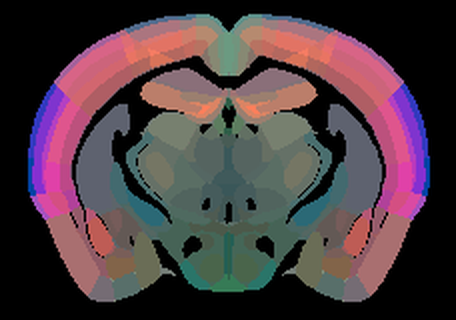
\includegraphics[width=.9\linewidth]{../results/pca_ano_coronal_50_res_slice_1.png}
		\caption{PCA coronal}
		\label{fig:PCA_cor}
	\end{subfigure}
	\begin{subfigure}{.176\textwidth}
		\centering
		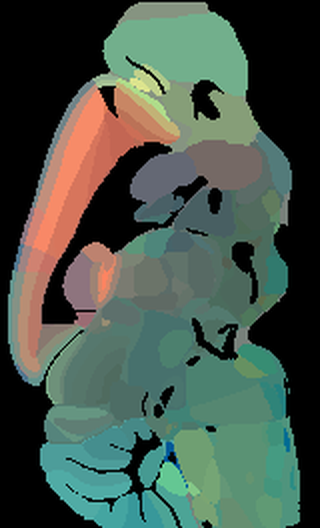
\includegraphics[width=.9\linewidth, angle=270]{../results/pca_ano_sagittal_50_res_slice_1.png}
		\caption{PCA sagittal}
		\label{fig:PCA_sag}
	\end{subfigure}\hspace{1.3cm}
	\begin{subfigure}{.25\textwidth}
		\centering
		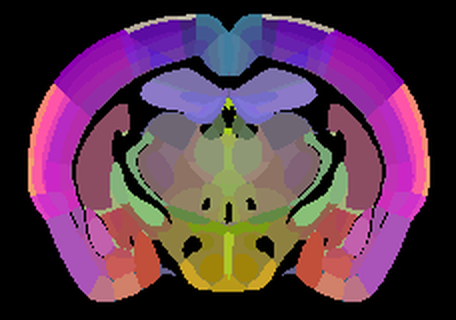
\includegraphics[width=.9\linewidth]{../results/tsne_ano_coronal_50_res_slice_1.png}
		\caption{T-SNE coronal}
		\label{fig:TSNE_cor}
	\end{subfigure}
	\begin{subfigure}{.176\textwidth}
		\centering
		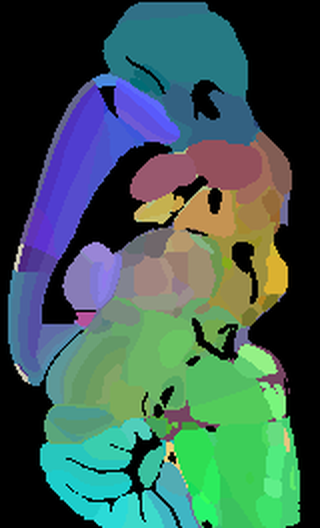
\includegraphics[width=.9\linewidth, angle=270]{../results/tsne_ano_sagittal_50_res_slice_1.png}
		\caption{T-SNE sagittal}
		\label{fig:TSNE_sag}
	\end{subfigure}\\

	\begin{subfigure}{.25\textwidth}
		\centering
		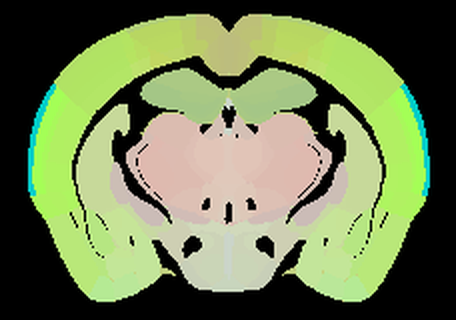
\includegraphics[width=.9\linewidth]{../results/umap_ano_coronal_50_res_slice_1.png}
		\caption{UMAP coronal}
		\label{fig:UMAP_cor}
	\end{subfigure}
	\begin{subfigure}{.176\textwidth}
		\centering
		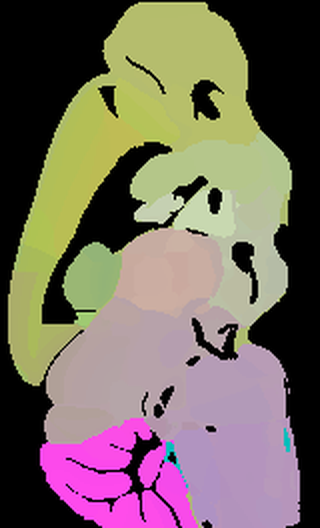
\includegraphics[width=.9\linewidth, angle=270]{../results/umap_ano_sagittal_50_res_slice_1.png}
		\caption{UMAP sagittal}
		\label{fig:UMAP_sag}
	\end{subfigure}\hspace{1.3cm}
	\begin{subfigure}{.25\textwidth}
		\centering
		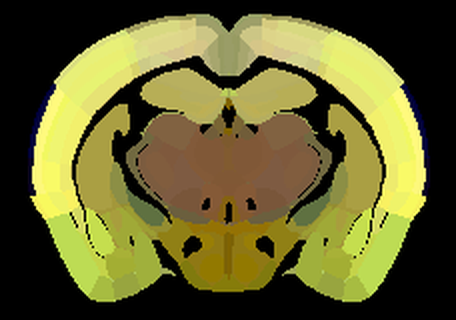
\includegraphics[width=.9\linewidth]{../results/para_umap_ano_coronal_50_res_slice_1.png}
		\caption{PaUMAP coronal}
		\label{fig:ParaUMAP_cor}
	\end{subfigure}
	\begin{subfigure}{.176\textwidth}
		\centering
		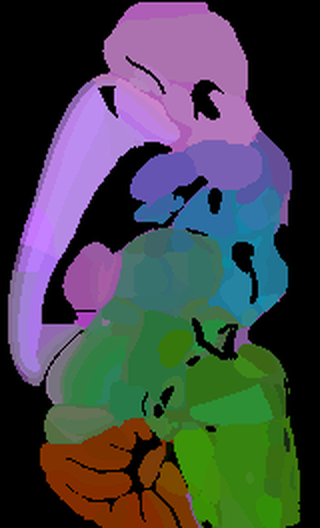
\includegraphics[width=.9\linewidth, angle=270]{../results/para_umap_ano_sagittal_50_res_slice_1.png}
		\caption{PaUMAP sag.}
		\label{fig:ParaUMAP_sag}
	\end{subfigure}\\

	\begin{subfigure}{.25\textwidth}
		\centering
		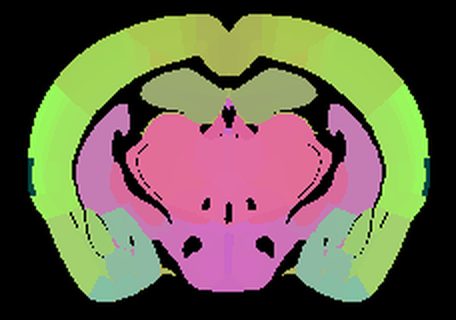
\includegraphics[width=.9\linewidth]{../results/para_umap_GCN_ano_coronal_50_res_slice_1.png}
		\caption{PaUMAP GCN}
		\label{fig:ParaUMAP_GCN_cor}
	\end{subfigure}
	\begin{subfigure}{.176\textwidth}
		\centering
		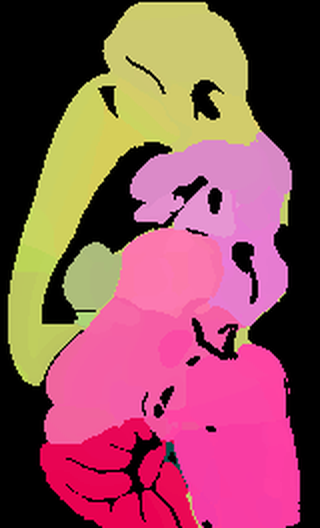
\includegraphics[width=.9\linewidth, angle=270]{../results/para_umap_GCN_ano_sagittal_50_res_slice_1.png}
		\caption{PaUMAP GCN}
		\label{fig:ParaUMAP_GCN_sag}
	\end{subfigure}\hspace{1.3cm}
	\begin{subfigure}{.25\textwidth}
		\centering
		
\includegraphics[width=.9\linewidth]{../results/para_umap_GAT_ano_coronal_50_res_slice_1.png}
		\caption{PaUMAP GAT}
		\label{fig:ParaUMAP_GAT_cor}
	\end{subfigure}
	\begin{subfigure}{.176\textwidth}
		\centering
		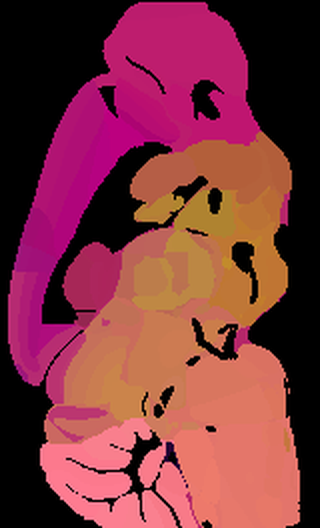
\includegraphics[width=.9\linewidth, angle=270]{../results/para_umap_GAT_ano_sagittal_50_res_slice_1.png}
		\caption{PaUMAP GAT}
		\label{fig:ParaUMAP_GAT_sag}
	\end{subfigure}\\

	\begin{subfigure}{.25\textwidth}
		\centering
		
\includegraphics[width=.9\linewidth]{../results/para_umap_GEN_ano_coronal_50_res_slice_1.png}
		\caption{PaUMAP GEN}
		\label{fig:ParaUMAP_GEN_cor}
	\end{subfigure}
	\begin{subfigure}{.176\textwidth}
		\centering
		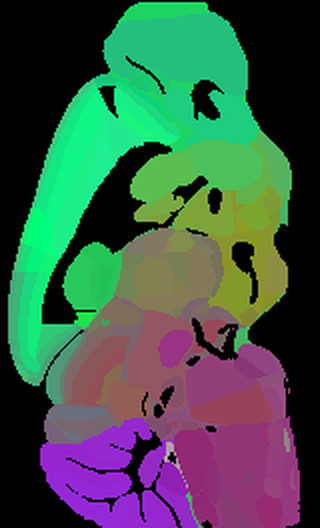
\includegraphics[width=.9\linewidth, angle=270]{../results/para_umap_GEN_ano_sagittal_50_res_slice_1.png}
		\caption{PaUMAP GEN}
		\label{fig:ParaUMAP_GEN_sag}
	\end{subfigure}\hspace{1.3cm}
	\begin{subfigure}{.25\textwidth}
		\centering
		
\includegraphics[width=.9\linewidth]{../results/para_umap_KerGNN_ano_coronal_50_res_slice_1.png}
		\caption{PaUMAP KerGNN}
		\label{fig:ParaUMAP_KerGNN_cor}
	\end{subfigure}
	\begin{subfigure}{.176\textwidth}
		\centering
		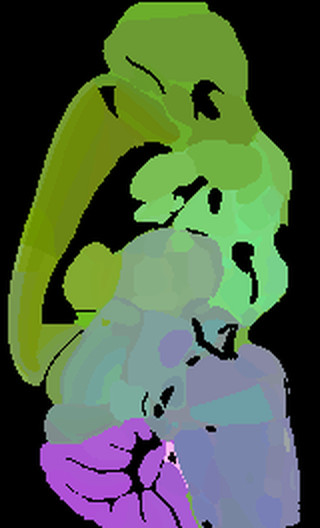
\includegraphics[width=.9\linewidth, angle=270]{../results/para_umap_KerGNN_ano_sagittal_50_res_slice_1.png}
		\caption{PaU KerGNN}
		\label{fig:ParaUMAP_KerGNN_sag}
	\end{subfigure}\\

	\caption[Resulting visualizations for all dimensionality reduction images]{(a) - (d): Resulting images for the baseline methods PCA and t-SNE; (e) - (h): Embedding visualization for neural network based dimensionality reduction methods UMAP and Parametric UMAP; (i) - (p): Parametric UMAP (PaUMAP, PaU) images exploiting graph convolutional neural networks in its encoding model formulation, demonstrating the oversmooting issue for GCNConv and GATConv, and fine grained results for GENConv and KerGNN}
	\label{fig:dim_red_vis}
\end{figure}


\begin{figure}
	\centering
	
	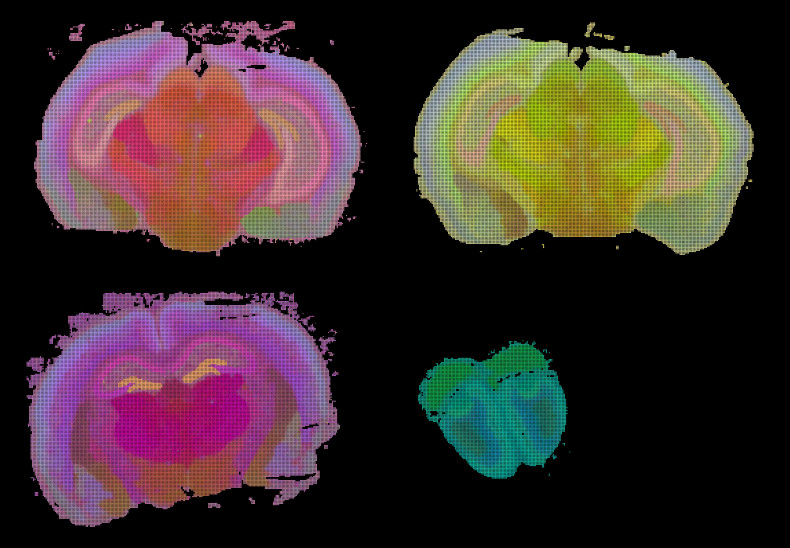
\includegraphics[width=0.5\textwidth]{figures/graphiss_anlaysis.jpg}
	
	\caption[Voxel-level dimensionality reduction baseline results]{Voxel-level dimensionality reduction results from \citet{Partel2020} utilizing UMAP serving as baseline}
	\label{fig:baseline_vis}
\end{figure}



Unfortunately, we could not find a suitable implementation of UMAP allowing for custom, deeper encoding models (though theoretically possible), but we were successful looking for suitable implementations for Parametric UMAP. Links and further links are given in the Github repository. \\

Thus, the following images and results are given with respect to deeper and thus more expressive neural network-based models than for UMAP. Moreover, we may re-use the UMAP loss, used as the optimization objective for UMAP and Parametric UMAP. It describes the proximity and boundness of simplices in the domain space, and how well they are preserved in lower dimensions.
For the non-graph convolutional baseline encoder for Parametric UMAP we run a manual grid search for the best set of hyperparameters. Moreover, we instantiated control neural network, consisting of the same layers as GENConv, but removed the message passing step. These two cases coincided, thus leading to the graph-less baseline method and its data shown in the right part of Table \ref{tab:dim_red_GCN}.\\
As base graph, we utilize the protein-protein interaction graph with associated gene expression value for each gene-protein pair as node feature. Thus every node only has a singular value as description. As encoding model for the combination with Parametric UMAP we applied the model shown in Figure \ref{fig:dim_red_mdel}. It consists of three stacked ResGraphConv Blocks allowing for deeper neural networks overcoming the oversmoothing of node features in GCNConv and GATConv, especially in highly connected graphs like our STRING-based PPI network.
However, this circumvention does not work for GCNConv and GATConv as seen in the respective results. The performance drops crucially in comparison to the non-GCN Parametric UMAP model with a considerable jump in both \textsc{EmbSim} and \textsc{EmbVar}. The latter indicates overly similar embeddings, which may be caused by the respective kernel filters and message passing scheme. This also applies for GATConv, which applies the same message passing approach as GCNConv. Both may be seen in their respective visualizations in Figure \ref{fig:ParaUMAP_GCN_cor} to \ref{fig:ParaUMAP_GAT_sag}.
A large increase in \textsc{EmbSim} and \textsc{EmbVar} may be see in juxtaposition to GENConv and KerGNN. Both methods try to overcome the oversmoothing issues with novel learnable weighting methods and a learnable softmax preserving strong signals for GENConv, and shadow graph construction for KerGNNs, cutting edges from the dense PPI network. An increase in both measures indicates much better embeddings, which may not be reproduced with non-GCN methods. This signifies both increased similarity and good spread across the representation space. The improvement of embeddings may also be observed in the gap in UMAP-loss, also indicating improved embeddings. The visualizations in Figure \ref{fig:ParaUMAP_GEN_cor} to \ref{fig:ParaUMAP_KerGNN_sag} show a noticeable difference in color space to GCNConv and GATConv, but are hard to describe and highly subject due to the differing color schemes.

Yet, we see a distinction in performance from GENConv to KerGNN in terms of UMAP-loss, which we are not able to explain but must be caused in the different formulations. We assume that some singular genes are highly predictive for the structures orientation, as indicated by the gene set experiments in \citet{Partel2020}. Thus, GENConv might be able to underline, propagate and preserve these features better. The authors show, that a small subset of about 20 genes is able to properly represent each structure over UMAP. We show, that this is only partly true and overly simplifies the underlying issue in Figure \ref{tab:dim_red_results}. We conclude that GCNs may be able to naturally select and derive importance measures for these decisive genes and their corresponding interactions, which non-GCN deep neural networks and traditional approaches, i.e. PCA and t-SNE, are incapable of.

\begin{figure}
	\centering
	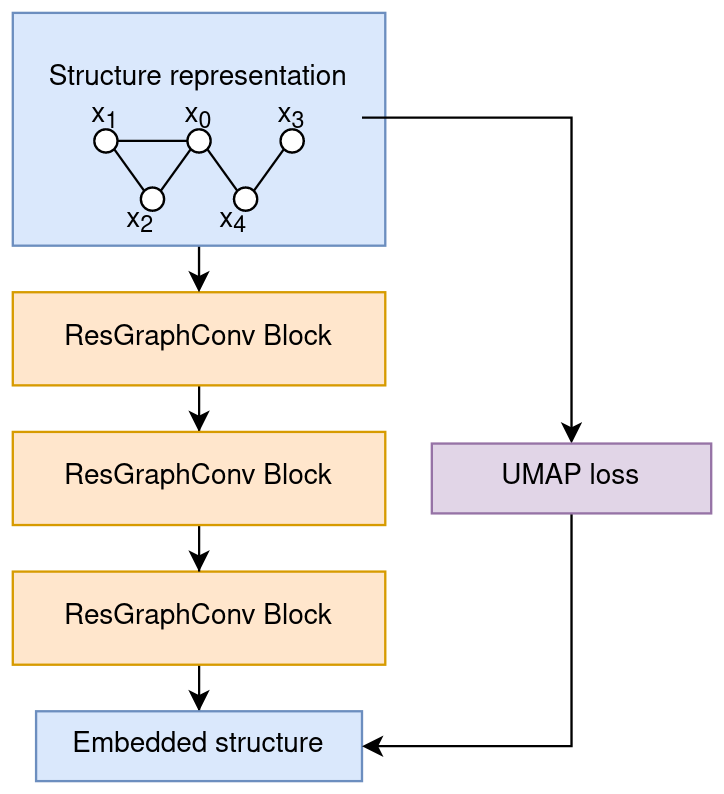
\includegraphics[width=0.4\textwidth]{figures/Dim_red_model_GCN.png}
	\caption{Encoding model's architecture, that was combined with Parametric UMAP for the task dimensionality reduction}
	\label{fig:dim_red_mdel}
\end{figure}



\subsection{On the linkage of connectivities and gene expression patterns}
\label{sec:results_connpred}
In this section we will describe the experiments and their outcomes for the connectivity prediction task. Here, we use normalized gene expression values as representations for each structure and predict the interactions between them. Further, the task is based on a two-entity prediction, whereas these entities are represented in the same representation space. 
This formulation causes a variety of challenges. Let us assume a na\"ive neural network (nNN) $f_{nNN}:\mathbb{R}^n\times \mathbb{R}^n\rightarrow [0,1]$ with parameterization $\Phi$ where inputs are bluntly concatenated and put through a series of linear neural layers, before being reduced to a dimensionality of $1$ by the output function. Moreover, let $s_1, s_2\in S$ be the gene expression-based representations of two structures in the mouse brain with $S$ the set of structure embeddings.
First, neural network models impose and assume an order among the inputs, indicated by the Cartesian product characterizing $f_{nNN}$'s domain. This causes $f_{nNN}(s_1, s_2)\neq f_{nNN}(s_2, s_1)$ for every distinct pair $s_1,s_2\in S$ with $s_1\neq s_2$. This may be solved by either a special regularization term in the model's loss function or my a special model structure. 
Second, we wish our model to be descriptive and explainable in terms of interpretability of results. Naturally, neural networks and their intermediate representation spaces are seldom understandable for humans. This is frequently done by a mapping into color space and the corresponding visualization. However, even if we assume the second to last layer of $f_{nNN}$ to be of dimensionality $k=3$, i.e. a bijective mapping to RGB color space exists, the meaning stays unsolved, as a convoluted, possibly non-trivial transformation of this space follows in form the neural output layer.\\

We aim to solve this issue by proposing a Siamese neural network\cite{bromley1993signature} (see \citet{chicco2021siamese} for an overview) for this purpose. Siamese neural networks (SNNs) embed the two considered entities from the same representation domain into the same embedding space. Here, the SNN optimizer tries to maximize the similarity of the two embeddings if linked and minimize the kinship for non-linked ones. This solves the two issues mentioned above. On one hand, as both entities are put through the same embedding model and the similarity function is commutative, SNNs are invariant to the order of their arguments. On the other hand, we may set the dimensionality of the embedding space to $k=3$ which is straightforward to visualize. Second, similar embeddings are embedded similarly imposing a natural structure among the embeddings. 
For the respective encoding model, we use a stacked architecture of ResGraphConv blocks (see Section \ref{sec:GENConv} for more information) to incorporate the chosen graph convolutional neural layers equivalently as in Section \ref{sec:results_dim_GCN}. Again, we use the ``flat'', non-GCN model as a baseline approach for our method. Again, we use the same architecture but remove the corresponding message passing step. Eventually, we use Cosine similarity as similarity metric.
The full model is shown in Figure \ref{fig:conn_pred_model}. Note that this model is the siamese formulation of the model in Figure \ref{fig:dim_red_mdel} and follows the same architecture, but mirrored.\\

While the input dimensionality is fixed among for all entities, the sembedding space dimensionality remains a crucial hyperparameter and thus a central research question. Naturally, the \textit{real} embedding space does not have to follow our desire for visualizations and better understanding. We thus analyze the impact of the output dimensionality on the predictive performance and descriptive capabilities of the SNN. We hence choose $k\in \{3,20\}$ as representatives for a better understanding.\\

The results of our experiments are shown in Table \ref{tab:results_connpred_20} and \ref{tab:results_connpred_3}. Here, results are computed over a 5-fold cross validation on the full set of pairs of structures. Both experiment sets follow the same random seed for their splits, and hence share the collection of structures in training and validation phase for different choices of $k$. However, we have different sets of structures for structural, and functional and effective connectivity (see Section \ref{sec:datasets} for more information and numbers). 
From the results, we may conclude that all predictors were able to grasp the underlying signal. The predictive performance was higher than $0.60$ in terms of AUROC score with exception to only one data point. Moreover, we see a surprisingly high AUC  around $0.75$ for dimensionality $k=20$, but a noticeable drop in score towards lower dimensionality. This may indicate that the underlying dimensionality of connectivity is larger than three, and will be discussed further in Section \ref{sec:discussion}.

Crucially, the dimensionality reduction experiments in Section \ref{sec:results_dim_GCN} behave likewise to the observed ones here. Again, GCNConv and GATConv were not able to provide any additional performance gain, which may be again due to lacking ability to highlight and identify important substructures within the PPI graph. Furthermore, GCNConv's and GATConv message passing algorithm lead non-convergence of the model in a number of cases, inducing very low scores in both functional and effective connectivity, primarily in the lower-dimensional $k=3$ case. 
Most importantly, we observe a consistent performance increase across all types of connectivity using GENConv and KerGNN. This is clearly visible for both displayed dimensionalities $k\in \{3,20\}$. GENConv and KerGNN seem to observe underlying patterns that are descriptive of the brains connectivity, not only for axonal and functional connectivity, but also for effective connectivity, on which only little literature may be found. \\

We hence conclude that GCNs over protein-protein interaction graphs help to identify crucial patterns within the gene expression values for all sub-types of connectivity. 

\begin{table}
	\centering
	\renewcommand{\arraystretch}{1.2}
	\begin{subfigure}{1.\textwidth}
		\centering
		\begin{tabular}{|l|l|l|l|l|l|}
			\hline
			&\multicolumn{5}{c|}{GCN layer type}\\
			Connectivity type&None&\textsc{GCN}&\textsc{GAT}&\textsc{GEN}&\textsc{KerGNN}\\
			\hline
			Struc conn&0.80&0.73&0.76&0.82&0.83\\
			Funn conn&0.76&0.72&0.73&0.79&0.81\\
			Eff conn&0.77&0.75&0.75&0.79&0.78\\		
			\hline
		\end{tabular}
	
		\caption{AUROC scores for embedding dim $k=20$}
		\label{tab:results_connpred_20}
	\end{subfigure}\\

	\begin{subfigure}{1.0\textwidth}
		\vspace{0.5cm}
		\centering
		\begin{tabular}{|l|l|l|l|l|l|}
			\hline
			&\multicolumn{5}{c|}{GCN layer type}\\
			Connectivity type&None&\textsc{GCN}&\textsc{GAT}&\textsc{GEN}&\textsc{KerGNN}\\
			\hline
			Struc conn&0.70&0.68&0.67&0.72&0.73\\
			Funn conn&0.64&0.54&0.61&0.66&0.68\\
			Eff conn&0.69&0.60&0.60&0.69&0.71\\		
			\hline
		\end{tabular}
		
		\caption{AUROC scores for embedding dim $k=3$}
		\label{tab:results_connpred_3}
	\end{subfigure}	
	\caption[AUROC scores for our experiments on the prediction of connectivities from gene expression values for embedding dimensions $k\in \{3,20\}$]{AUROC scores for our experiments on the prediction of connectivities from gene expression values for embedding dimensions $k\in \{3,20\}$. We compare GCN-based and non-GCN-based models for this purpose.}
	\label{tab:conn_pred_GCN}
\end{table}

\begin{figure}
	\centering
	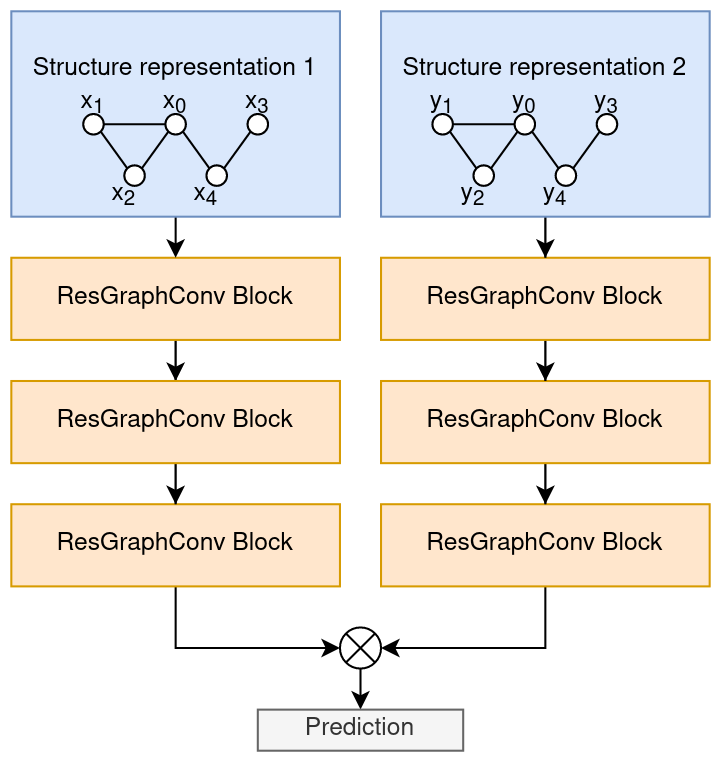
\includegraphics[width=0.5\textwidth]{figures/ConnPred_model.png}
	
	\caption[Siamese neural network architecture used for the prediction of connectivities based on gene expression patterns]{Siamese neural network architecture used for the prediction of connectivities based on gene expression patterns. Inputs are node labels $x_0, \dots, x_N$ and $ y_0, \dots, y_N$, i.e. gene expression values, annotated to the same PPI graph. $\otimes:\mathbb{R}^k\times\mathbb{R}^k\rightarrow[0,1]$ denotes a symmetric similarity function, i.e. cosine similarity. Crucial hyperparameter is the embedding dimensionality $k$. }
	\label{fig:conn_pred_model}
\end{figure}

%\subsection*{Brief Overview of Material}
%\subsection*{Findings (Results) of the Method of Study and Any Unplanned or Unexpected Situations that Occurred}
%\subsection*{Brief Descriptive Analysis
%Reliability and Validity of the Analysis}
%\subsection*{Explanation of the Hypothesis and Precise and Exact Data (Do Not Give Your Opinion)}


\newpage
\section{Discussion}
\label{sec:discussion}

Within this discussion we will elaborate on the answers and experiments of the results chapter. This chapter is divided into three sub-sections following the results of the respective trial groups. 

\subsection{Evaluating different feature types for gene expression prediction}
\label{sec:disc_genexp}
First, we evaluate the conclusions and materials of the gene expression prediction task. Here, we predicted gene expression values across different brain compartments based on varying feature types and tried to incorporate spatial models and background knowledge in our prediction task. \\

Based on the strong results in \citet{schulte2021integration} and \citet{wang2021mogonet}, predicting gene expression values in human tissue from molecular features, we expected these experiments to work out much better. Especially the weakness of GENConv, that was successfully applied to a variety of problems, e.g. in the other two tasks, was particularly surprising. 
We expect molecular features, i.e. ``bottom-up representations'' to not be exploitable over protein-protein interaction graphs as molecular descriptors are very protein and gene specific. Thus, neighbors in the interaction network may not be able to benefit from information about their respective adjacents in pathways. The phenotypical, i.e. ``top-down'', representations describe properties of sets of proteins with specific functions. As this function may likely be shared among proteins within pathways, i.e. a neighborhood within the PPI graph, we do expect GCNs to benefit. Similar results were indicated for the related task drug-target interaction prediction in \citet{hinnerichs2021dti}, requiring a strong and functional representation for proteins, too. \\

Yet, we see that these assumptions and hypotheses do not hold within the mouse brain over none of the tested brain divisions. This may be due to two rationales. First, in comparison to the works mentioned, we try to infer the transcriptome in neural tissues. As these compartments are very different from other tissues, e.g. are situated within a separate nutritional network, they also follow different sets of phenotypes. The features mentioned above are mainly fit against ground truth functions such as \textit{Tachykardia} or pathological symptoms such as \textit{coughing}, that are only valuable for other organs. While there might even be a correlation between these two phenotypes  (cough correlates with viral infections, causing fever and hence high-levels of circulatory activities) their correlation with brain division is yet to be found. Second, gene expression might be too protein specific for graph convolution to grasp. GCNs are only capable of learning a fixed, small set of kernels which are applied to all proteins at once for deriving node-level predictions. We assume that these kernels are too diverse to properly pick up for smaller networks. This may be either overcome using large sets of independent kernels such as in \citet{schulte2021integration}, or by a non-GCN approaches, modeling all edges in the PPI graph by separate neural networks. The latter may be very insightful to further understand specific protein-protein interactions and their impact on the gene expression. \\

Due to the specificity of the tissue, task and approach, we were not able to find a suitable baseline method in the literature, and thus are the first to test this very hypothesis. However, the hypothesis was to find such correlation, and we eventually have to reject this assumption.\\

Eventually, we were not able to derive a natural formulation to incorporate both spatial knowledge and gene-specific features into a single model. We moreover stopped all experiments after the extensive experiments for this very task failed to show any improvement over the non-GCN baseline. Possible encodings for this task may include structure specific representations, e.g. a random walk-based method on the structure ontology describing the spatial orientation within the mouse brain, or a graph learning approach over the structure ontology. However, the latter may be infeasible for regular message passing schemes to grasp and should rely on a more sophisticated and expressive model formulations.


%\subsection*{Brief Overview of Material}
%\subsection*{Full Discussion of Findings (Results) and Implications}
%\subsection*{Full Discussion of Research Analysis of Findings}
%\subsection*{Full Discussion of Hypothesis and of Findings}
%\subsection*{Post Analysis and Implications of Hypothesis and of Findings}

\subsection{Gene expression patterns and their relation to GCNs}
\label{sec:disc_dimred}
The experiments on dimensionality reduction were crucially more successful. We first showed the validity of \textsc{EmbSim} and \textsc{EmbVar} and show through various experiments that both metrics are necessary to properly evaluate and show improvement over baseline methods. This step is central and vital for the entire following validity and genuineness of our results. However, we see clear issues in both formulations. We originally tried to formulate a measure that is able to overcome both the random and the ``narrow gaussian'' signals. Yet, we were not able to formulate a measure such that the qualified assessment directly correlates with our understanding of \textit{reasonable} and \textit{natural} embeddings and their properties. With our formulation of \textsc{EmbSim} and \textsc{EmbVar}, allowing for robustness against choice of structures, further assessment of the sub-compartments smoothness may be made. 
We thus conduct a follow-up study to further analyze the performance of all dimensionality reduction approaches on sets of sub-structures. Comparing kinship of raw and encoded structures across proximate entities based on k-nearest neighbor clustering (KNN) does not show remarkable deviations, once again proving the correctness of our embeddings. 
Additionally, we see a indirect correlation of UMAP loss and \textsc{EmbSim}. The UMAP loss describing the proximity of entities in embedding space in correlation with neighborhood in the domain representation space, decreases whenever \textsc{EmbSim} and vice versa. This indicates the high similarity of gene expression values within compartments on one hand, and thus the legitimacy of our biological hypothesis underlying \textsc{EmbSim} and \textsc{EmbVar} on the other hand. \\

Second, we were able to show the importance of the normalization technique for the biological assumption, data diversity and embedding complexity. Hence, we observe an performance gain for PCA in comparison to the other proposed normalization schemes. We thus conclude that a column-wise, i.e. per-gene, normalization does indeed help highlighting\textit{effective genes} and penalizes \textit{ineffective genes}, and shows the existence of both.\\

Contrary to the gene expression prediction task, we were able show consistent performance increase across all considered metrics, i.e. \textsc{EmbSim}, \textsc{EmbVar} and UMAP loss, by applying GENConv and KerGNN as convolutional graph layers. The large sample size of $843$ structures may indicate the legitimacy of the results. Experimental setups and hyperparameter configurations suffer from high sensitivity and reduced robustness, and thus are in need for careful adjustments. For that very reason, even though we were able to consistently grasp the added signal within our experiments, information may not be automatically perceived by blind usage of graph convolutional approaches.

%Yet, we struggle to reason the particular experiment outcomes. While the issue of over-smoothing for GCNConv and GATConv are known and clearly visible from the results, the improved score for GENConv and KerGNN remains is non-trivial. 
In \citet{Partel2020} and \citet{bohland2010clustering}, the authors show the importance of a subset of genes for description of gene expression patterns. We hypothesize that the pathway information, encoded in the interaction network, may contain information not only about the gene importance, but also on inter-gene relation, possibly for down-stream processes. We expand this discussion in Section \ref{sec:disc_connpred}. An in-depth analysis of these gene interactions, e.g. by exploiting the explainability of GCNs over activation heatmaps, may be subject to future projects but will possibly provide novel insights to gene importance and influence. \\

Even though we showed a distinction under the proposed metrics, the visualizations of structure embeddings in Figure \ref{fig:baseline_vis} are of limited value for such comparisons. As all embeddings have own ways of distributing entities in the embedding, i.e. color, space, the varying color schemes conceal the underlying differences, thus leaving us with vague descriptions of RGB tendencies. Unfortunately, there is no trivial way to overcome this issue. However, these visualizations are great to show the spatial distribution and structural color trends over all methods.
 
Across all experiments we notice a continuous gene expression gradient in the sagittal cross-section, while the coronal cross-section shows clear distinctions in color space in-line with \citet{Partel2020} and \citet{sansom2009gradients}. This gradient is described by the an alteration of expressions especially in the \textit{Isocortex} and its sub-regions, i.e. \textit{Frontal pole}, \textit{Somatomotor areas} (layer 1 to 6b), \textit{Primary}  and \textit{Secondary motor areas} (layer 1 to 6b) and \textit{Somatosensory areas} and other sensing related areas. While these structures are fairly similar in transcriptomic values, we notice an increased amount protein-protein interactions in between \textit{shifting genes}, i.e. genes with changing expression value, across neighboring structures in e.g. \textit{Somatosensory areas}. Moreover, all \textit{shifting genes} are connected to at least one expressing gene in the PPI graph, which may cause the capability of GCNs for \textit{smoother} representations. \\

\begin{figure}
%	\centering
	\hspace{1.5cm}
	\begin{subfigure}{.4\textwidth}
		\centering
		
\includegraphics[width=.9\linewidth]{../results/para_umap_GEN_ano_coronal_50_res_clus_slice_1.png}
		\caption{PaUMAP GENConv cor.}
		\label{fig:disc_clustering_cor}
	\end{subfigure}
	\begin{subfigure}{.28\textwidth}
		\centering
		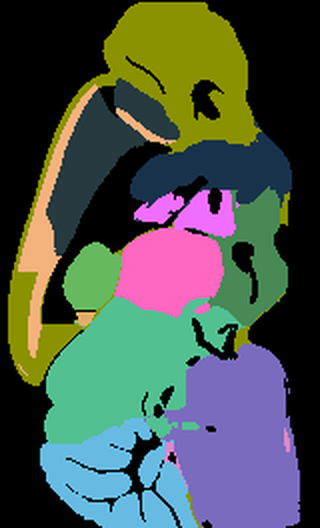
\includegraphics[width=.9\linewidth, angle=270]{../results/para_umap_GEN_ano_sagittal_50_res_clus_slice_1.png}
		\caption{PaUMAP GENConv sag.}
		\label{fig:disc_clustering_sag}
	\end{subfigure}\\
	
	\caption[Visualization of clustered gene expression patterns over GENConv-enhanced Parametric UMAP model outputs]{Visualization of clustered gene expression patterns over GENConv-enhanced Parametric UMAP model outputs. Clustering was done under usage of k-nearest neighbors with $k=16$, the number of top-level compartments defined by $CCFv3$}
	\label{fig:disc_clustering}
\end{figure}


We take the chance to apply crisp clustering in form of k-nearest neighbors (KNN) to the derived encodings, in order to construct distinguishable expression patterns. We fix $k=16$, with respect to the number of top-level sub-compartments described by the structure ontology (CCFv3). The results are depicted in Figure \ref{fig:disc_clustering}. This visualization shows direct correspondence with the parcelation of CCFv3. However, this analysis is strictly bound to the divisions defined in the Allen Mouse Brain atlas, and may not be feasible for discovery of novel subdivisions, like e.g. \citet{takata_flexible_2021} directly using the underlying voxels. Yet we were able to show the inter-structure similarity within neighborhood and thus may, without loss of generality, assume the smoothness of expression within compartments and the legitimacy for consideration of summaries of voxels, i.e. structures. The voxel-wise application of GCNs will remain an open research question, but will surely require enormous computational power as $\approx500^3$ voxels exist for $25 \mu m$ in contrast to the $834$ considered structures.\\



%
%
%\begin{itemize}
%	\item influence of normalization technique $\rightarrow$ Structure, gene, global
%	
%	\item no integration with UMAP possible due to missing implementation of UMAP in PyTorch
%	\item dimensionality of encoding embedding to be done
%	\item what do these novel embedding yield as insights?
%	\item different distance metrics
%	\item correlation of UMAP loss and our metrics shows both the validity of our method, but also the similarity of gene expression values within compartments (see Table \ref{tab:gen_red_baseline})
%	\item no real additional insight from GCN based visualizations
%	\item no clustering as it only makes sense in the coronal cross-section $\rightarrow$ sagittal section show clear gradient
%	\item fragile experiments
%\end{itemize}

\subsection{Connectivity prediction and brain dimensionality}
\label{sec:disc_connpred}
Third we will discuss the experiments and the underlying assumptions for the task of connectivity prediction.
Recurrently, we see that neural networks are indeed able to capture the latent and fundamental signal determining connectivity. Furthermore, we are able to re-apply the same model architecture, that showed major performance increase in the dimensionality reduction task, within a siamese network formulation for similarity-based connectivity prediction. Again, we see a noticeable improvement over the non-GCN baseline method.\\

The sketched performance improvement is naturally surprising due to the difference in time scales of features in comparison to the particular connectivity types. As detailed in Section \ref{sec:datasets}, axonal, functional and effective links are ranging within an entirely differing temporal proportion than transcriptomic data. Axonal wiring may be dynamic over hours to months, while effective and functional relations may be re-arranged within minutes, describing e.g. the cognitive process of learning and adaption \cite{van2010exploring, friston1994functional, friston1993functional, sporns2016networks}. On the other hand gene expression may alter rapidly, too, but remains generally stationary and constant due to its high correlation with spatiality \cite{Partel2020, bohland2010clustering} and embryogenesis \cite{zapala2005adult, dillman2013mrna}. This correlation may be result of ion channel priming in ion channels determining synaptic functions such as transmission of neurotransmitters. This effect was specified in \citet{richiardi2015correlated} to over-expression of genes associated with sodium channels such as SCN4B or receptors such as GABRA5, but also potassium channels. Moreover, the expressed genes were primarily linked to Gene Ontology functions and processes \cite{GOoriginal2000, GOrecent2020} such as receptor and channel activity. The high number of links within the protein-protein interaction network may cause the improved performance by our used graph convolutional methods. We conclude that genetic expression may be a prior for neural activation patterns in inter-compartment connectivity, and may be characterized by patterns in the interaction network.\\

Here, we will describe the set of chosen hyperparameters, and more specifically the chosen dimensionality $k$. As seen in the results this parameter crucially correlates with the models performance in the prediction task, as it describes the model's ability to remember and describe entities in lower dimensions. With an artificial information bottleneck with $k=3$, we are able to map the structures in to color space for a visualization of the respective results. 
However, with $k=3$ chosen, the predictive capability drops, thus inducing that this may not be the \textit{true dimensionality} of the respective connectivity realm. As functional and effective connectivity have direct links to cognition and its pathology, constructing a capturing manifold may benefit better understanding of neural activity and thinking. Neural manifolds were able to model e.g. spatial orientation of mice in test scenarios \cite{nieh2021geometry, stringer2019high}. Axonal connectivity and its disturbances is further linked to variety of diseases as described in the related work Section \ref{sec:relatedwork}. 
Consequently, we compute the AUROC performance in the interval $k\in \{3,4,\dots,20\}$ to determine the underlying manifold. Observed scores are depicted in Figure \ref{fig:disc_dim_trend}, where we notice an almost linear correlation of dimensionality $k$ and AUROC score across all three considered connectivity types. As no clear edge is given within the three experiment sets, we may not answer this question precisely. However, we may see a clear upwards trend for which a infimum must exist. Thus, successively increasing the dimensionality will eventually reach this very infimum for some $k_{\inf, \text{conn}}$, which may describe the targeted connectivity for each connectivity type, respectively. Due to limited computing time and power, we leave this as a future research question. Nonetheless, this threshold was not reached in the considered interval, which we regard as \textit{sufficiently small} with respect to a starting point for further manifold-based analysis. This \textit{descriptive dimensionality} may be both dependent on model architecture and entity representations, and their corresponding expressivity. Additionally, for a given descriptive dimensionality $k_{\inf, \text{conn}}$ a follow-up study on the combined dimensionality may yield more insights into the underlying neural geometry and cognitive manifolds, but stays outside of the scope of this work. \\

\begin{figure}
	\centering
	\includegraphics[width=0.9\textwidth]{plotted_figures/dimensionality_trend.png}
	
	\caption{AUROC scores for different embedding dimensionalities $k$ for the three different connectivity types}
	\label{fig:disc_dim_trend}
\end{figure}

Despite the great results and insights, our work is exposed to two limitations. First, is the legitimacy of connectivity data, and more specifically effective connectivity. Reported in Section \ref{sec:datasets}, we derive the causal relationships by usage of instrumental variables \cite{angrist2009mostly, pearl2009causality, baiocchi2014instrumental}. The endowment of priors on unknown parameters is crucial for the identification of eventual causal dependencies. As these priors remain unknown for the given data, various assumptions have to be made, and may often correlate with functional connectivity due to the computation. Fortunately, effective and functional links express different patterns for our data as depicted in Figure \ref{fig:conn_vis}. For an expanded discussion on the legitimacy of instrumental variables for fMRI data see \citet{valdes2011effective}.
The second limitation of this work lies within the coarseness of the considered structures and divisions. While we analyzed $843$ sub-structures and their respective gene expression values in the tasks of gene expression prediction and dimensionality reduction, only $49$ unique and distinct structures were utilized in \citet{AIDAmri2019} for functional and effective connectivity, and $147$ structures for axonal projection data. This not only impairs the statistical soundness of our experiments, but also constraints the number of follow-up analyses. We are not able to analyze of predict on e.g. the connectivity within the \textit{Cerebellum}, showing the generalizability of the method and model, as it consists of only two, connected sub-structures. Specifically, the Cerebellum shows distinct gene expression patterns in Figure \ref{fig:dim_red_vis} and consequently an analysis of its position in the connectivity prediction embedding space would benefit the outcome and interpretation of this work. Similar constraints hold for the \textit{Isocortex} and the \textit{Olfactory bulb}. Particularly the Olfactory bulb and its analysis would crucially benefit and advance the work on olfactory signaling within the Neural Data Science (NeurDS) group at the Max Planck Institute for Human Cognitive and Brain Sciences (MPI: CBS).
On the other hand, we may not be able to conduct these experiments on the voxel level. Functional magnetic resonance imaging (fMRI) is prone to noise and hence is often considered with respect to regions-of-interest (ROIs). Within the AIDAmri project \cite{AIDAmri2019} and its dataset, these ROIs were set to the respective structures defined by the Common Coordinate Framework (CCFv3). Thus we rely on open-source mouse brain fMRI data, which is rarely available. Even the processing of the AIDAmri data with the associated AIDAconnect  pipeline (proposed by the same group) took several weeks to finish due to expandable suitability and matching of both. The structure-wise computation not only made experiments finish within reasonable, yet significantly large time, but also allowed for reinforcement of the underlying signal.

The application of GCN methods on individual voxels may be computationally infeasible, but simpler, less expressive graph convolutional models, e.g. with less layers, may allow for such calculations.\\

In this work, we only studied the brain patterns and connectivities within health and normal mice. The model formulation allows for direct investigation on perturbations across all three connectivity types and the influence of the gene expression prior. Genetic markers were associated with schizophrenia and affective disorders \cite{blackwood2001schizophrenia} and obsessive-compulsive disorders \cite{hall2003sequence}. Moreover, these are linked to perturbations in functional and effective connectivity \cite{friston2002dysfunctional, friston2011functional}. An extensive analysis of this prior and the predictive capabilities of the proposed model are outside the scope of this work, yet are highly influential for better understanding of underlying biological- and neurological processes and priors.\\

In our experiments moving from spatial gene expression patterns towards their linkage to connectivities, we considered other approaches for incorporation of inter-structure networks. The most promising idea was to extend the idea of the UMAP loss and its graph with an external graph, modeling the associations. The UMAP formulation then tries to not only embed proximity within domain representation space, but also adjacency in the connectivity network. This would allow for similar embeddings like the SNN, but requires a custom formulation and weighting of the two networks, which are mutually independent. We run several experiments under these assumptions and various weights, but the network collapsed to either of the two formulations. Primarily, the connectivity lacks a suitable distance measure which is given for the pure UMAP graph based on its distance measurement. Thus, constant and arbitrary distances need to be defined, also describing the weighting of the respective networks. Due to the lacking natural intuition for such weighting and the poor results for all tested weights, we moved over to the Siamese neural network, which eventually returned great results.\\

One of the most fundamental questions of our work is the puzzle of generalization. We showed, that this particular network formulation does hold for model organism such as \textit{Mus musculus}, i.e. smaller mammals such as rodents. However, it still remains questionable whether similar experiments in more complex mammals such as apes, monkeys such as Macaques \cite{ValkShapingBrainStructure2020} and eventually humans still hold true. The increased complexity of neural activity and larger dimensionality of cognition may indicate pitfalls for a re-application of this very approach, but has yet to be tested in actual experiments and thus future work.\\

\subsection{Novelty and Contributions}
Within this work we made several contributions and discovered several findings. We provide the first method to apply graph convolutional neural networks for prediction of and based on gene expression data within the mouse brain. Further, introduced two evaluation metrics that prove the validity of improvements of GCN-enhanced methods over the baseline algorithms for dimensionality reduction and spatial pattern recognition. We do an extensive analysis of normalization schemes and the biological implications of these results. Further, we show that the same model consistently improves other down-stream tasks, such as connectivity prediction over three different connectivity types, and link these findings to related results from the literature.\\

We further contribute an open-source implementation of KerGNN \cite{feng2022kergnns} to the PyTorch Geomtric library \cite{PytorchGeometric}. Additionally, we made several contributions to solve the issues of the AIDAconnect pipeline (\href{https://github.com/aswendtlab/AIDAconnect}{github.com/aswendtlab/AIDAconnect}) and provide all precomputed features for future projects. Third, I built multiple open-source pipelines on open-source data for gene expression, structural connectivity, fMRI, functional connectivity and effective connectivity data aggregation and preprocessing, and their respective registration to the Allen Institute Common Coordinate Framework for the NeurDS group Max Planck Institute for Human Cognitive and Brain Sciences for future research projects.


%\begin{itemize}
%	\item we reduce to three dimensions, but there does not necessarily needs to be a 3D-representation
%	\item naturally, much better results with higher embedding dimension $\rightarrow$ poor visualization possibilities
%	\item only few structures considered
%	\item eff conn and fun conn seem somewhat correlated, thus similar predictive performance of all approaches $\rightarrow$ how feasible are instrumental variables for effective correlation modeling
%	\item parcelation is quite coarse, thus we cannot predict on separate structures $\rightarrow$ Results are to be taken with care
%	\item what is the dimensionality of conn pred?
%	\item biological meaning:
%	\begin{itemize}
%		\item different time-scale of observations
%		\item genetic expression may be a prior for neural activation patterns 
%	\end{itemize}
%	\item we considered including connectivity graphs into UMAP-loss, but no natural formulation for combination is possible. Here an artificial weighting of respective UMAP proximity graph and external connectivity graph is necessary. We conducted several experiments \dots. Collapses to either side, namely either overly weighting embedding proximity or connectivity matrix. We could not define a stable set of parameters for this to work.
%	\item approach is not limited to gene expression data, but may also be applied to other structure or regions-of-interest (ROI) focused representations, such as embeddings of e.g. neural activities 
%	\item May be applicable to analysis of the \textit{Disconnection Hypothesis} (see intro for more information)
%	\item how does this generalize to other model organisms or even humans?
%\end{itemize}

%Novelty:
%\begin{itemize}
%	\item GCNs over gene expression was never applied here
%\end{itemize}
%
%Contribution of this work:
%\begin{itemize}
%	\item Open source contribution, contributing a KerGNN implementation to PyTorch Geometric
%	\item Contribution to AIDAconnect project and enhanced their pipeline
%	\item Built plenty of pipelines on open-source data for the NeurDS group at CBS
%\end{itemize}



\newpage
\section{Conclusion}
\label{sec:conclusion}
In this work, we propose an extensive analysis on the influence of graph convolutional neural networks over protein-protein interaction graphs on gene expression prediction and further down-stream tasks. We thus first analyzed the influence of different feature types, i.e. molecular and phenotypic features, for their respective influence on forecasting the transcriptome. Yet, we were not able to see an evident increase in expressivity and predictive performance. 
Second, we integrate graph convolutional neural networks into Parametric UMAP and show its consistent increase over the non-GCN baseline. We therefore propose two metrics \textsc{EmbSim} and \textsc{EmbVar}, and show their corresponding legitimacy. The associated \textit{shifting genes}
within the gene expression gradient are (1) connected over the PPI network to expressed genes, which (2) are highly associated with ion channel activity.
Third, we re-use the same encoding model within a Siamese neural network to predict structural, functional and effective connectivity within the mouse brain. Anew, we see an increase in expressivity over the two special convolutional filter formulation, i.e. GENConv and KerGNN, which(1) extend the message passing scheme and (2) exploit the learning of hidden subgraphs. We show that the same \textit{shifting genes} from the second task are highly predictive for such interactions. 

We assume that the proposed encoding model may not only be able to evaluate \textit{gene importance}, which other works showed to be highly predictive for both dimensionality reduction and connectivity correlation, but also grasps the corresponding inter-gene relations. These inter-gene patterns are directly linked to neural activation patterns. While inter-structure relations were studied extensively, our work may spark future research in these inter-gene relations and patterns for better understanding of the mouse brain. \\

However, this work contains inherent limitations that may initiate future research work. Initially, we only consider the less complex and well studied rodent model organism of \textit{Mus musculus} and proved the importance of GCNs. Yet, a generalization of these results to more sophisticated organisms like macaques and even humans is still left open and non-trivial. Second, this analysis was only done on structure level, defined by the Allen Institute Common Coordinate Framework (CCF). CCF defines sub-divisions based on their morphology and we were able to show the inter-structure similarity across the brain, justifying the intra-structure similarity of expressions. Yet, in order to better understand the spatial brain compartments voxel-wise analysis remains mandatory. Additionally, an incorporation of developmental relations in the analysis in form of, e.g. neural and embryogenesis ontologies, integrating rich background knowledge may benefit such parcelations.
Third, we only verified the advances for two graph convolutional filters. However, as graph learning is currently among the most investigated research topics in machine learning, more and more complex graph kernels and methods are proposed. These kernels inherently follow different assumptions and thus may be able to show different properties and interpretations of inter-gene patterns facilitating further intuition. 
Fourth, we only studied the brain patterns and connectivities within sane mice. The model directly allows for analysis of perturbations, both in gene expression and connectivity. Further investigation of brain disease associated genetic markers over the proposed model may enhance the intuition on underlying biological processes and their pathology.

%Future work.
%\begin{itemize}
%	\item other GCN kernels associated with other interpretations
%	\item voxel level analysis
%	\item move to more complex organisms like macaques and humans
%	\item analysis of gene knockout and influence of connectivity
%\end{itemize}
%
%
%
%
%
%\subsection*{Summary of Academic Study}
%\subsection*{Reference to Literature Review}
%\subsection*{Implications of Academic Study}
%\subsection*{Limitations of the Theory or Method of Research}
%\subsection*{Recommendations or Suggestions of Future Academic Study}
%
%\begin{itemize}
%	\item gene expression patterns within mouse brain and both possible hypothesis and tasks, and models over this
%	\item gene knockout models and whether they can learn propagation of those?
%	\item connection of FC and gene expression patterns and how to prove such interaction/correlation?
%	\item possible gene knockout targets within mouse brain and possible structural influences
%\end{itemize}


\newpage

\bibliography{citations}

\newpage

\appendix



\end{document}